\documentclass[journal]{IEEEtran}
\usepackage[a5paper, margin=10mm]{geometry}
%\usepackage{lmodern} % Ensure lmodern is loaded for pdflatex
\usepackage{tfrupee} % Include tfrupee package


\setlength{\headheight}{1cm} % Set the height of the header box
\setlength{\headsep}{0mm}     % Set the distance between the header box and the top of the text


%\usepackage[a5paper, top=10mm, bottom=10mm, left=10mm, right=10mm]{geometry}

%
\usepackage{gvv-book}
\usepackage{gvv}
%\setlength{\intextsep}{10pt} % Space between text and floats

\makeindex

\begin{document}
\bibliographystyle{IEEEtran}
\onecolumn


\title{
	%\begin{flushleft}
	\begin{center}
	%MATRICES \\ In Geometry
	Discrete Mathematics
	\\
\rule{0.4\columnwidth}{0.4pt}
%\end{flushleft}
\end{center}
}
\author{
\vspace{11cm}
	%\begin{flushleft}
	\begin{center}
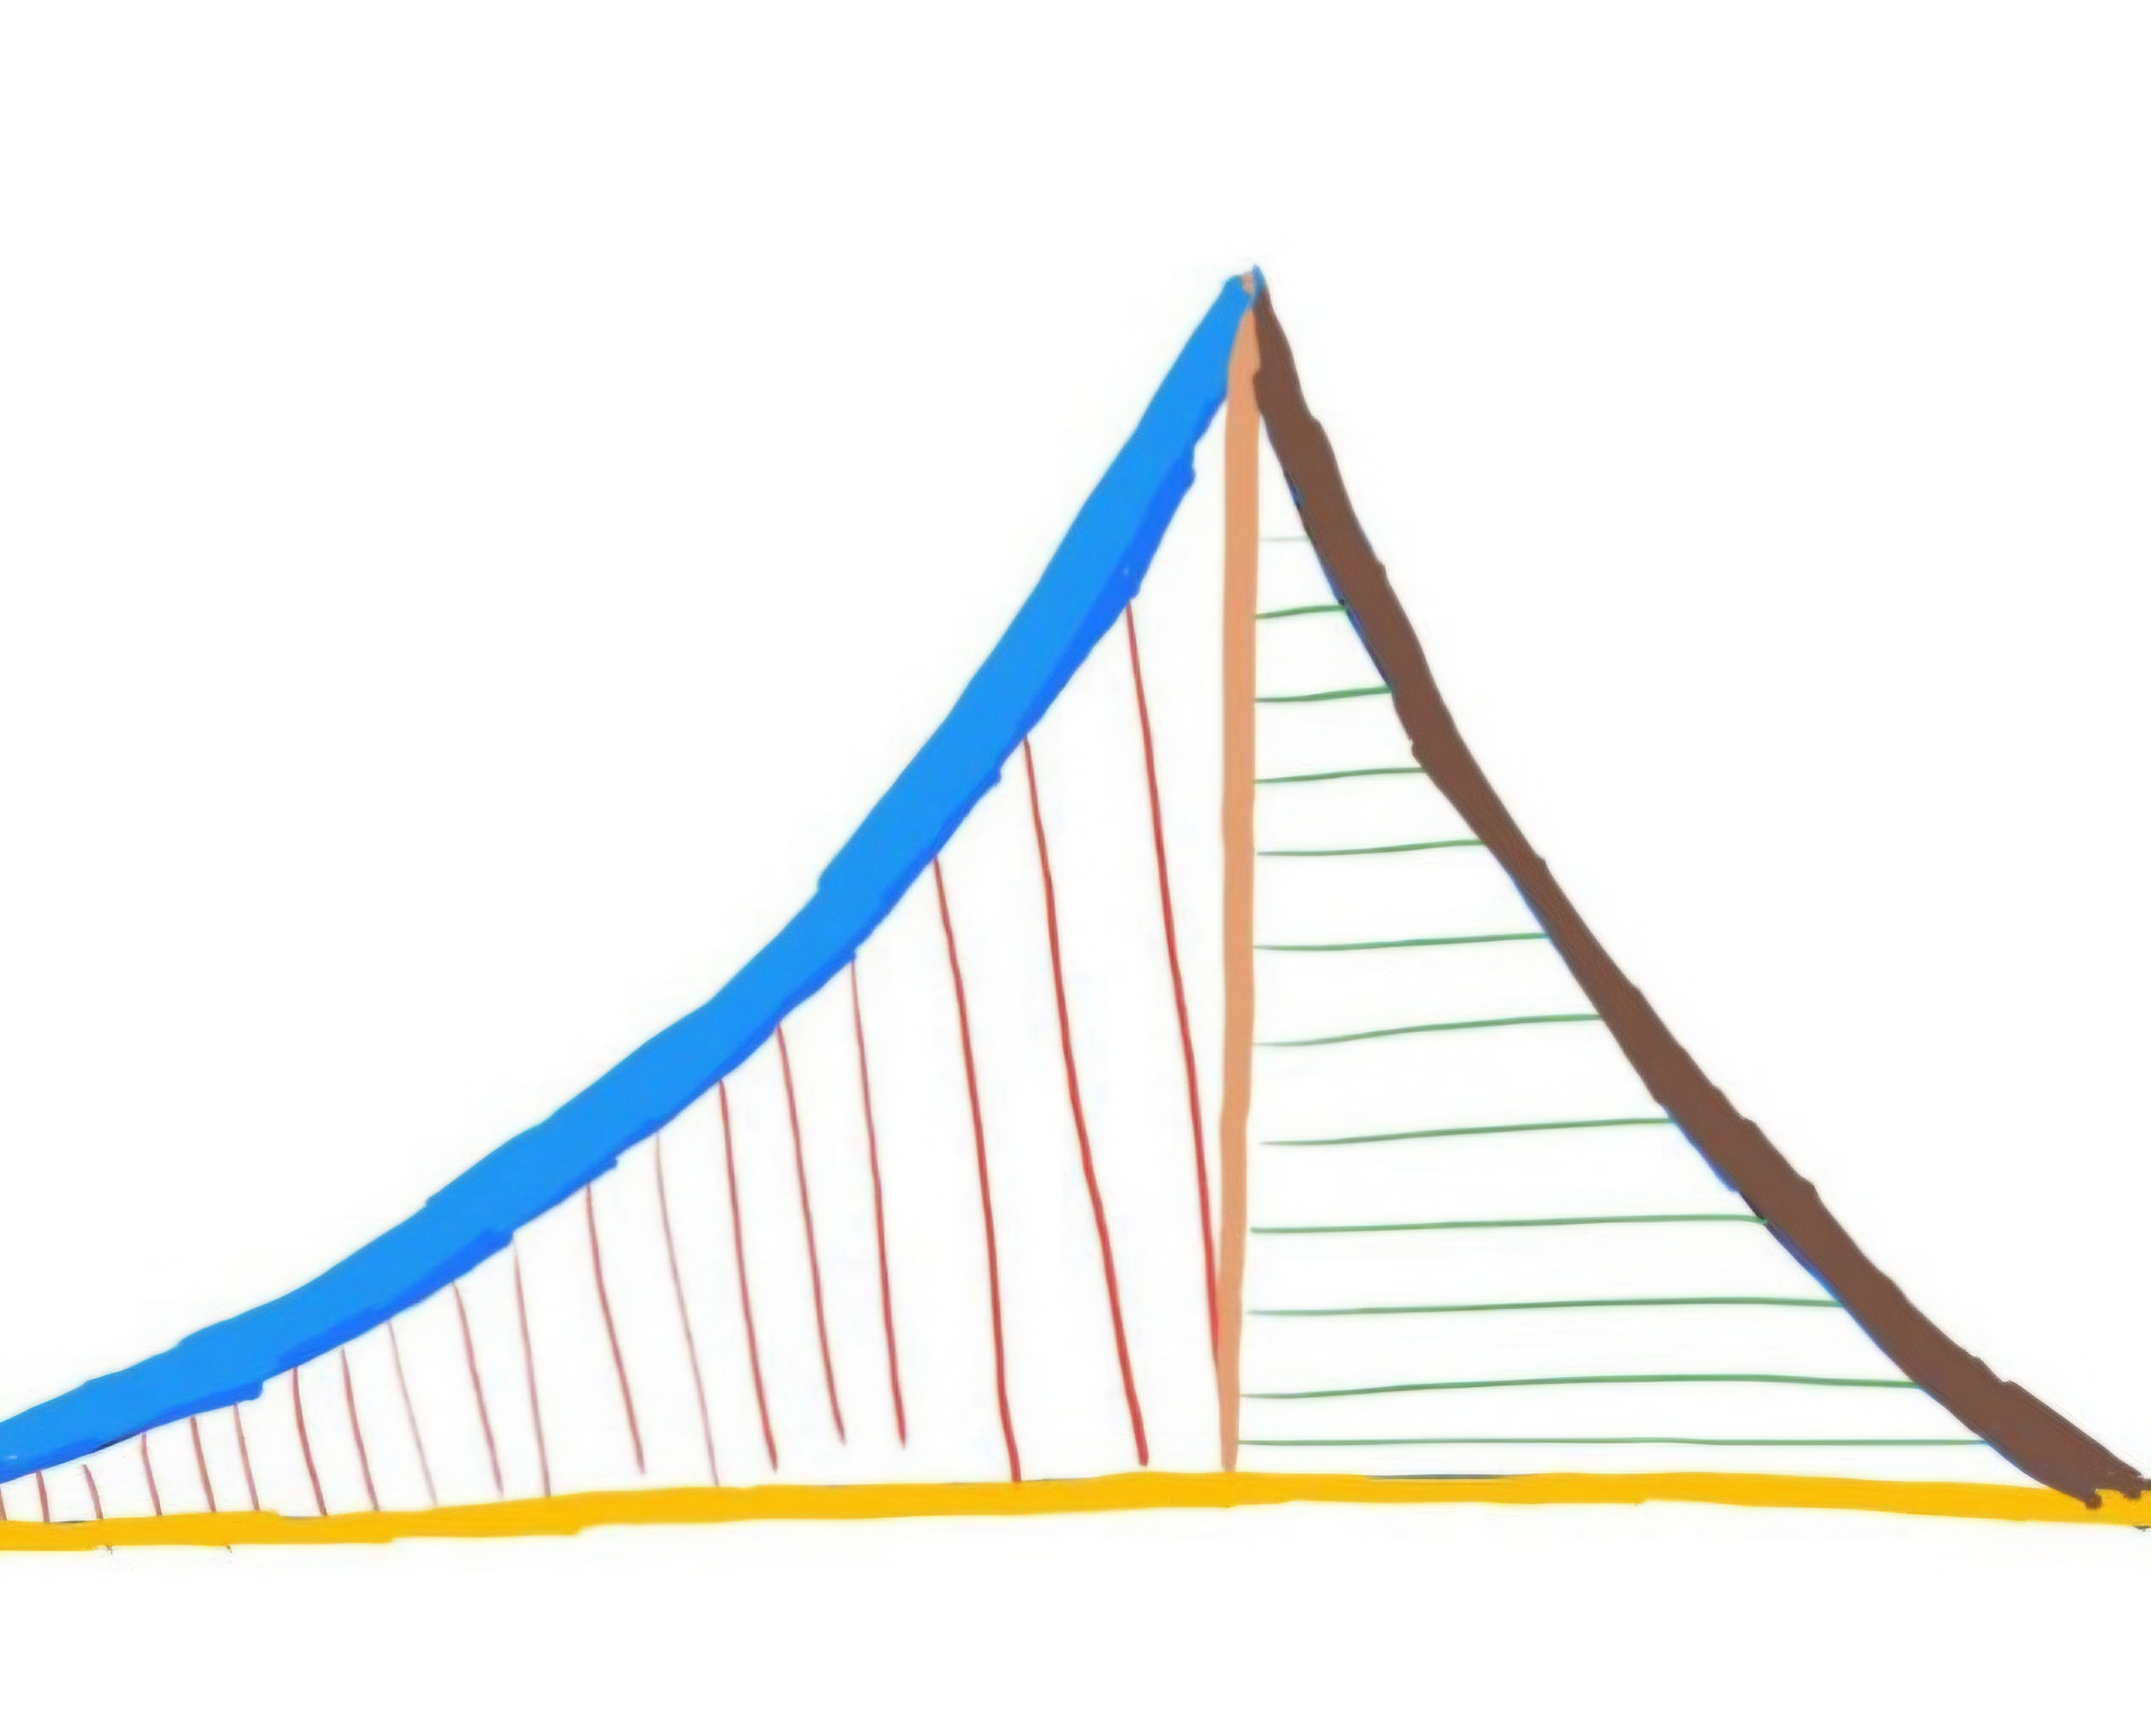
\includegraphics[width=0.2\columnwidth]{figs/logo.jpg}
\\
		{\huge	G. V. V. Sharma}\\Associate Professor,\\Department of Electrical Engineering, \\ IIT Hyderabad
	\end{center}
	%\end{flushleft}
%\IEEEpubid{\makebox[\columnwidth]{978-1-7281-5966-1/20/\$31.00 ©2020 IEEE \hfill} \hspace{\columnsep}\makebox[\columnwidth]{ }}
}
\maketitle

\newpage
\section*{About this Book}

This book introduces progressions, binomial theorem, limits and sequences. 
 All problems in the book are from NCERT mathematics textbooks from Class 9-12.  Exercises are from CBSE, JEE and Olympiad exam papers.   

There is no copyright, so readers are free to print and share.  

%This book is dedicated to my Hindi teacher in school, Shri Mandavi.
\begin{flushright}
\today
\end{flushright}
Github: https://github.com/gadepall/algebra
		\\
License: https://creativecommons.org/licenses/by-sa/3.0/
\\
and
\\
https://www.gnu.org/licenses/fdl-1.3.en.html

\newpage


\tableofcontents

\newpage
%\twocolumn
\onecolumn


%\renewcommand{\theequation}{\theenumi}
\numberwithin{equation}{enumi}
%\numberwithin{figure}{enumi}
\numberwithin{figure}{subsection}
%\renewcommand{\thefigure}{\theenumi}
\renewcommand{\thetable}{\theenumi}

\section{Arithmetic Progression}
\subsection{Formulae}
\begin{enumerate}[label=\thesubsection.\arabic*,ref=\thesubsection.\theenumi]
	\item Find the sum
\begin{align}
	\label{eq:ap-sum10}
	S = 1 + 2 + \dots + 10
\end{align}
\solution Reversing the sum in
	\eqref{eq:ap-sum10}
	as
\begin{align}
	\label{eq:ap-sum10-rev}
	S = 10 + 9 + \dots + 1
\end{align}
and adding 
	\eqref{eq:ap-sum10}
	and
	\eqref{eq:ap-sum10-rev},
\begin{align}
	\label{eq:ap-sum10-add}
	2S &= 11 + 11 + \dots + 11 \quad 10 \text{ times}
	\\
	\implies S &= \frac{11 \times 10}{2} = 55
\end{align}
\item The sum of the first $n$ natural numbers is
\begin{align}
	S_n &= \sum_{k=1}^{n}k = 1+ 2 + \dots + n
	\\
	&= \frac{n\brak{n+1}}{2}
	\label{eq:ap-sumn}
\end{align}
\item The $n$th term of an arithmetic progression (AP) is
\begin{align}
	\label{eq:ap-nthterm}
	a_n = a_0 + nd, \quad n = 0, 1, \dots
\end{align}
\item The sum to $n+1$ terms of an AP is given by
\begin{align}
	\label{eq:ap-nsum}
	S_n &= \sum_{k=0}^{n}a_k = \frac{n+1}{2}\sbrak{a_0 + \frac{dn}{2}}
\end{align}
\solution
From
	\eqref{eq:ap-nthterm}
	and
	\eqref{eq:ap-nsum},
\begin{align}
	\label{eq:ap-nthsum}
	S_n &= \sum_{k=0}^{n}a_k = 
\sum_{k=0}^{n}
	 \brak{a_0 + kd} 
	 \\
	 &= 
\sum_{k=0}^{n}a_0 + 
d\sum_{k=1}^{n}k
	  = \brak{n+1}a_0 + d\frac{n\brak{n+1}}{2}
\end{align}
upon substituting from
	\eqref{eq:ap-sumn}, yielding
	\eqref{eq:ap-nthsum}
	upon simplification.
\end{enumerate}

\subsection{NCERT}
\begin{enumerate}[label=\thesubsection.\arabic*, ref=\thesubsection.\theenumi]
%
\item For the AP 
$$\frac{3}{2}, \frac{1}{2}, -\frac{1}{2}, -\frac{3}{2}, \dots $$ write the first term $a$ and the common difference $d$.
\item Which of the following list of numbers form an AP? If they form an AP, 
write the next two terms 
		\begin{multicols}{2}
\begin{enumerate}
\item $4, 10, 16, 22, \dots$ 
\item $1, -1, -3, -5, \dots$ 
\item $-2, 2, -2, 2, -2, \dots$
\item $1, 1, 1, 2, 2, 2, 3, 3, 3, \dots$
\end{enumerate}
\end{multicols}
\item Find the 10th term of the AP : $2,  7,  12,  \dots$
\item Which term of the AP : $21,  18,  15,  \dots$ is - 81? Also,  is any term 0? Give reason for your answer.
\item Determine the AP whose 3rd term is 5 and the 7th term is 9.
\item Check whether 301 is a term of the list of numbers $5,  11,  17,  23,  \dots$
\item How many two-digit numbers are divisible by 3?
\item Find the 11th term from the last term (towards the first term) of the
AP : $10,  7,  4,  \dots,  - 62$.
\item A sum of \rupee 1000 is invested at $8\%$ simple interest per year. Calculate the interest at the end of each year. Do these interests form an AP? If so,  find the interest at the end of 30 years making use of this fact.
\item In a flower bed,  there are 23 rose plants in the first row,  21 in the
second,  19 in the third,  and so on. There are 5 rose plants in the last row. How many rows are there in the flower bed?
\item Find the sum of the first 22 terms of the AP : $8,  3,  -2,  \dots$
\item If the sum of the first 14 terms of an AP is 1050 and its first term is 10,  find the 20th term.
\item How many terms of the AP : $24,  21,  18,  \dots$ must be taken so that their
sum is 78?
\item Find the sum of 
\begin{enumerate}
\item the first 1000 positive integers.
\item the first $n$ positive integers.
\end{enumerate}
\item Find the sum of first 24 terms of the list of numbers whose $n^{th}$ term is given by $a_n = 3 + 2n$
\item A manufacturer of TV sets produced 600 sets in the third year and 700
sets in the seventh year. Assuming that the production increases uniformly by a fixed number every year,  find 
\begin{enumerate}
\item   the production in the 1st year
\item	the production in the 10th year
\item the total production in first 7 years.
\end{enumerate}
\item In which of the following situations,  does the list of numbers involved make an arithmetic progression,  and why?
\begin{enumerate}
\item The taxi fare after each km when the fare is \rupee 15 for the first km and \rupee 8 for each additional km.
\item The amount of air present in a cylinder when a vacuum pump removes 
$\frac{1}{4}$ of the air remaining in the cylinder at a time.
\item  The cost of digging a well after every metre of digging,  when it costs \rupee 150 for the first metre and rises by \rupee 50 for each subsequent metre.
\item The amount of money in the account every year,  when \rupee 10000 is deposited at compound interest at 8 \% per annum.
\end{enumerate}
\item Write first four terms of the AP,  when the first term $a$ and the common difference $d$ are
given as follows
		\begin{multicols}{2}
\begin{enumerate}
\item $a = 10,  d = 10	$	
\item $a = 4,  d = -3	$	
\item $a = -2,  d = 0	$	
\item $ a = -1,  d =\frac{1}{2}$
\item $a = -1.25,  d = -0.25$	
\end{enumerate}
\end{multicols}
\item For the following APs,  write the first term and the common difference
	\begin{multicols}{2}
		\begin{enumerate}[itemsep=1ex]
\item $3,  1,  -1,  -3,  \dots $
\item $-5,  -1,  3,  7,  \dots $
\item $\frac{1}{3},  \frac{5}{3},  \frac{9}{3},  \frac{13}{3}, \dots $
\item $0.6,  1.7,  2.8,  3.9, \dots $ 
\end{enumerate}
\end{multicols}
\item Which of the following are APs? If they form an AP,  find the common difference $d$ and
write three more terms.
\begin{multicols}{2}
\begin{enumerate}[itemsep=1ex]
\item $2,  4,  8,  16,  \dots $
\item $2, \frac{5}{2},  3,  \frac{7}{2}, \dots $
\item $-1.2,  -3.2,  -5.2,  -7.2,  \dots $
\item $-10,  -6,  -2,  2,  \dots $
\item $3, 3+\sqrt{2},  3+2\sqrt{2},  3+3\sqrt{2}, \dots $
\item $0.2,  0.22,  0.222,  0.2222,  \dots $
\item $0,  -4,  -8,  -12,  \dots $
\item $-\frac{1}{2},  -\frac{1}{2},  -\frac{1}{2},  -\frac{1}{2}, \dots $
\item $1,  3,  9,  27, \dots $ 
\item $a,  2a,  3a,  4a, \dots $ 
\item $a,  a^2,  a^3,  a^4, \dots $
\item $\sqrt{2},  \sqrt{8},  \sqrt{18},  \sqrt{32}, \dots $
\item $\sqrt{3},  \sqrt{6},  \sqrt{9},  \sqrt{12}, \dots $
\item $1^2,  3^2,  5^2,  7^2, \dots$
\item $1^2,  5^2,  7^2,  73, \dots $
\end{enumerate}
\end{multicols}
\item Fill in the blanks in 
	\tabref{table:ap},  given that $a$ is the first term,  $d$ the common
difference and $a_n$ the $n^{th}$ term of the AP.
\begin{table}[H]
	\centering
\begin{tabular}{|c|c|r|l|l|}
\hline
\\
&$a$& $d$ & $n$ & $a_n$
\\
\hline
(i)& 	7 &3 &8 &$\dots $ 
\\
(ii)& 	-18 &$\dots $  &10  &0
\\
(iii)& 	$\dots $  &-3 &18 &-5
\\
(iv)& 	-18.9 &2.5 &$\dots $  &3.6
\\
(v)& 	3.5 &0 &105 &$\dots $ 
\\
\hline
\end{tabular}
	\caption{}
	\label{table:ap}
\end{table}
\item Choose the correct choice in the following and justify 
\begin{enumerate}
	\item $30^{th}$ term of the AP: $10,  7,  4, \dots $   is
	\begin{multicols}{4}
\begin{enumerate}
\item 97
\item 77
\item -77
\item -87
\end{enumerate}
\end{multicols}
\item $11^{th}$ term of the AP: $ -3,  -\frac{1}{2},  2, \dots  $ is 
	\begin{multicols}{4}
\begin{enumerate}
\item 28
\item 22
\item -38
\item $-48\frac{1}{2}$
\end{enumerate}
\end{multicols}
\item In the following APs,  find the missing terms in the blanks  
	\begin{multicols}{2}
\begin{enumerate}
\item $2,  \dots,  26$
\item $\dots  ,  13, \dots  ,  3$
\item $5,  \dots  ,  \dots  ,  9\frac{1}{2}$
\item $-4,  \dots  ,  \dots  ,  \dots  ,  \dots,  6$
\item $\dots ,  38,  \dots ,  \dots ,  \dots ,  -22$
\end{enumerate}
\end{multicols}
\end{enumerate}
\item Which term of the AP : $3,  8,  13,  18,  \dots $ is 78?
\item Find the number of terms in each of the following APs:
\begin{enumerate}
	\item $7,  13,  19,  \dots , 205$.
	\item $18,  15\frac{1}{2},  13, \dots , -47$
\end{enumerate}
\item Check whether -150 is a term of the AP : $11,  8,  5,  2 \dots $ 
\item Find the 31st term of an AP whose 11th term is 38 and the 16th term is 73.
\item An AP consists of 50 terms of which 3rd term is 12 and the last term is 106. Find the 29th term.
\item If the 3rd and the 9th terms of an AP are 4 and -8 respectively,  which term of this AP is zero?
\item The 17th term of an AP exceeds its 10th term by 7. Find the common difference.
\item Which term of the AP : $3,  15,  27,  39, \dots $  will be 132 more than its 54th term? 
\item How many three-digit numbers are divisible by 7?
\item How many multiples of 4 lie between 10 and 250?
\item For what value of $n$,  are the $n^{th}$ terms of two APs: $63,  65,  67, \dots $  and $3,  10,  17, \dots $  equal?
\item Determine the AP whose third term is 16 and the 7th term exceeds the 5th term by 12.
\item Find the 20th term from the last term of the AP : $3,  8,  13, \dots  ,  253$.
\item The sum of the 4th and 8th terms of an AP is 24 and the sum of the 6th and 10th terms is 44. Find the first three terms of the AP.
\item Subba Rao started work in 1995 at an annual salary of \rupee 5000 and received an increment of \rupee 200 each year. In which year did his income reach \rupee 7000?
\item Ramkali saved \rupee 5 in the first week of a year and then increased her weekly savings by \rupee 1.75. If in the $n^{th}$ week,  her weekly savings become \rupee 20.75,  find $n$.
\item Find the sum of the following APs
	\begin{multicols}{2}
\begin{enumerate}
	\item $2,  7,  12,  \dots $,  to 10 terms.
	\item $-37,  -33,  -29,  \dots $,  to 12 terms.
	\item $ 0.6,  1.7,  2.8,  \dots $,  to 100 terms.
	\item $\frac{1}{15},  \frac{1}{12},  \frac{1}{10}, \dots  $ to 11 terms.
\end{enumerate}
\end{multicols}
\item Find the sums given below 
\begin{enumerate}
\item $7+10\frac{1}{2}+14+\dots +84$
\item $34 + 32 + 30 + \dots + 10$
\item $-5 + (-8) + (-11) + \dots + (-230)$
\end{enumerate}
\item In an A.P
\begin{enumerate}
\item given $a = 5,  d = 3,  a_n = 50$,  find $n$ and $S_n$.
\item given $a = 7,  a_{13} = 35$,  find $d$ and $S_{13}$.
\item  given $a_{12} = 37,  d = 3$,  find $a$ and $S_{12}$.
\item given $a_3 = 15,  S_{10} = 125$,  find $d$ and $a_{10}$.
\item given $d = 5,  S_9= 75$,  find $a$ and $a_9$.
\item given $a = 2,  d = 8,  S_n = 90$,  find $n$ and $a_n$.
\item  given $a = 8,  a_n = 62,  S_n = 210$,  find $n$ and $d$.
\item given $a_n = 4,  d = 2,  S_n = -14$,  find $n$ and $a$.
\item given $a = 3,  n = 8,  S = 192$,  find $d$.
\item given $l = 28,  S = 144$,  and there are total 9 terms. Find $a$.
\end{enumerate}
\item How many terms of the AP : $9,  17,  25,  \dots $ must be taken to give a sum of 636?
\item The first term of an AP is 5,  the last term is 45 and the sum is 400. Find the number of terms and the common difference.
\item The first and the last terms of an AP are 17 and 350 respectively. If the common difference is 9,  how many terms are there and what is their sum?
\item Find the sum of first 22 terms of an AP in which d = 7 and 22nd term is 149.
\item Find the sum of first 51 terms of an AP whose second and third terms are 14 and 18 respectively.
\item If the sum of first 7 terms of an AP is 49 and that of 17 terms is 289,  find the sum of first $n$ terms. 
\item Show that $a_1 ,  a_2 ,  \dots,  a_n,  \dots$  form an AP where $a_n$ is defined as below 
\begin{enumerate}
	\item $a_n = 3 + 4n$
	\item $a_n = 9 - 5n$
\end{enumerate}
Also find the sum of the first 15 terms in each case.
\item If the sum of the first $n$ terms of an AP is $4n - n^2$,  what is the first term (that is $S_1$ )? What
is the sum of first two terms? What is the second term? Similarly,  find the 3rd,  the 10th and
the $n$th terms.
\item Find the sum of the first 40 positive integers divisible by 6.
\item Find the sum of the first 15 multiples of 8.
\item Find the sum of the odd numbers between 0 and 50.
\item A contract on construction job specifies a penalty for delay of completion beyond a
certain date as follows: \rupee 200 for the first day, \rupee 250 for the second day,  \rupee 300 for the third
day,  etc.,  the penalty for each succeeding day being \rupee 50 more than for the preceding day. How much money the contractor has to pay as penalty,  if he has delayed the work by 30 days?
\item A sum of \rupee 700 is to be used to give seven cash prizes to students of a school for their overall academic performance. If each prize is \rupee 20 less than its preceding prize,  find the value of each of the prizes.
\item  In a school,  students thought of planting trees in and around the school to reduce air pollution. It was decided that the number of trees,  that each section of each class will plant,  will be the same as the class,  in which they are studying,  
e.g.,  a section of Class I will plant 1 tree,  
a section of Class II will plant 2 trees and so on till Class XII. There are three sections of each class. How many trees will be planted by the students?
\item A spiral is made up of successive semicircles,  with centres alternately at A and B,  starting with centre at A,  of radii $0.5 cm,  1.0 cm,  1.5 cm,  2.0 cm, \dots $  as shown in Fig.
		\ref{fig:fig}
	What is the total length of such a spiral made up of thirteen consecutive 22 semicircles? (Take $\pi =\frac{22}{7}$)
	\begin{figure}[H]
		\centering
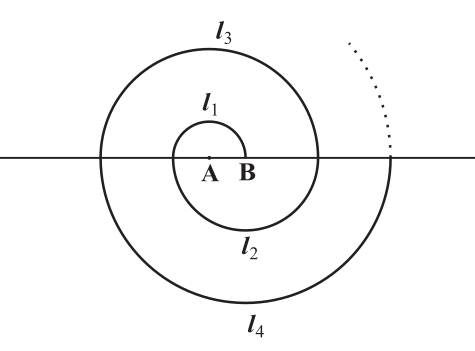
\includegraphics[width=0.75\columnwidth]{figs/ap/fig.png} 
		\caption{}
		\label{fig:fig}
	\end{figure}
{\em Hint:} Length of successive semicircles is $l_1,  l_2,  l_3,  l_4 ,  \dots$ with centres at A,  B,  A,  B,  $\dots $, respectively.
\item 200 logs are stacked in the following manner: 20 logs in the bottom row,  19 in the next row,  18 in the row next to it and so on (see Fig
		\ref{fig:fig1}
	). In how many rows are the 200 logs placed and how many logs are in the top row?
	\begin{figure}[H]
		\centering
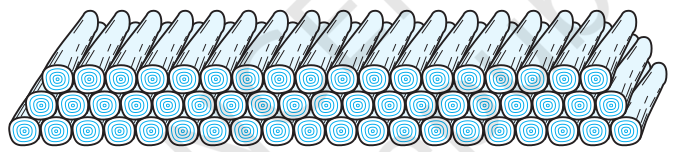
\includegraphics[width=0.75\columnwidth]{figs/ap/fig1.png}
		\caption{}
		\label{fig:fig1}
	\end{figure}
\item In a potato race,  a bucket is placed at the starting point,  which is $5m$ from the first potato,  and the other potatoes are placed $3m$ apart in a straight line. There are ten potatoes in the line
		as shown in \figref{fig:fig3}.
	\begin{figure}[H]
		\centering
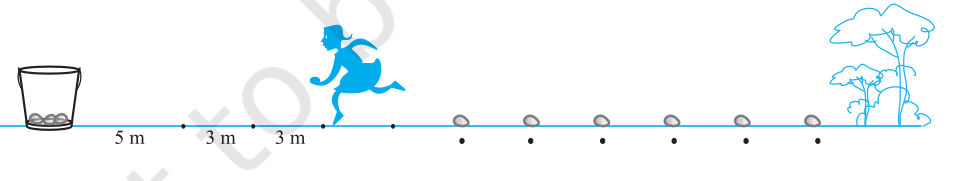
\includegraphics[width=0.75\columnwidth]{figs/ap/fig3.png} 
		\caption{}
		\label{fig:fig3}
	\end{figure}
A competitor starts from the bucket,  picks up the nearest potato,  runs back with it,  drops it in the bucket,  runs back to pick up the next potato,  runs to the bucket to drop it in,  and she continues in the same way until all the potatoes are in the bucket. What is the total distance the competitor has to run?\
[{\em Hint:} To pick up the first potato and the second potato,  the total distance (in metres)
run by a competitor is $2 \times 5 + 2 \times (5 + 3)$].
\item Which term of the AP : $121,  117,  113, \dots $ is its first negative term? [{\em Hint:} Find $n$ for $a_n < 0$]
\item The sum of the third and the seventh terms of an AP is 6 and their product is 8. Find the sum of first sixteen terms of the AP.
\item The houses of a row are numbered consecutively from 1 to 49. Show that there is a value of $x$ such that the sum of the numbers of the houses preceding the house numbered $x$ is equal to the sum of the numbers of the houses following it. Find this value of $x$.[{\em Hint:} $S_{x-1} = S_{49} -S_x$]
\item A small terrace at a football ground comprises of 15 steps each of which is $50 m$ long and built of solid concrete. Each step has rise of $\frac{1}{4}m$ and a tread of $\frac{1}{2}m$ 
	(see \figref{fig:fig5}).
	Calculate the total volume of concrete required to build the terrace. [{\em Hint:} Volume of concrete required to build the first step = $\frac{1}{4} \times \frac{1}{2} \times 50m^3$]
	\begin{figure}[H]
		\centering
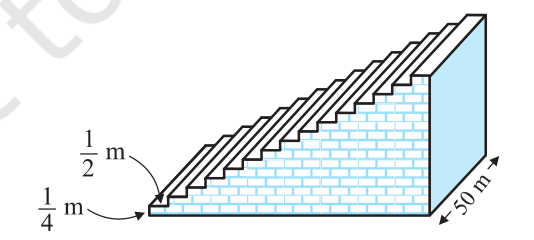
\includegraphics[width=0.75\columnwidth]{figs/ap/fig5.png}  
		\caption{}
		\label{fig:fig5}
	\end{figure}
\item Find the sum to $n$ terms of the following series
	\begin{multicols}{4}
\begin{enumerate}
	\item $a_n =2n+5$
	\item $a_n =\frac{n-3}{4}$
\item $a_n = \frac{2n-3}{6}$
\item $a_n = 4n-3 $
\end{enumerate}
\end{multicols}
\item Find the sum of all natural numbers lying between 100 and 1000,  which are multiples of 5.
\item In an AP,  the first term is 2 and the sum of the first five terms is one-fourth of the next five terms. Show that $20^{th}$ term is -112.
\item How many terms of the AP  $-6, -\frac{11}{2},  -5, \dots $ are needed to give the sum -25?
\item In an AP,  If $p^{th}$ term is $\frac{1}{q}, q^{th}$ term is $\frac{1}{p}$,  prove that the sum of first $pq$ terms is $\frac{1}{2}(pq+1)$,  where $p \neq q.$
\item  If the sum of a certain number of terms of the AP: $25,  22,  19,  \dots $  is 116, find the last term.
\item Find the sum to $n$ terms of the AP,  whose $k^{th}$ term is $5k + 1$.
\item If the sum of $n$ terms of an AP is $pn + qn^2$,  where $p$ and $q$ are constants,  find the common difference.
\item The sums of $n$ terms of two arithmetic progressions are in the ratio $5n + 4 : 9n + 6$. Find the ratio of their $18^{th}$ terms.
\item If the sum of first $p$ terms of an AP is equal to the sum of the first $q$ terms,  then find the sum of the first $p + q$ terms.
\item Sum of the first $p,  q$ and $r$ terms of an AP are $a,  b$ and $c$,  respectively. Prove that
$$\frac{a}{p}(q-r)+\frac{b}{q}(r-p)+\frac{c}{r}(p-q) = 0$$
\item The ratio of the sums of $m$ and $n$ terms of an AP is $m^2 : n^2$. Show that the ratio of 
$m^{th}$ and $n^{th}$ term is $(2m - 1) : (2n - 1)$.
\item If the sum of $n$ terms of an AP is $3n^2 + 5n$ and its $m^{th}$ term is 164,  find the value
of $m$.
\item Insert five numbers between 8 and 26 such that the resulting sequence is an AP
\item Between 1 and 31,  $m$ numbers have been inserted in such a way that the resulting sequence is an AP and the ratio of $7^{th}$ and $(m - 1)^{th}$ numbers is 5 : 9. Find the value of $m$.
\item A man starts repaying a loan as first instalment of \rupee 100. If he increases the
instalment by Rs 5 every month,  what amount he will pay in the $30^{th}$ instalment?
\item The difference between any two consecutive interior angles of a polygon is 5$\degree$. If the smallest angle is 120$\degree$,  find the number of the sides of the polygon. 
\item Show that the sum of $(m + n)^{th}$ and $(m - n)^{th}$ terms of an AP is equal to twice the $m^{th}$ term.
\item If the sum of three numbers in AP  is 24 and their product is 440,  find the numbers.
\item Let the sum of $n,  2n,  3n$ terms of an AP be $S_1,  S_2$ and $S_3$,  respectively,  show that 
$$S_3 = 3(S_2 - S_1)$$
\item Find the sum of all numbers between 200 and 400 which are divisible by 7.
\item Find the sum of integers from 1 to 100 that are divisible by 2 or 5.
\item  The sum of the first four terms of an AP  is 56. The sum of the last four terms is 112. If its first term is 11, then find the number of terms.
\item The $p^{th}, q^{th}$ and $r^{th}$ terms of an AP  are $a, b, c,$ respectively. Show that 
$$\brak{q - r }a + \brak{r - p }b + \brak{p - q }c = 0.$$
\item If $$a\brak{\frac{1}{b}+\frac{1}{c}}, b\brak{\frac{1}{c}+\frac{1}{a}}, c\brak{\frac{1}{a}+\frac{1}{b}}$$ are in AP, prove that $a, b, c$ are in AP. 
\item In an AP if the $m^{th}$ is $n$ and the $n^{th}$ term is $m$, where $m \ne n$, find the $p^{th}$ term.
\item If the sum of $n$ terms of an AP is
	$$nP+\frac{1}{2} n\brak{n-1}Q,$$
	where $P$ and $Q$ are constants, find the common difference.
\item The sum of $n$ terms of two arithmetic progressions are in the ratio
	$\brak{3n+8}:\brak{7n+15}$.  Find the ratio of their $12^{th}$ terms.
\item The income of a person is \rupee 3,00,000 in the first year and he receives an increase of \rupee 10,000 to his income per year for the next 19 years.  Find the total amount he received in 20 years.
\item Insert 6 numbers between 3 and 24 such that the resulting sequence is an AP.
\item Two APs have the same common difference. The difference between their 100th terms is 100,  what is the difference between their 1000th terms?
\item Find the sum of odd integers from 1 to 2001.
\item If $\frac{a^n+b^n}{a^{n-1}+b^{n-1}}$ is the AM  between $a$ and $b$,  then find the value of $n$.
\item Find the sum of all two digit numbers which when divided by 4,  yields 1 as remainder.
\item A farmer buys a used tractor for Rs 12000. He pays Rs 6000 cash and agrees to pay the balance in annual instalments of Rs 500 plus 12\% interest on the unpaid amount. How much will the tractor cost him?
\item Shyam Anand buys a scooter for Rs 22000. He pays Rs 4000 cash and agrees to
pay the balance in annual instalment of Rs 1000 plus 10\% interest on the unpaid
amount. How much will the scooter cost him?
\item A man deposited Rs 10000 in a bank at the rate of 5\% simple interest annually. Find the amount in the $15^{th}$ year since he deposited the amount and also calculate the total amount after 20 years.

\end{enumerate}

\section{Geometric Progression}
\subsection{Formulae}
%\begin{enumerate}[label=\thesubsection.\arabic*.,ref=\thesubsection.\theenumi]
\item Find the $20^{th}$ and $n^{th}$ terms of the GP: $\frac{5}{2}, \frac{5}{4}, \frac{5}{8},\dots, $
\item Find the $12^{th}$ term of a GP  whose $8^{th}$ term is 192 and the common ratio is 2.
\item The $5^{th}$, $8^{th}$ and $11^{th}$ terms of a GP  are $p, q$ and $s$, respectively. Show that 
$q^2 = ps$.
\item The $4^{th}$ term of a GP  is square of its second term, and the first term is -3. Determine its $7^{th}$ term.
\item Find the sum to $n$ terms of the following series
\begin{enumerate}
\item $a_n = 2^n$
\item $n^2 + 2^n$
\end{enumerate}
\item Which term of the following sequences
\begin{enumerate}
	\item 2, 2, $\sqrt{2}$, 4,\dots,  is 128 ?
	\item $\sqrt{3}, 3, 3\sqrt{3},\dots,$  is 729?
	\item $\frac{1}{3}, \frac{1}{9}, \frac{1}{27}, \dots,$  is $\frac{1}{19683}$?
\end{enumerate}
\item For what values of $x$, the numbers $-\frac{2}{7}, x, -\frac{7}{2}$ are in GP?
\\
	Find the sum to indicated number of terms in each of the geometric progressions.
\item 0.15, 0.015, 0.0015,\dots,  20 terms.
\item $\sqrt{7}, \sqrt{21}, \sqrt[3]{7}, \dots,  n$ terms.
\item $1, -a, a^2, -a^2, a^3,\dots,  n$ terms $\brak{a \neq -1}$.
\item $x^3, x^5, x^7,\dots,  n$ terms $\brak{x \neq \pm 1}$.
\item Evaluate $$\sum _{k=1}^{11} \brak{2 + 3^k}.$$
\item The sum of first three terms of a GP  is $\frac{39}{10}$ and their product is 1. Find the 10
common ratio and the terms.
\item How many terms of GP  3, $3^2, 3^3$, \dots,  are needed to give the sum 120?
\item The sum of first three terms of a GP  is 16 and the sum of the next three terms is 128. Determine the first term, the common ratio and the sum to n terms of the GP 
\item Given a GP  with $a = 729$ and $7^{th}$ term 64, determine $S_7$.
\item Find a GP  for which sum of the first two terms is -4 and the fifth term is 4 times the third term.
\item If the $4^{th}$, $10^{th}$ and $16^{th}$ terms of a GP  are $x, y$ and $z$, respectively. Prove that $x, y, z$ are in GP.
\item Find the sum to $n$ terms of the sequence, $8, 88, 888, 8888, \dots$. 
\item Find the sum of the products of the corresponding terms of the sequences 2, 4, 8, 16, 32, and 128, 32, 8, 2, $\frac{1}{2}$.
\item Show that the products of the corresponding terms of the sequences $a, ar, ar^2,\dots,  ar^{n-1}$ and $A, AR, AR^2,\dots,  AR^{n -1}$ form a GP  and find the common ratio.
\item Find four numbers forming a geometric progression in which the third term is greater than the first term by 9, and the second term is greater than the $4^{th}$ by 18.
\item If the $p^{th}, q^{th}$ and $r^{th}$ terms of a GP  are $a, b$ and $c$, respectively. Prove that 
$$a^{q-r} b^{r-p} c^{p-q} = 1.$$
\item If the first and the $n^{th}$ term of a GP  are $a$ and $b$, respectively, and if $P$ is the product of $n$ terms, prove that $P^2 = \brak{ab}^n.$
\item Show that the ratio of the sum of first $n$ terms of a GP  to the sum of terms from $\brak{n+1}^{th}$ to $\brak{2n}^{th}$ term is $\frac{1}{r^n}$.
\item If $a, b, c$ and $d$ are in GP  show that $\brak{a^2 + b^2 + c^2}\brak{b^2 + c^2 + d^2} = \brak{ab + bc + cd}^2.$
\item Insert two numbers between 3 and 81 so that the resulting sequence is GP 
\item Find the value of $n$ so that $$\frac{a^{n + 1} + b^{n + 1}}{a^n + b^n}$$ may be the geometric mean between $a$ and $b$.
\item The sum of two numbers is 6 times their geometric mean, show that numbers are in the ratio $$\brak{3+2\sqrt{2}}:\brak{3-2\sqrt{2}}.$$
\item If $A$ and $G$ be AM  and GM , respectively between two positive numbers, prove that the numbers are $$AP  \sqrt{\brak{A+G}\brak{A-G}}.$$
\item The number of bacteria in a certain culture doubles every hour. If there were 30 bacteriAP esent in the culture originally, how many bacteria will be present at the end of $2^{nd}$ hour, 
$4^{th}$ hour and $n^{th}$ hour ?
\item What will Rs 500 amount to in 10 years after its deposit in a bank which pays annual interest rate of 10\% compounded annually?
\item If AM  and GM  of roots of a quadratic equation are 8 and 5, respectively, then obtain the quadratic equation.
\item If $f$ is a function satisfying $$f\brak{x +y} = f\brak{x} f\brak{y} \forall x,y \in N$$ such that 
	$$f\brak{1} = 3\text{ and }\sum_{x = 1}^n f\brak{x} = 120,$$ find the value of $n$.
\item The sum of some terms of GP  is 315 whose first term and the common ratio are 5 and 2, respectively. Find the last term and the number of terms.
\item  The first term of a GP  is 1. The sum of the third term and fifth term is 90. Find the common ratio of the GP.
\item The sum of three numbers in GP  is 56. If we subtract 1, 7, 21 from these numbers in that order, we obtain an arithmetic progression. Find the numbers.
\item A GP  consists of an even number of terms. If the sum of all the terms is 5 times the sum of terms occupying odd places, then find its common ratio.
\item  The sum of the first four terms of an AP  is 56. The sum of the last four terms is 112. If its first term is 11, then find the number of terms.
\item If $$\frac{a+bx}{a-bx} = \frac{b+cx}{b-cx} = \frac{c+dx}{c-dx}\brak{x \neq 0},$$ then show that $a, b, c$ and $d$ are in GP.
\item Let $S$ be the sum, $P$ the product and $R$ the sum of reciprocals of $n$ terms in a GP.  Prove that $P^2R^n = S^n.$ 
\item The $p^{th}, q^{th}$ and $r^{th}$ terms of an AP  are $a, b, c,$ respectively. Show that 
$$\brak{q - r }a + \brak{r - p }b + \brak{p - q }c = 0.$$
\item If $$a\brak{\frac{1}{b}+\frac{1}{c}}, b\brak{\frac{1}{c}+\frac{1}{a}}, c\brak{\frac{1}{a}+\frac{1}{b}}$$ are in AP, prove that $a, b, c$ are in AP 
\item If $a, b, c, d$ are in GP  prove that $$\brak{a^n + b^n}, \brak{b^n + c^n}, \brak{c^n + d^n}$$ are in GP. 
\item If $a$ and $b$ are the roots of $$x^2 - 3x + p = 0$$ and $c, d$ are roots of $$x^2 - 12x + q = 0,$$ where $a, b, c, d$ form a GP,  prove that $$\brak{q + p} : \brak{q - p} = 17:15.$$
\item The ratio of the AM  and GM  of two positive numbers $a$ and $b$, is $m : n$. Show that 
$$a:b = \brak{m+\sqrt{m^2 - n^2}}:\brak{m - \sqrt{m^2 - n^2}}.$$
\item If $a, b, c$ are in AP; $b, c, d$ are in GP  and $$\frac{1}{c}, \frac{1}{d}, \frac{1}{e}$$ are in AP  prove that $a, c, e$ are in GP.
\item Find the sum of the following series up to $n$ terms
\begin{enumerate}
\item 5 + 55 +555 + \dots, 
\item .6 + .66 + .666+\dots 
\end{enumerate}
\item Find the $20^{th}$ term of the series $$2 \times 4 + 4 \times 6 + 6 \times 8 + \dots  $$ 
\item Find the sum of the first $n$ terms of the series: 3 + 7 + 13 + 21 + 31 + \dots, 
\item If $S_1, S_2, S_3$ are the sum of first n natural numbers, their squares and their cubes, respectively, show that $$9 S_2^2 = S_3 \brak{1 + 8S_1}.$$
\end{enumerate}

\subsection{NCERT}
\begin{enumerate}[label=\thesubsection.\arabic*.,ref=\thesubsection.\theenumi]
\item Find the $20^{th}$ and $n^{th}$ terms of the GP: $\frac{5}{2}, \frac{5}{4}, \frac{5}{8},\dots, $
\item Find the $12^{th}$ term of a GP  whose $8^{th}$ term is 192 and the common ratio is 2.
\item The $5^{th}$, $8^{th}$ and $11^{th}$ terms of a GP  are $p, q$ and $s$, respectively. Show that 
$q^2 = ps$.
\item The $4^{th}$ term of a GP  is square of its second term, and the first term is -3. Determine its $7^{th}$ term.
\item Find the sum to $n$ terms of the following series
\begin{enumerate}
\item $a_n = 2^n$
\item $n^2 + 2^n$
\end{enumerate}
\item Which term of the following sequences
\begin{enumerate}
	\item 2, 2, $\sqrt{2}$, 4,\dots,  is 128 ?
	\item $\sqrt{3}, 3, 3\sqrt{3},\dots,$  is 729?
	\item $\frac{1}{3}, \frac{1}{9}, \frac{1}{27}, \dots,$  is $\frac{1}{19683}$?
\end{enumerate}
\item For what values of $x$, the numbers $-\frac{2}{7}, x, -\frac{7}{2}$ are in GP?
\\
	Find the sum to indicated number of terms in each of the geometric progressions.
\item 0.15, 0.015, 0.0015,\dots,  20 terms.
\item $\sqrt{7}, \sqrt{21}, \sqrt[3]{7}, \dots,  n$ terms.
\item $1, -a, a^2, -a^2, a^3,\dots,  n$ terms $\brak{a \neq -1}$.
\item $x^3, x^5, x^7,\dots,  n$ terms $\brak{x \neq \pm 1}$.
\item Evaluate $$\sum _{k=1}^{11} \brak{2 + 3^k}.$$
\item The sum of first three terms of a GP  is $\frac{39}{10}$ and their product is 1. Find the 10
common ratio and the terms.
\item How many terms of GP  3, $3^2, 3^3$, \dots,  are needed to give the sum 120?
\item The sum of first three terms of a GP  is 16 and the sum of the next three terms is 128. Determine the first term, the common ratio and the sum to n terms of the GP 
\item Given a GP  with $a = 729$ and $7^{th}$ term 64, determine $S_7$.
\item Find a GP  for which sum of the first two terms is -4 and the fifth term is 4 times the third term.
\item If the $4^{th}$, $10^{th}$ and $16^{th}$ terms of a GP  are $x, y$ and $z$, respectively. Prove that $x, y, z$ are in GP.
\item Find the sum to $n$ terms of the sequence, $8, 88, 888, 8888, \dots$. 
\item Find the sum of the products of the corresponding terms of the sequences 2, 4, 8, 16, 32, and 128, 32, 8, 2, $\frac{1}{2}$.
\item Show that the products of the corresponding terms of the sequences $a, ar, ar^2,\dots,  ar^{n-1}$ and $A, AR, AR^2,\dots,  AR^{n -1}$ form a GP  and find the common ratio.
\item Find four numbers forming a geometric progression in which the third term is greater than the first term by 9, and the second term is greater than the $4^{th}$ by 18.
\item If the $p^{th}, q^{th}$ and $r^{th}$ terms of a GP  are $a, b$ and $c$, respectively. Prove that 
$$a^{q-r} b^{r-p} c^{p-q} = 1.$$
\item If the first and the $n^{th}$ term of a GP  are $a$ and $b$, respectively, and if $P$ is the product of $n$ terms, prove that $P^2 = \brak{ab}^n.$
\item Show that the ratio of the sum of first $n$ terms of a GP  to the sum of terms from $\brak{n+1}^{th}$ to $\brak{2n}^{th}$ term is $\frac{1}{r^n}$.
\item If $a, b, c$ and $d$ are in GP  show that $\brak{a^2 + b^2 + c^2}\brak{b^2 + c^2 + d^2} = \brak{ab + bc + cd}^2.$
\item Insert two numbers between 3 and 81 so that the resulting sequence is GP 
\item Find the value of $n$ so that $$\frac{a^{n + 1} + b^{n + 1}}{a^n + b^n}$$ may be the geometric mean between $a$ and $b$.
\item The sum of two numbers is 6 times their geometric mean, show that numbers are in the ratio $$\brak{3+2\sqrt{2}}:\brak{3-2\sqrt{2}}.$$
\item If $A$ and $G$ be AM  and GM , respectively between two positive numbers, prove that the numbers are $$AP  \sqrt{\brak{A+G}\brak{A-G}}.$$
\item The number of bacteria in a certain culture doubles every hour. If there were 30 bacteriAP esent in the culture originally, how many bacteria will be present at the end of $2^{nd}$ hour, 
$4^{th}$ hour and $n^{th}$ hour ?
\item What will Rs 500 amount to in 10 years after its deposit in a bank which pays annual interest rate of 10\% compounded annually?
\item If AM  and GM  of roots of a quadratic equation are 8 and 5, respectively, then obtain the quadratic equation.
\item If $f$ is a function satisfying $$f\brak{x +y} = f\brak{x} f\brak{y} \forall x,y \in N$$ such that 
	$$f\brak{1} = 3\text{ and }\sum_{x = 1}^n f\brak{x} = 120,$$ find the value of $n$.
\item The sum of some terms of GP  is 315 whose first term and the common ratio are 5 and 2, respectively. Find the last term and the number of terms.
\item  The first term of a GP  is 1. The sum of the third term and fifth term is 90. Find the common ratio of the GP.
\item The sum of three numbers in GP  is 56. If we subtract 1, 7, 21 from these numbers in that order, we obtain an arithmetic progression. Find the numbers.
\item A GP  consists of an even number of terms. If the sum of all the terms is 5 times the sum of terms occupying odd places, then find its common ratio.
\item  The sum of the first four terms of an AP  is 56. The sum of the last four terms is 112. If its first term is 11, then find the number of terms.
\item If $$\frac{a+bx}{a-bx} = \frac{b+cx}{b-cx} = \frac{c+dx}{c-dx}\brak{x \neq 0},$$ then show that $a, b, c$ and $d$ are in GP.
\item Let $S$ be the sum, $P$ the product and $R$ the sum of reciprocals of $n$ terms in a GP.  Prove that $P^2R^n = S^n.$ 
\item The $p^{th}, q^{th}$ and $r^{th}$ terms of an AP  are $a, b, c,$ respectively. Show that 
$$\brak{q - r }a + \brak{r - p }b + \brak{p - q }c = 0.$$
\item If $$a\brak{\frac{1}{b}+\frac{1}{c}}, b\brak{\frac{1}{c}+\frac{1}{a}}, c\brak{\frac{1}{a}+\frac{1}{b}}$$ are in AP, prove that $a, b, c$ are in AP 
\item If $a, b, c, d$ are in GP  prove that $$\brak{a^n + b^n}, \brak{b^n + c^n}, \brak{c^n + d^n}$$ are in GP. 
\item If $a$ and $b$ are the roots of $$x^2 - 3x + p = 0$$ and $c, d$ are roots of $$x^2 - 12x + q = 0,$$ where $a, b, c, d$ form a GP,  prove that $$\brak{q + p} : \brak{q - p} = 17:15.$$
\item The ratio of the AM  and GM  of two positive numbers $a$ and $b$, is $m : n$. Show that 
$$a:b = \brak{m+\sqrt{m^2 - n^2}}:\brak{m - \sqrt{m^2 - n^2}}.$$
\item If $a, b, c$ are in AP; $b, c, d$ are in GP  and $$\frac{1}{c}, \frac{1}{d}, \frac{1}{e}$$ are in AP  prove that $a, c, e$ are in GP.
\item Find the sum of the following series up to $n$ terms
\begin{enumerate}
\item 5 + 55 +555 + \dots, 
\item .6 + .66 + .666+\dots 
\end{enumerate}
\item Find the $20^{th}$ term of the series $$2 \times 4 + 4 \times 6 + 6 \times 8 + \dots  $$ 
\item Find the sum of the first $n$ terms of the series: 3 + 7 + 13 + 21 + 31 + \dots, 
\item If $S_1, S_2, S_3$ are the sum of first n natural numbers, their squares and their cubes, respectively, show that $$9 S_2^2 = S_3 \brak{1 + 8S_1}.$$
\end{enumerate}

\section{$Z$ Transform}
\subsection{Formulae}
%\begin{enumerate}[label=\thesubsection.\arabic*.,ref=\thesubsection.\theenumi]
\item Find the $20^{th}$ and $n^{th}$ terms of the GP: $\frac{5}{2}, \frac{5}{4}, \frac{5}{8},\dots, $
\item Find the $12^{th}$ term of a GP  whose $8^{th}$ term is 192 and the common ratio is 2.
\item The $5^{th}$, $8^{th}$ and $11^{th}$ terms of a GP  are $p, q$ and $s$, respectively. Show that 
$q^2 = ps$.
\item The $4^{th}$ term of a GP  is square of its second term, and the first term is -3. Determine its $7^{th}$ term.
\item Find the sum to $n$ terms of the following series
\begin{enumerate}
\item $a_n = 2^n$
\item $n^2 + 2^n$
\end{enumerate}
\item Which term of the following sequences
\begin{enumerate}
	\item 2, 2, $\sqrt{2}$, 4,\dots,  is 128 ?
	\item $\sqrt{3}, 3, 3\sqrt{3},\dots,$  is 729?
	\item $\frac{1}{3}, \frac{1}{9}, \frac{1}{27}, \dots,$  is $\frac{1}{19683}$?
\end{enumerate}
\item For what values of $x$, the numbers $-\frac{2}{7}, x, -\frac{7}{2}$ are in GP?
\\
	Find the sum to indicated number of terms in each of the geometric progressions.
\item 0.15, 0.015, 0.0015,\dots,  20 terms.
\item $\sqrt{7}, \sqrt{21}, \sqrt[3]{7}, \dots,  n$ terms.
\item $1, -a, a^2, -a^2, a^3,\dots,  n$ terms $\brak{a \neq -1}$.
\item $x^3, x^5, x^7,\dots,  n$ terms $\brak{x \neq \pm 1}$.
\item Evaluate $$\sum _{k=1}^{11} \brak{2 + 3^k}.$$
\item The sum of first three terms of a GP  is $\frac{39}{10}$ and their product is 1. Find the 10
common ratio and the terms.
\item How many terms of GP  3, $3^2, 3^3$, \dots,  are needed to give the sum 120?
\item The sum of first three terms of a GP  is 16 and the sum of the next three terms is 128. Determine the first term, the common ratio and the sum to n terms of the GP 
\item Given a GP  with $a = 729$ and $7^{th}$ term 64, determine $S_7$.
\item Find a GP  for which sum of the first two terms is -4 and the fifth term is 4 times the third term.
\item If the $4^{th}$, $10^{th}$ and $16^{th}$ terms of a GP  are $x, y$ and $z$, respectively. Prove that $x, y, z$ are in GP.
\item Find the sum to $n$ terms of the sequence, $8, 88, 888, 8888, \dots$. 
\item Find the sum of the products of the corresponding terms of the sequences 2, 4, 8, 16, 32, and 128, 32, 8, 2, $\frac{1}{2}$.
\item Show that the products of the corresponding terms of the sequences $a, ar, ar^2,\dots,  ar^{n-1}$ and $A, AR, AR^2,\dots,  AR^{n -1}$ form a GP  and find the common ratio.
\item Find four numbers forming a geometric progression in which the third term is greater than the first term by 9, and the second term is greater than the $4^{th}$ by 18.
\item If the $p^{th}, q^{th}$ and $r^{th}$ terms of a GP  are $a, b$ and $c$, respectively. Prove that 
$$a^{q-r} b^{r-p} c^{p-q} = 1.$$
\item If the first and the $n^{th}$ term of a GP  are $a$ and $b$, respectively, and if $P$ is the product of $n$ terms, prove that $P^2 = \brak{ab}^n.$
\item Show that the ratio of the sum of first $n$ terms of a GP  to the sum of terms from $\brak{n+1}^{th}$ to $\brak{2n}^{th}$ term is $\frac{1}{r^n}$.
\item If $a, b, c$ and $d$ are in GP  show that $\brak{a^2 + b^2 + c^2}\brak{b^2 + c^2 + d^2} = \brak{ab + bc + cd}^2.$
\item Insert two numbers between 3 and 81 so that the resulting sequence is GP 
\item Find the value of $n$ so that $$\frac{a^{n + 1} + b^{n + 1}}{a^n + b^n}$$ may be the geometric mean between $a$ and $b$.
\item The sum of two numbers is 6 times their geometric mean, show that numbers are in the ratio $$\brak{3+2\sqrt{2}}:\brak{3-2\sqrt{2}}.$$
\item If $A$ and $G$ be AM  and GM , respectively between two positive numbers, prove that the numbers are $$AP  \sqrt{\brak{A+G}\brak{A-G}}.$$
\item The number of bacteria in a certain culture doubles every hour. If there were 30 bacteriAP esent in the culture originally, how many bacteria will be present at the end of $2^{nd}$ hour, 
$4^{th}$ hour and $n^{th}$ hour ?
\item What will Rs 500 amount to in 10 years after its deposit in a bank which pays annual interest rate of 10\% compounded annually?
\item If AM  and GM  of roots of a quadratic equation are 8 and 5, respectively, then obtain the quadratic equation.
\item If $f$ is a function satisfying $$f\brak{x +y} = f\brak{x} f\brak{y} \forall x,y \in N$$ such that 
	$$f\brak{1} = 3\text{ and }\sum_{x = 1}^n f\brak{x} = 120,$$ find the value of $n$.
\item The sum of some terms of GP  is 315 whose first term and the common ratio are 5 and 2, respectively. Find the last term and the number of terms.
\item  The first term of a GP  is 1. The sum of the third term and fifth term is 90. Find the common ratio of the GP.
\item The sum of three numbers in GP  is 56. If we subtract 1, 7, 21 from these numbers in that order, we obtain an arithmetic progression. Find the numbers.
\item A GP  consists of an even number of terms. If the sum of all the terms is 5 times the sum of terms occupying odd places, then find its common ratio.
\item  The sum of the first four terms of an AP  is 56. The sum of the last four terms is 112. If its first term is 11, then find the number of terms.
\item If $$\frac{a+bx}{a-bx} = \frac{b+cx}{b-cx} = \frac{c+dx}{c-dx}\brak{x \neq 0},$$ then show that $a, b, c$ and $d$ are in GP.
\item Let $S$ be the sum, $P$ the product and $R$ the sum of reciprocals of $n$ terms in a GP.  Prove that $P^2R^n = S^n.$ 
\item The $p^{th}, q^{th}$ and $r^{th}$ terms of an AP  are $a, b, c,$ respectively. Show that 
$$\brak{q - r }a + \brak{r - p }b + \brak{p - q }c = 0.$$
\item If $$a\brak{\frac{1}{b}+\frac{1}{c}}, b\brak{\frac{1}{c}+\frac{1}{a}}, c\brak{\frac{1}{a}+\frac{1}{b}}$$ are in AP, prove that $a, b, c$ are in AP 
\item If $a, b, c, d$ are in GP  prove that $$\brak{a^n + b^n}, \brak{b^n + c^n}, \brak{c^n + d^n}$$ are in GP. 
\item If $a$ and $b$ are the roots of $$x^2 - 3x + p = 0$$ and $c, d$ are roots of $$x^2 - 12x + q = 0,$$ where $a, b, c, d$ form a GP,  prove that $$\brak{q + p} : \brak{q - p} = 17:15.$$
\item The ratio of the AM  and GM  of two positive numbers $a$ and $b$, is $m : n$. Show that 
$$a:b = \brak{m+\sqrt{m^2 - n^2}}:\brak{m - \sqrt{m^2 - n^2}}.$$
\item If $a, b, c$ are in AP; $b, c, d$ are in GP  and $$\frac{1}{c}, \frac{1}{d}, \frac{1}{e}$$ are in AP  prove that $a, c, e$ are in GP.
\item Find the sum of the following series up to $n$ terms
\begin{enumerate}
\item 5 + 55 +555 + \dots, 
\item .6 + .66 + .666+\dots 
\end{enumerate}
\item Find the $20^{th}$ term of the series $$2 \times 4 + 4 \times 6 + 6 \times 8 + \dots  $$ 
\item Find the sum of the first $n$ terms of the series: 3 + 7 + 13 + 21 + 31 + \dots, 
\item If $S_1, S_2, S_3$ are the sum of first n natural numbers, their squares and their cubes, respectively, show that $$9 S_2^2 = S_3 \brak{1 + 8S_1}.$$
\end{enumerate}

\subsection{NCERT}
\begin{enumerate}[label=\thesubsection.\arabic*,ref=\thesubsection.\theenumi]
%
\item Find the sum to $n$ terms of the following series
\begin{enumerate}
\item $a_n = (-1)^{n-1}5^{n+1}$
\item $a_n = (-1)^{n-1}n^3$
\item $a_n = \frac{n^2}{2^n}$
\end{enumerate}
Obtain the closed form expression for the following
\begin{enumerate}
\item $a_1 = 3, a_n = 3a_{n-1}+2$ for all n $>$ 1
\item $a_1 = a_2 = 2, a_n = a_{n-1}-1,n > 2$ 
\item The pingala sequence is defined by \\$1 = a_1 = a_2$ and $a_n = a_{n-1}+a_{n-2},n>2 $
\end{enumerate}
\item Find the sum of the following series up to n terms:
$\frac{1^3}{1}+\frac{1^3+2^2}{1+3}+\frac{1^3+2^3+3^3}{1+3+5}+.....$
\item Show that $\frac{1 \times 2^2+ 2 \times 3^2+.....+n \times (n+1)^2}{1^2 \times 2 + 2^2 \times 3 +.....+n^2 \times (n+1)} = \frac{3n+5}{3n+1}.$
\end{enumerate}

\iffalse
\subsection{CBSE}
\begin{enumerate}[label=\thesubsection.\arabic*.,ref=\thesubsection.\theenumi]
\item In \figref{fig:kites5}, the angles of elevation of two kites from point $C$ are found to be ${30}\degree$ and  ${60}\degree$ respectively. Taking $AD = 50m $  and $ BE = 60m$,
find
    \begin{figure}[H]
        \centering
        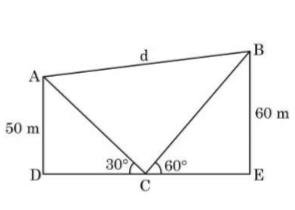
\includegraphics[width=\columnwidth]{cbse/figs/kites.jpeg}
        \caption{}
        \label{fig:kites5}
    \end{figure}
\begin{enumerate}
\item The length of string used (take them straight) for kites $A$ and $B$ as shown in the figure.
\item The distance $d$ between these two kites.
\end{enumerate}
\hfill\brak{10, 2022}
\item In  \figref{fig:as.jpeg}, a tower stands vertically on the ground. From a point on the ground, which is $80m$ away from the foot of the tower, the angle of elevation of the tower is found to be $30\degree$. Find the height of the tower.
    \begin{figure}[H]
        \centering
        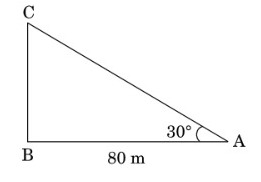
\includegraphics[width=\columnwidth]{cbse/figs/as.jpeg}
        \caption{}
        \label{fig:as.jpeg}
    \end{figure}
    \hfill\brak{10, 2022}
\item The angles of depression of the top and bottom of a tower as seen from the top of a $60\sqrt{3}m$ high cliff are $45\degree$ and $60\degree$ respectively. Find the height of the tower. (Use $\sqrt{3}=1.73$)
    \hfill\brak{10, 2022}\item The angle of elevation of the top of a building from the foot of the tower is $30\degree$ and the angle of elevation of the top of the tower from the foot of the building is $60\degree$. If the tower is $50$ meters high, then find the height of the building.
    \hfill\brak{10, 2022}\item From a point on a bridge across a river, the angles of depression of the banks on opposite sides of the river are $30\degree$ and $60\degree$ respectively. If the bridge is at a height of $3$ meters from the banks, then find the width of the river. 
    \hfill\brak{10, 2022}\item In \figref{fig:ak}, Gadisar Lake is located in the Jaisalmer district of Rajasthan. It was built by the King of Jaisalmer and rebuilt by Gadsi Singh in the $14$th century. The lake has many Chhatris. One of them is shown below:
    \begin{figure}[H]
        \centering
    	 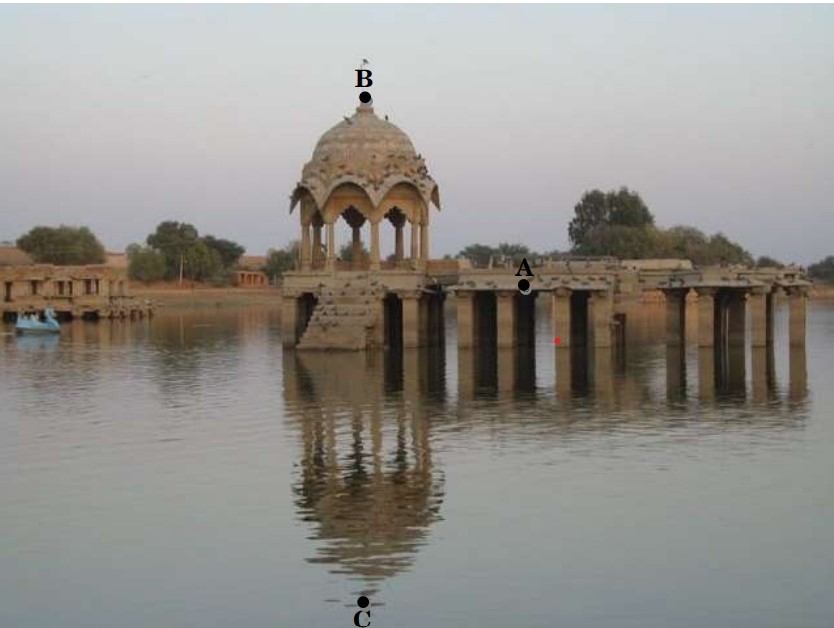
\includegraphics[width=\columnwidth]{cbse/figs/ak.jpeg}
        \caption{}
        \label{fig:ak}
    \end{figure}
    Observe the picture. From a point $Ah$ meters above the water level, the angle of elevation of the top of Chhatri (point $B$) is $45\degree$ and the angle of depression of its reflection in the water (point $C$) is $60\degree$. If the height of Chhatri above water level is (approximately) $10$ meters, then 
\begin{enumerate}
        \item Draw a well-labeled figure based on the above information.
        \item Find the height ($h$) of the point $A$ above water level. (Use $\sqrt{3}=1.73$) 
    \end{enumerate}
%
    \hfill\brak{10, 2022}\item In \figref{fig:su.jpeg}, from a point on a bridge across a river, the angles of depression of the banks on opposite sides of the river are $30\degree$ and $45\degree$. If the bridge is at a height of $8$ meters from the banks, then find the width of the river.
    \begin{figure}[H]
        \centering
        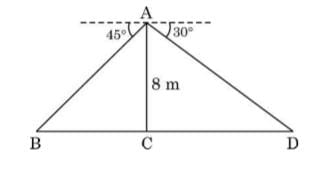
\includegraphics[width=\columnwidth]{cbse/figs/su.jpeg}
        \caption{}
        \label{fig:su.jpeg}
    \end{figure}
    \hfill\brak{10, 2022}
    \item Two boats are sailing in the sea $80$ meters apart from each other towards a cliff $AB$. The angles of depression of the boats from the top of the cliff are $30\degree$ and $45\degree$ respectively, as shown in \figref{fig:boat.jpeg}
%
    \begin{figure}[H]
        \centering
        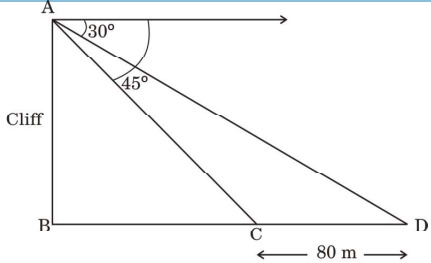
\includegraphics[width=\columnwidth]{cbse/figs/boat.edit.jpeg}
        \caption{}
        \label{fig:boat.jpeg}
    \end{figure}
    Find the height of the cliff.
    \hfill\brak{10, 2022}\item The angle of elevation of the top $Q$ of a vertical tower $PQ$ from a point $X$ on the ground is $60\degree$. From a point $Y$, $40$ meters vertically above $X$, the angle of elevation of the top $Q$ of tower $PQ$ is $45\degree$. Find the height of the tower $PQ$ and the distance $PX$. (Use $\sqrt{3} = 1.73$)
    \hfill\brak{10, 2022}\item An Aeroplane at an altitude of $200$ meters observes the angles of depression of opposite points on the two banks of a river to be $45\degree$ and $60\degree$. Find the width of the river. (Use $\sqrt{3} = 1.732$)
%
    \hfill\brak{10, 2022}\item From the top of an $8$ meter high building, the angle of elevation of the top of a cable tower is $60\degree$ and the angle of depression of its foot is $45\degree$. Determine the height of the tower. (Take $\sqrt{3} = 1.732$).
%
    \hfill\brak{10, 2022}\item As observed from the top of a lighthouse $60$ meters high from the sea level, the angles of depression of two ships are $45\degree$ and $60\degree$. If one ship is exactly behind the other on the same side of the lighthouse, then find the distance between the two ships. (Use $\sqrt{3} = 1.732$)
%
    \hfill\brak{10, 2022}\item At a point on the level ground, the angle of elevation of the top of a vertical tower is found to be $\alpha$, such that $\tan\alpha = \frac{5}{12}$. On walking $192$ meters towards the tower, the angle of elevation $\beta$ is such that $\tan\beta = \frac{3}{4}$. Find the height of the tower.
%
    \hfill\brak{10, 2022}
\item A man on the top of a vertical tower observes a car moving at a uniform speed coming directly towards it. If it takes $18$ minutes for the angle of depression to change from $30\degree$ to $60\degree$, how soon after this will the car reach the tower ?
%
		\hfill\brak{10, 2021}\item A girl on a ship standing on a wooden platform, which is $50m$ above water level, observes the angle of elevation of a top of a hill as $30\degree$ and the angle of depression of the base of the hill as $60\degree$. Calculate the distance of the hill from the platform and the height of the hill.
\hfill\brak{10, 2021}
%
\item The length of the shadow of a tower on the plane ground is $\sqrt{3}$ times the height of the tower. Find the angle of elevation of the sun.
%
\hfill\brak{10,  2023}\item  The angle of elevation of the top of a tower from a point on the ground which is $30m$ away from the foot of the tower, is $30\degree$ . Find the height of the tower. 
%
\hfill\brak{10,  2023}\item  As observed from the top of a $75m$ high lighthouse from the sea-level, the angles of depression of two ships are $30\degree$ and $60\degree$. If one ship is exactly behind the other on the same side of the lighthouse, find the distance between two ships. Use $\brak{\sqrt{3} = 1. 73}$
%
\hfill\brak{10, 2023}\item  From a point on the ground,the angle of elevation of the bottom and top of a transmission tower fixed at the top of $30m$ high building are $30\degree$ and $60\degree$, respectively.Find the height of the transmission tower.Use $\brak{\sqrt{3} = 1.73}$
 \hfill\brak{10, 2023}   
%
\item A straight highway leads to the foot of a tower. A man standing on the top of the $75m$ high tower observes two cars at angles of depression of $30\degree$ and $60\degree$, which are approaching the foot of the tower. If one car is exactly behind the other on the same side of the tower, find the distance between the two cars.
    \hfill\brak{10, 2023}\item From the top of a $7m$ high building, the angle of elevation of the top of a cable tower is $60\degree$ and the angle of depression of its foot is $30\degree$. Determine the height of the tower. (take $\sqrt{3}=1. 73$)
\hfill\brak{10, 2023}\item The angle of elevation of the top of a tower $24m$ high from the foot of another tower in the same plane is ${60}{\degree}$. The angle of elevation of the top of second tower from the foot of the first tower is ${30}{\degree}$. Find the distance between two towers and the height of the other tower. Also, find the length of the wire attached to the tops of both the towers.
\hfill\brak{10, 2023}\item A spherical balloon of radius $r$ subtends an angle of ${60}{\degree}$ at the eye of an observer. If the angle of elevation of its centre is ${45}{\degree}$ from the same point, then prove that height of the centre of the balloon is $\sqrt{2}$ times its radius.
    \hfill\brak{10, 2023}
%
\item A vertical pole is $100$ metres high. Find the angle subtended by the pole at a point on
the ground $100 \sqrt{3}$ meters from the base of the pole.
%
    \hfill\brak{10, 2021}\item The angle of elevation of the top of a tower from a point is found to be $60\degree$. At a point $40m$ above the first point, the angle of elevation of the top of the tower is $45\degree$. Find the height of the tower. 
    \hfill\brak{10, 2021}\item A statue $1.6$m tall stands on the top of a pedestal. From a point on the ground, the angle of elevation of the top of statue is $60\degree$ and from the same point, the angle of elevation of the top of the pedestal is $45\degree$.Find the height of the pedestal.
    \hfill\brak{10, 2021}\item Two poles, $6m$ and $11m$ high, stand vertically on the ground. If the distance between their feet is $12m$ , find the distance between their tops.
%
	\hfill\brak{10, 2021}\item The angle of elevation of the top of a tower from a point on the ground,which is $30m$ away from the foot of the tower is $45\degree$. What is the height of the tower ?
	\hfill\brak{10, 2021}\item Find the sun's altitude if the shadow of a 15$m$ high tower is ${15}\sqrt{3}m$.
	\hfill\brak{10, 2021}\item From a point on the ground, $20m$ away from the foot of vertical tower, the angle of elevation of the top of the tower is $60\degree$. Find the height of the tower.
			\hfill\brak{10, 2021}
\item To explain how trignometry can be used measure the height of an inaccessible object, a teacher gave the following example to students :
%
		A TV tower stands vertically on the bank of a canal.  From a point on the other bank direct opposite the tower, the angle of the elevation of the top of the tower is $60\degree$. From another point 20$m$ away from this point to the foot of the tower, the angle of elevation of the top of the tower is $30\degree$ (as shown in 
			\figref{fig:traingle}
). 
%
		\begin{figure}[H]
			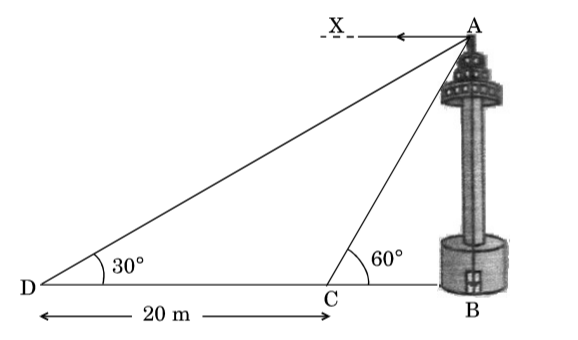
\includegraphics[width=0.75\columnwidth]{cbse/figs/Problem.png}
			\caption{}
			\label{fig:traingle}
		\end{figure}
		Based on the above, answer the following questions 
\begin{enumerate}
			\item The width of the canal is
				\begin{multicols}{4}
\begin{enumerate}
					\item ${10}\sqrt{3} m$
					\item ${20}\sqrt{3} m$
					\item $10 m$
					\item $20 m$
				\end{enumerate}
\end{multicols}
			\item Height of the tower is
				\begin{multicols}{4}
\begin{enumerate}
					\item ${10}\sqrt{3} m$
					\item $10 m$
					\item ${20}\sqrt{3} m$
					\item $20 m$
				\end{enumerate}
\end{multicols}
			\item Distance of the foot of the tower from the point $D$ is
				\begin{multicols}{4}
\begin{enumerate}
					\item $20 m$
					\item $30 m$
					\item $10 m$
					\item ${20}\sqrt{3} m$
				\end{enumerate}
\end{multicols}
\end{enumerate}
\hfill\brak{10, 2021}
\item In \figref{fig:Fig-4.png}, the angle of elevation of the top of a tower from a point $C$ on the ground, which is $30m$ away from the foot of the tower, is $30\degree$. Find the height of the tower.      
\begin{figure}[H]
\centering
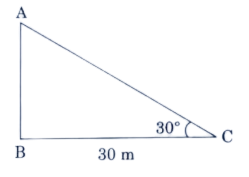
\includegraphics[width=0.75\columnwidth]{cbse/figs/Fig-4.png}
\caption{}      
\label{fig:Fig-4.png}
\end{figure}
\hfill\brak{10, 2020}\item A statue $1.6m$ tall, stands on the top of a pedestal. From a point on the ground, the angle of elevation of the top of the statue is $60\degree$ and from the same point the angle of elevation of the top of the pedestal is $45\degree$. Find the height of the pedestal.(Use $\sqrt{3}=1.73$)
\hfill\brak{10, 2020}
\item A moving boat is observed from the top of a $150m$ high cliff moving away from the cliff. The angle of depression of the boat changes from $60\degree$ to $45\degree$ in $2$ minutes. Find the speed of the boat in $m/min$.
%
\hfill\brak{10, 2019}\item There are two poles, one each on either bank of a river just opposite to each other. One pole is $60m$ high. From the top of this pole, the angle of depression of the top and foot of the other pole are $30\degree$ and $60\degree$respectively. Find the width of the river and height of the other pole.
%
\hfill\brak{10, 2019}\item Two poles of equal heights are standing opposite to each other on either side of the road which is $80 m$ wide. From a point $P$ between them on the road, the angle of elevation of the top of a pole is $60\degree$ and the angle of depression from the top of the other pole of point $P$ is $30\degree$. Find the heights of the poles and the distance of the point $P$ from the poles.
%
\hfill\brak{10, 2019}\item Amit, standing on a horizontal plane, finds a bird flying at a distance of $200 m$ from him at an elevation of $30\degree$. Deepak standing on the roof of a $50 m$ high building, finds the angle of elevation of the same bird to be $45\degree$. Amit and Deepak are on opposite sides of the bird. Find the distance of the bird from Deepak.
%
\hfill\brak{10, 2019}\item From a point $P$ on the ground, the angle of elevation of the top of a tower is $30\degree$ and that of the top of the flag-staff fixed on the top of the tower is $\sqrt{5}$. If the length of the flag-staff is $5 m$, find the height of the tower. (Use $\sqrt{3}= 1.732$).
%
%
\hfill\brak{10, 2019}\item The shadow of a tower standing on a level ground is found to be $40 m$ longer when the Sun's altitude is $30\degree$ than when it was $60\degree$. Find the height of the tower. Given $(\sqrt{3} = 1.732)$
%
\hfill\brak{10, 2019}\item A man in a boat rowing away from a light house $100m$  high takes $2$ minutes to change the angle of elevation of the top of the light house from $60\degree$ to $30\degree$. Find the speed of the boat in metres per minute. [Use $\sqrt{3}=1.732$]
\hfill\brak{10, 2019}\item Two poles of equal heights are standing opposite each other on either side of the road, which is $80 m$  wide. From a point between them on the road, the angles of elevation of the top of the poles are $60\degree$ to $30\degree$ respectively. Find the height of the poles and the distances of the point from the poles.
\hfill\brak{10, 2019}
		\item As observed from the top of a $100 m$ high light house from the sea level, the angles of depression of two ships are $30\degree$ and $45\degree$. If one ship is exactly behind the other on the same side of the light house, find the distance between the two ships. {Use} ($\sqrt3 = 1.732$)
\hfill\brak{10, 2018}
\item A statue, $1.46m$ tall, stands on a pedestal. From a point on the ground the angle of elevation of the top of the statue is $60\degree{}$ and from the same point angle of elevation of the top of the pedestal is $45\degree{}$. Find the height of the pedestal. Use $\brak{\sqrt{3}=1.73}$
\hfill\brak{10, 2018}
\item A ladder, leaning against a wall, makes an angle of $60 \degree$ with the horizontal. If the foot of the ladder is $2. 5m$ away from the wall, find the length of the ladder. 
\hfill\brak{10, 2016}\item  A man standing on the deck of a ship, which is $10m$ above water level, observes the angle of elevation of the top of a hill as $ 60\degree $ and the angle of depression of the base of hill as $ 30 \degree $. Find the distance of the hill from the ship and the height of the hill.
\hfill\brak{10, 2016}\item The angle of elevation of the top $Q$ of a vertical tower $PQ$ from a point $X$ on the ground is $ 60\degree $. From a point $Y$, $40m$ vertically above $X$, the angle of elevation of the top $Q$ of tower is $ 45 \degree $. Find the height of the tower $PQ$ and the distance $PX$. $\brak{\text{Use }\sqrt{3} = 1.73}$
\hfill\brak{10, 2016}
\item A boy standing on a horizontal plane finds a bird flying at a distance of $100 m$ from him at an elevation of $30\degree$. A girl standing on the roof of a $20 m$ high building, finds the elevation of the same bird to be $45\degree$. The boy and the girl are on the opposite sides of the bird. Find the distance of the bird from the girl. (Given ${\sqrt 2}= 1.414$)
%
\hfill\brak{10, 2019}\item The angle of elevation of an aeroplane from a point $A$ on the ground is $60\degree$. After a flight of $30$ seconds, the angle of elevation changes to $30\degree$. If the plane is flying at a constant height of $3600\sqrt 3 $ metres, find the speed of the aeroplane.
%
\hfill\brak{10, 2019}
\item If a tower $30m$ high, casts a shadow $10\sqrt{3}m$ long on a ground, then what is the angle of elevation of the sun ?
\hfill\brak{10, 2017}\item A man observes a car from the top of a tower, which is  moving towards the tower with a uniform speed. If the angle of depression of the car changes from $30\degree$ to $45\degree$ in $12$ minutes, find the time taken by the car now to reach the tower.
\hfill\brak{10, 2017}\item An aeroplane is flying at a height of $300 m$ above the ground. Flying at this height, the angles of depression from the aeroplane of two points on both banks of a river in opposite directions are $45\degree$ and $60\degree$ respectively. Find the width of the river. 
\hfill Use $\sbrak{\sqrt 3 = 1.732}$
\hfill\brak{10, 2017}\item On a straight line passing through the foot of a tower, two points $C$$D$ are at distances of $4$ m
and $16m$ from the foot respectively. If the angles of elevation from$C$$D$ of the top tower are complementary, then find the height of the tower.  
\hfill\brak{10, 2017}\item From the top of a tower, $100m$ high, a man observes two cars on the opposite sides of the tower and in same straight line with its base, with angles of depression $30\degree$ and $45\degree$. Find the distance between the cars.
Take $\sbrak{\sqrt{3} = 1.732}$
\hfill\brak{10, 2017}
\item At a point $A$, $20$ metres above the level of water in a lake, the angle of elevation of a cloud is $30 \degree$. The angle of depression of the reflection of the cloud in the lake, at $A$ is $60\degree $. Find the distance of the cloud from $A$.
\hfill\brak{10,  2015}\item In Figure \ref{Figure 1},  a tower $AB$ is $20m$ high and $BC$,  its shadow on the ground, is $20\sqrt{3}m$ long. Find the sun's altitude.
\begin{figure}[H]
	\centering
    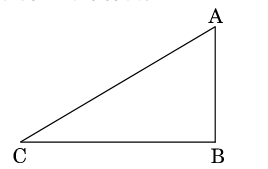
\includegraphics[width=\columnwidth]{cbse/figs/cbse_30_3_1.png}
	\caption{}
	\label{Figure 1}
\end{figure}
\hfill\brak{10, 2015}\item The angle of elevation of an aeroplane from a point $A$ on the ground is $60 \degree  $. After a flight of $15$ seconds, the angle of elevation changes to $  30 \degree.$ If the aeroplane is flying at a constant height of $1500\sqrt{3}$ m, find the speed of the plane in $km/hr$.
\hfill\brak{10, 2015}
\item A kite is flying at a height of $30 { m}$ from the ground. The length of string from the kite to the ground is $60 { m}$. Assuming that there is no slack in the string, the angle of elevation of the kite at the ground is \rule{1cm}{0.1pt}. 
\hfill\brak{10, 2012}\item From a point on the ground, which is $15{ m}$ away from the foot of a vertical tower, the angle of elevation of the top of the tower, is found to be $60\degree$. The height of the tower in (in metres) is 
\rule{1cm}{0.1pt}.
\hfill\brak{10, 2012}\item The length of shadow of a tower on the plane ground is $\sqrt 3 m$ times the height of the tower. The angle of elevation of sun is  \rule{1cm}{0.1pt}.
\hfill\brak{10, 2012}\item The angles of depression of the top and bottom of a tower as seen from the top of a $60\sqrt 3 { m}$ high cliff are $45\degree$ and $60\degree$ respectively. Find the height of the tower. 
%Trigonometry
\hfill\brak{10, 2012}\item In a flight of $2800 { km}$, an aircraft was slowed down due to bad weather. Its average speed is reduced by $100 { km/h}$ and time is increased by $30$ minutes. Find the original duration of flight. 
%Trigonometry
\hfill\brak{10, 2012}\item The angles of elevation and depression of the top and bottom of a light-house from the top of a $60 { m}$ high building are $30\degree$ and $60\degree$ respectively. Find 
\begin{enumerate}
\item the difference between the heights of the light-house and the building. 
\item the distance between light-house and building. 
\end{enumerate}
\hfill\brak{10, 2012}\item The angles of depression of two ships from the top of a light house and on the same side of it are found to be $45\degree$ and $30\degree$. if the ships are $200 { km}$ apart, find the height of the light house. 
\hfill\brak{10, 2012}\item The angle of elevation of the top of a hill at the foot of a tower is $60\degree$ and the angle of depression from the top of the tower of the foot of the hill is $30\degree$. If the tower is $50{ m}$ high, find the height of the hill. 
\hfill\brak{10, 2012}\item From the top of a tower $50{ m}$ high, the angle of depression of the top of a pole is $45\degree$ and from the foot of the pole, the angle of elevation of the top of the tower is $60\degree$. find the height of the pole if the pole and tower stand on the same plane. 
\hfill\brak{10, 2012}\item The angle of depression from the top of a tower of a point $A$ on the ground is $30\degree$. On moving a distance of $20{ m}$ from the point $A$ towards the foot of the tower to a point $B$ the angle of elevation of the top of the tower from point $B$ is $60\degree$. Find the height of the tower and its distance from point $A$.
\hfill\brak{10, 2012}
\item A tower stands vertically on the ground. From a point on the ground which is $25m$ away from the foot of the tower, the angle of elevation of the top of the tower is found to be $45\degree$. Then the height $\brak{in\,meters}$ of the tower is
%
%
%
\hfill\brak{10, 2011}\item The angle of elevation of the top of a vertical tower from a point on the ground is $60\degree$. From another point $10m$ vertically above the first, its angle of elevation is $30\degree$. Find the height of the tower.
%
%
\hfill\brak{10, 2011}\item From the top of a vertical tower, the angles of depression of two cars, in the same straight line with the base of the tower, at an instant are found to be $45\degree$ and $60\degree$. If the cars are $100m$ apart and are on the same side of the tower, find the height of the tower. 
%
[Use $\sqrt{3} = 1.73$]
\hfill\brak{10, 2011}
    \item The angle of elevation of the top of a tower from a point on the ground, which is 30$m$ away from the foot of the tower is 45\degree. The height of the tower (in metres) is
    \hfill\brak{10, 2011}\item From the top of a tower $100m$ high, a man observes two cars on the opposite sides of the tower with angles of depression $30\degree$ and $45\degree$ respectively. Find the distance between the cars. [Use $\sqrt{3}=1.73$].
    \hfill\brak{10, 2011}\item Two poles of equal heights are standing opposite to each other on either side of the road, which is $100m$ wide. From a point between them on the road, the angles of elevation of the top of the poles are $60\degree$ and $30\degree$, respectively. Find the height of the poles.
\hfill\brak{10, 2011}
%
\item A man standing on the deck of a ship, which is 10$m$ above the water level, observes the
angle of elevation of the top of a hill as 60\degree and the angle of depression of the base of the hill as
30\degree. Calculate the distance of the hill from the ship and the height of the hill.
%
\hfill\brak{10, 2006}\item From a window $x$ meters high above the ground in a street, the angles of elevation and depression of the top and foot of the other house on the opposite side of the street are $\alpha$ and $\beta$ respectively. Show that the height of the opposite house is $x(1 + \tan \alpha \cot \beta)$ meters.
%
\hfill\brak{10, 2006}
%
\item A pole $6m$ high is fixed on the top of a tower. The angle of elevation of the top of the pole observe
d from a point $P$ on the ground is $60\degree$ and the angle of depression of the point $P$ from the top of
 the tower is $45\degree$. Find the height of the tower and the distance of point $P$ from the foot of the tower
\hfill\brak{10, 2024}
%
\item The length of the shadow of a tower on the plane ground is $ \sqrt3 $ times the height of the tower. Find the angle of elevation of the sun.
%
\hfill\brak{10,  2023}\item The angle of elevation of the top of a tower from a point on the ground which is $30 {m}$ away from the foot of the tower, is $30\degree$. Find the height of the tower. 
\hfill\brak{10, 2023}
%
\item As observed from the top of a $75{m}$ high lighthouse from the sea-level, the angles of depression of two ships are $30\degree$ and $60\degree$. If one ship is exactly behind the other on the same side of the lighthouse, find the distance between the two ships.
	Use $\brak{\sqrt{3} = 1.73}$
%
\hfill\brak{10, 2023}\item From a point on the ground, the angle of elevation of the bottom and top of a transmission tower fixed at the top of $30 {m}$ high building are $30\degree$ and $60\degree$, respectively. Find the height of the transmission tower. Use $\brak{\sqrt{3} = 1.73}$.
	\hfill\brak{10, 2023}\item If a pole  $6m$ high casts a shadow $2 \times \sqrt{3}m$ long on the ground, then sun's elevation is
	\begin{multicols}{4}
\begin{enumerate}
\item $60\degree$
\item $45\degree$
\item $30\degree$
\item $90\degree$
	\end{enumerate}
\end{multicols}
 \hfill\brak{10, 2023}
%
\item
	A straight highway leads to the foot of a tower. A man standing on the top of the $75 {m}$ high tower observes two cars at angles of depression of $30\degree$ and $60\degree$, which are approaching the foot of the tower. If one car is exactky behind the other on the same side of the tower, find the distance between the two cars. Use \brak{\sqrt{3}=1.73}.
\hfill\brak{10, 2023}\item
	From the top of a $7 {m}$ building, the angle of elevation of the top a cable tower is 60\degree and the angle of depression of its foot is 30\degree. Determine the height of the tower.
%
\hfill\brak{10, 2023}
%
\end{enumerate}

\subsection{JEE}
\begin{enumerate}[label=\thesubsection.\arabic*,ref=\thesubsection.\theenumi]
\item A person standing on the bank of a river observes that the angle of elevation of the top of a tree on the opposite bank of the river is $60\degree$ and when he retires $40$ meters away from the tree, the angle of elevation becomes $30\degree$. The breadth of the river is 
%

\hfill\brak{2004}
\begin{multicols}{4}
\begin{enumerate}
        \item $60m$                    
        \item $30m$ 
        \item $40m$ 
        \item $20m$
\end{enumerate}
\end{multicols} 
%
\item A tower stand at the centre of a circular park. ${A}$ and ${B}$ are two points on the boundary of the park such that AB $\brak{=a}$ subtends an angle of $60\degree$ at the foot of the tower, and the angle of elevation of the top of the tower from ${A}$ or ${B}$ is $30\degree.$ The height of the tower is \hfill\brak{2007}
\begin{multicols}{4}
\begin{enumerate}
        \item $\frac{a}{\sqrt{3}}$                    
        \item $a\sqrt{3}$ 
        \item $\frac{2a}{\sqrt{3}}$ 
        \item $2a\sqrt{3}$
\end{enumerate}
\end{multicols} 
%
\item AB is a vertical pole with ${B}$ at the ground level and ${A}$ at the top. A man finds that the angle of elevation the the point ${A}$ from a certain point ${C}$ on the ground is $60\degree.$ He moves away from the pole along the line BC to a point ${D}$ such that $\text{CD}=7m.$ From ${D}$ the angle of elevation of point ${A}$ is $45\degree.$ Then the height of the pole is  
%
\hfill\brak{2008}
\begin{multicols}{4}
\begin{enumerate}
	\item $\frac{7\sqrt{3}}{2\brak{\sqrt{3}-1}}m$
        \item $\frac{7\sqrt{3}}{2}\brak{\sqrt{3}+1}m$ 
        \item $\frac{7\sqrt{3}}{2}\brak{\sqrt{3}-1}m$ 
	\item $\frac{7\sqrt{3}}{2\brak{\sqrt{3}+1}}m$
\end{enumerate}
\end{multicols} 
\item A bird is sitting on the top of a vertical pole $20m$ high and its elevation from a point ${O}$ on the  ground is $45\degree.$ It flies off horizontally straight away from the point ${O}$. After one second, the elevation of the bird from ${O}$ is reduced to $30\degree.$ Then the speed in \brak{m/s} of the bird is \hfill\brak{2014}
\begin{multicols}{4}
\begin{enumerate}
        \item $20\sqrt{2}$                    
        \item $20\brak{\sqrt{3}-1}$ 
        \item $40\brak{\sqrt{2}-1}$ 
        \item $40\brak{\sqrt{3}-\sqrt{2}}$
\end{enumerate}
\end{multicols} 
%
\item If the angle of elevation of the top of a tower from three colinear points ${A},{B}\text{ and }{C}$ on a line leading to foot of the tower, are $30\degree,45\degree$ and  $60\degree$ respectively, then the ratio, $\text{AB}:\text{BC},$ is: 
\hfill\brak{2015}
\begin{multicols}{4}
\begin{enumerate}
        \item $1:\sqrt{3}$                    
        \item $2:3$ 
        \item $\sqrt{3}:1$ 
        \item $\sqrt{3}:\sqrt{2}$
\end{enumerate}
\end{multicols} 
%
\item Let a vertical tower AB have its end ${A}$ on the level ground. Let ${C}$ be the  mid-point of AB and ${P}$ be a point on the ground such that $\text{AP}=2\text{AB}.$ If $\angle{BPC}=\beta,$ then $\tan \beta$ is equal to: \hfill\brak{ 2017}
\begin{multicols}{4}
\begin{enumerate}
        \item $\frac{4}{9}$                    
        \item $\frac{6}{7}$ 
        \item $\frac{1}{4}$ 
        \item $\frac{2}{9}$
\end{enumerate}
\end{multicols} 
%
\item $\triangle{PQR}$ is a triangular park with $\text{PQ}=\text{PR}=200m$. A T.V. tower stands at the mid-point of QR. If the angles of the elevation of the top of the tower at ${P,Q \text{ and } R}$ are respectively $45\degree , 30\degree \text{ and } 30\degree,$ then the height of the tower in $m$ is \hfill\brak{ 2018}
\begin{multicols}{4}
\begin{enumerate}
        \item $50$                    
        \item $100\sqrt{3}$ 
        \item $50\sqrt{2}$ 
        \item $100$
\end{enumerate}
\end{multicols} 
    \item From the top of a light-house $60 $ meter high with its base at the sea level the angle of depression of a boat is  $15\degree$. The distance of the boat from the foot of the light house.
		 \hfill (1983)
	    \begin{multicols}{2}    
\begin{enumerate}
    \item $\brak{\frac{\sqrt{3}-1}{\sqrt{3}+1}}60 $ metres 
    \item $\brak{\frac{\sqrt{3}+1}{\sqrt{3}-1}}60 $ metres 
    \item $\brak{\frac{\sqrt{3}+1}{\sqrt{3}-1}}^2 60 $ metres 
    \item none of these 
\end{enumerate}
	    \end{multicols}
\item A pole stands vertically inside a triangular park $\triangle ABC$. If the angle of elevation of the top of the pole from each corner of the park is same, then in $\triangle ABC$ the foot of the pole is at the
\hfill (2000)
	    \begin{multicols}{2}    
\begin{enumerate}
\item centroid
\item circumcentre
\item incentre
\item orthocentre
\end{enumerate}
	    \end{multicols}
%
\item A man from the top of a $100$ metres high tower sees a car moving towards the tower at an angle of depression of $30\degree$. After some time, the angle of depression becomes $60\degree$. The distance (in metres) travelled by the car during this time is
\hfill (2001)
	    \begin{multicols}{4}    
\begin{enumerate}
\item $100\sqrt{3}$
\item $\frac{200\sqrt{3}}{3}$
\item $\frac{100\sqrt{3}}{3}$
\item $200\sqrt{3}$
\end{enumerate}
	    \end{multicols}
     	\item A baloon is observed simultaneously from three points ${A},{B} \text{ and } {C}$ on a straight road directly beneath it. The angular elevation at ${B}$ is twice that at ${A}$ and angular elevation at ${C}$ is thrice that of ${A}$. If the distance between ${A}$ and ${B}$ is $a$ and the distance between ${B}$ and ${C}$ is $b$, find height of baloon in terms of $a \text{ and } b$.
     \hfill {(1980)}
\item $PQ$ is a vertical tower. $P$ is the foot and $Q$ is the top of the tower. $A$, $B$, $C$ are three points in the horizontal plane through P. The angles of elevation of $Q$ from $A$, $B$, $C$ are equal, and each is equal to $\theta$. The sides of the triangle $ABC$ are $a$, $b$, $c$; and the area of the triangle $ABC$ is $\Delta$. Show that the height of the tower is $\frac{abc\tan{\theta}}{4\Delta}$.
\item $AB$ is a vertical pole. The end $A$ is on the level ground. $C$ is the middle point of $AB$. $P$ is a point on the level ground. The portion $CB$ subtends an angle $\beta$ at $P$. If $AP=nAB$ then show that $\tan{\beta}=\frac{n}{2n^2+1}$.
%
\hfill{\brak{1980}}
\item A vertical pole stands at a point $Q$ on a horizontal ground. $A$ and $B$ are points on the ground, $d$ meters apart. The pole subtends angles $\alpha$ and $\beta$ at $A$ and $B$ respectively. $AB$ subtends an angle $\gamma$ at $Q$. Find the height of the pole. 
%
\hfill{\brak{1982}}
%
\item Four ships $A$, $B$, $C$ and $D$ are at sea in the following relative positions: $B$ is on the straight line segment $AC$, $B$ is due North of $D$ and $D$ is due west of $C$. The distance between $B$ and $D$ is $2 km$. $\angle{BDA}=40\degree$, $\angle{BCD}=25\degree$. What is the distance between $A$ and $D$? $\sbrak{\text{Take} \sin{25\degree}=0.423}$
%
\hfill{\brak{1983}}
%
\item A ladder rests against a wall at an angle $\alpha$ to the horizontal. Its foot is pulled away from the wall through a distance $a$, so that it slides a distance $b$ down the wall making an angle $\beta$ with the horizontal. Show that $a=b\tan{\frac{1}{2}\brak{\alpha+\beta}}$.
%
\hfill{\brak{1985}}
\item A sign-post in the form of an isosceles triangle $ABC$ is mounted on a pole of height $h$ fixed to the ground. The base $BC$ of the triangle is parallel to the ground. A man standing on the ground at a distance $d$ from the sign-post finds that the top vertex $A$ of the triangle subtends an angle $\beta$ and either of the other two vertices subtends the same angle $\alpha$ at his feet. Find the area of the triangle. 
%
\hfill{\brak{1988}}
%
\item $ABC$ is a triangular park with $AB=AC=100$m. A television tower stands at the midpoint of $BC$. The angles of elevation of the top of the tower at $A$, $B$, $C$ are $45\degree$, $60\degree$, $60\degree$, respectively. Find the height of the tower. 
%
\hfill{\brak{1989}}
%
\item A vertical tower $PQ$ stands at a point $P$. Points $A$ and $B$ are located to the South and East of $P$ respectively. $M$ is the mid point of $AB$. $PAM$ is an equilateral triangle; and $N$ is the foot of the perpendicular from $P$ on $AB$. Let $AN=20$ metres and the angle of elevation of the top of the tower at $N$ is $\tan^{-1}{2}$. Determine the height of the tower and the angles of elevation of the top of the tower at $A$ and $B$.
%
\hfill{\brak{1990}}
%
\item A man notices two objects in a straight line due west. After walking a distance $c$ due north he observes that the objects subtend an angle $\alpha$ at his eye; and, after a further distance $2c$ due north, an angle $\beta$. Show that the distance between the objects is $\frac{8c}{3\cot{\beta}-\cot{\alpha}}$; the height of the man is being ignored. 
%
\hfill{\brak{1991}}
\end{enumerate}

%
\section{Triangle}
\subsection{NCERT}
\begin{enumerate}[label=\thesubsection.\arabic*.,ref=\thesubsection.\theenumi]

\item  $D$ is a point on the side $BC$ of a $\triangle ABC$ such that  $\angle  ADC =  \angle  BAC$. Show that 
\begin{align}
	\label{eq:tri-sim}	
	CA^2 = CB.CD
\end{align}
%
	\\
		\solution
	See \figref{fig:tri-sim}.	
\begin{align}
	\frac{x}{\sin\brak{A+C}} &= 
	\frac{b}{\sin A}  
\quad 
		\brak{\triangle ADC},
		\\
	\implies	\frac{x}{\sin B} &= 
	\frac{b}{\sin A}  
	\\
\implies	\frac{x}{b} = 
	\frac{\sin B}{\sin A}  &= 
	\frac{b}{a}  \quad \brak{\text{ sine formula }}
\end{align}
yielding
	\eqref{eq:tri-sim}.	
\begin{figure}[H]
	\begin{center}
			\resizebox{0.6\columnwidth}{!}{\input{figs/tri/tri-sim.tex}}
	\end{center}
	\caption{}
	\label{fig:tri-sim}	
\end{figure}
\item   $D$ is a point on side $BC$ of  $\triangle  ABC$ such that
$\frac{BD}{CD}= \frac{AB}{AC}  $.  Prove that $AD$ is the bisector of  $\angle  BAC$.
\\
\solution 
	See \figref{fig:tri-ang-bis}.	
\begin{align}
	\frac{x}{a-x} &= 
	\frac{c}{b}  \quad \brak{\text{ given }}
	\\
	\frac{c}{\sin\phi} &= 
	\frac{x}{\sin \theta}  \quad \brak{\triangle ABD}
	\\
	\frac{a-x}{\sin\brak{A-\theta}} &= 
	\frac{b}{\sin 180-\phi}  \quad \brak{\triangle ACD}
	\\
	&=\frac{b}{\sin \phi}
\end{align}
using the sine formula.  Multiplying all the above equations yields
\begin{align}
	\sin \brak{A-\theta}
	=\sin \theta \implies \theta = \frac{A}{2}
\end{align}
\begin{figure}[H]
	\begin{center}
			\resizebox{0.6\columnwidth}{!}{\input{figs/tri/tri-ang-bis.tex}}
	\end{center}
	\caption{}
	\label{fig:tri-ang-bis}	
\end{figure}
%
\item  $ABC$ is a triangle in which  $\angle  ABC > 90\degree$ and $AD  \perp  CB$ produced. Prove that
\begin{align}
	\label{eq:tri-obtuse}
 AC^2= AB^2 + BC^2 + 2 BC . BD.
\end{align}
\solution
	See \figref{fig:tri-obtuse}.	
\begin{align}
	\label{eq:tri-obtuse-1}
	\cos B &= \frac{x}{c} \quad \brak{\triangle ADB}
	\\
	b^2 &= a^2 + c^2 -2ac \cos \brak{180-B} \quad \brak{\triangle ABC}
	\\
	&= a^2 + c^2 +2ac \cos B 
	\label{eq:tri-obtuse-2}
\end{align}
using the cosine formula.
Substituting from 
	\eqref{eq:tri-obtuse-1}
	in
	\eqref{eq:tri-obtuse-2}
	yields 
	\eqref{eq:tri-obtuse}.
\begin{figure}[H]
	\begin{center}
			\resizebox{0.6\columnwidth}{!}{\input{figs/tri/tri-obtuse.tex}}
	\end{center}
	\caption{}
	\label{fig:tri-obtuse}	
\end{figure}
\item In a right triangle, prove that the line-segment joining the mid-point of the hypotenuse to the opposite vertex is half the hypotenuse.
	\\
	\solution
	In \figref{fig:tri-hyp}	
\begin{align}
	\label{eq:tri-hyp}	
	\frac{x}{\sin C} &= \frac{b/2}{\sin \theta} \quad \brak{\triangle BDC}
	\\
	\frac{x}{\sin A} &= \frac{b/2}{\sin \brak{90-\theta}} \quad \brak{\triangle BDA}
	\\
\implies	\frac{x}{\cos C} &= \frac{b/2}{\cos \theta} 
	\label{eq:tri-hyp-1}	
\end{align}
From 
	\eqref{eq:tri-hyp}	
	and
	\eqref{eq:tri-hyp-1},
\begin{align}
	\brak{\frac{\sin C}{x}}^2
	+
	\brak{\frac{\cos C}{x}}^2
	&= 
	\brak{\frac{\cos \theta}{\frac{b}{2}}}^2
	+
	\brak{\frac{\sin \theta}{\frac{b}{2}}}^2
	\\
	\implies x &= \frac{b}{2} 
\end{align}
using \eqref{eq:tri_sin_cos_id}.
\begin{figure}[H]
	\begin{center}
			\resizebox{0.6\columnwidth}{!}{\input{figs/tri/tri-hyp.tex}}
	\end{center}
	\caption{}
	\label{fig:tri-hyp}	
\end{figure}
\item $ABCD$ is a trapezium in which $AB  \parallel  DC$ and its diagonals intersect each other at the point $O$. Show
that
\begin{align}
	\label{eq:tri-trap}	
\frac{AO}{ BO}=\frac{CO}{  DO}
\end{align}
\begin{figure}[H]
	\begin{center}
			\resizebox{0.6\columnwidth}{!}{\input{figs/tri/tri-trap.tex}}
	\end{center}
	\caption{}
	\label{fig:tri-trap}	
\end{figure}
\solution 
	In \figref{fig:tri-trap}, $\because AB \parallel CD$	
\begin{align}
	\frac{AO}{\sin \phi} &= \frac{BO}{\sin \theta} \quad \brak{\triangle OAB}
	\\
	\frac{CO}{\sin \phi} &= \frac{DO}{\sin \theta} \quad \brak{\triangle ODC}
\end{align}
yielding
	\eqref{eq:tri-trap}	
	after simplification.
\item $O$ is any point inside a rectangle $ABCD$. Prove that 
\begin{align}
	OB^2+OD^2 = OA^2+OC^2
	\label{eq:tri-rect}	
\end{align}
	\solution
	In 
	\figref{fig:tri-rect},	
from \eqref{ch1_budh_basic}
\begin{align}
	p \cos \theta_1+q \sin \theta_2 = a \quad \brak{\triangle OAB}
	\\
	r \cos \theta_3+s \sin \theta_4 = a \quad \brak{\triangle OAB}
	\\
	p \cos \theta_1+s \sin \theta_4 = b \quad \brak{\triangle OAB}
	\\
	r \cos \theta_3+q \sin \theta_2 = b \quad \brak{\triangle OAB}
\end{align}
Subtracting the first two and second two equations respectively,
\begin{align}
	p \cos \theta_1 
	-s \sin \theta_4  
= r \cos \theta_3-q \sin \theta_2
\\
	p \cos \theta_1+s \sin \theta_4 = 
	r \cos \theta_3+q \sin \theta_2  
\end{align}
Squaring and adding and using 
\eqref{eq:tri_sin_cos_id}
yields
	\eqref{eq:tri-rect}.	
\begin{figure}[H]
	\begin{center}
			\resizebox{0.6\columnwidth}{!}{\input{figs/tri/tri-rect.tex}}
	\end{center}
	\caption{}
	\label{fig:tri-rect}	
\end{figure}
\item  In  $\triangle  ABC, AB = 6\sqrt{3} cm, AC = 12 cm$ and $BC = 6 cm$. Find the angle $B$.
	\\
	\solution Using 
\eqref{eq:tri_cos_form},
\begin{align}
	\cos B &= 
 \frac{c^2+a^2-b^2}{2ca}=0
	\\
	\implies B &= 90\degree
\end{align}
\end{enumerate}

\subsection{CBSE}
\begin{enumerate}
	\item In an equilateral $\triangle ABC, D$ is a point on side $BC$ such that $ BD =\frac{1}{3}BC$. Prove that $9(AD)^2 = 7(AB)^2$.
	\hfill\brak{10, 2018}
\item Prove that the area of an equilateral triangle described on one side of the square is equal to half of the area of the equilateral triangle described on one of its diagonal.
	\hfill\brak{10, 2018}\item If the areas of two similar triangles are equal, prove that they are congruent.
\hfill\brak{10, 2018}
\item In \figref{fig:rightangled4}, $BN$ and $CM$ are medians of a $\triangle ABC$ right-angled at $A$. Prove that \begin{align*}4(BN^2 +CM^2) = 5BC^2\end{align*} 
\begin{figure}[H]
\centering
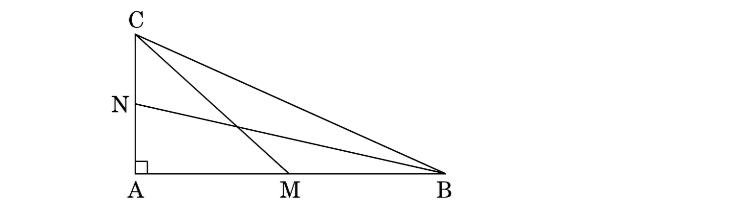
\includegraphics[width=\columnwidth]{cbse/figs/rightangled}
\caption{}
\label{fig:rightangled4}
\end{figure}
%
\hfill\brak{10, 2022}\item If $A$, $B$ and $C$ are interior angles of $ \triangle ABC$, then show that
	\begin{align*}
	    \cos \brak{\frac{B + C}{2}}=\sin \brak{\frac{A}{2}}
	\end{align*}
%      
\hfill\brak{10, 2020} 
\item  In $\triangle ABC$, right-angled at $A$, if $AB=7 cm$ and $AC=24 cm$, then find $\sin B$
and $\tan C$.
%

\hfill\brak{10, 2021}\item Two angles of a triangle are  $\cot^{-1}2$ and $\cot^{-1}3$. The third angle of the
triangle is \rule{1cm}{0.1pt}.
%
\hfill\brak{12, 2021}
%
\item $A$, $B$ and $C$ are interior angles of a triangle $ABC$. Show that
\begin{enumerate}
\item  $\sin$ $ \brak{{\frac {B+C}{2}}} = \cos {\frac {A}{2}}$
\item  If $\angle A = 90 \degree$, then find the value of $\tan \brak{{\frac{B+C}{2}}}$.
\end{enumerate} 
%
\hfill\brak{10, 2019}	\item In $\triangle$ $ABC$, $AB = {4\sqrt{3}}$ cm, $AC = 8 cm$ and $BC = 4 cm$. The angle $B$ is
	\begin{multicols}{4}
				\begin{enumerate}
\item $120\degree$
\item $90\degree$
\item $60\degree$
\item $45\degree$
				\end{enumerate}
\end{multicols}
	\hfill\brak{10, 2021}
%
\end{enumerate}

\subsection{JEE}
 \begin{enumerate}[label=\thesubsection.\arabic*,ref=\thesubsection.\theenumi]
    \item In a $\triangle ABC$, $\angle A=90\degree$ and $AD$ is an altitude. Complete the relation
    $$\frac{BD}{BA} = \frac{AB}{(\dots)}.$$
    \hfill (1980)
    
    \item $ABC$ is a triangle, $P$ is a point on $AB$, and $Q$ is point on $AC$ such that $\angle AQP = \angle ABC$. Complete the relation
	    $$\frac{ar\brak{\triangle APQ}}{ar\brak{\triangle ABC}} =\frac{(\dots)}{AC^2}$$
    \hfill (1980)
    
    \item $ABC$ is a triangle with $\angle B $ greater than $\angle C$.
    $D$ and $E$ are the points on $BC$ such that $AD$ is perpendicular to $BC$ and $AE$ is the bisector of angle $A$. Complete the relation
    $$\angle DAE = \frac{1}{2} [( ) - \angle C].$$
    \hfill (1980)
    \item The set of all real numbers $a$ such that $a^2 + 2a, 2a + 3$ and $a^2 + 3a + 8$ are the sides of a triangle is \rule{1cm}{0.1pt}.
    \hfill (1985)
    \item In   $\triangle ABC$, if $\cot A, \cot B, \cot C$ are in A.P., then $a^2,b^2,c^2$ are in \rule{1cm}{0.1pt} progression 

	    \hfill (1985)
    \item If in the $\triangle ABC$, 
	    $$\frac{2\cos A}{a} + \frac{2\cos B}{b} + \frac{2\cos C}{c} = \frac{a}{bc} +  \frac{b}{ac},$$ 
		then the value of the angle $A$ is \rule{1cm}{0.1pt} degrees. \hfill (1993)
    \item In the $\triangle ABC$, $AD$ is the altitude from $A$. Given $b>c$, $\angle C=23 \degree$ and $AD = \frac{abc}{b^2 - c^2}$ then $\angle B =  \rule{1cm}{0.1pt}$.\hfill (1994)
%
\item In a $\triangle{ABC}$, medians $AD$ and $BE$ are drawn. If $AD=4,\angle{DAB}=\frac{\pi}{6}$  and $\angle{ABE}=\frac{\pi}{3}$, then the area of the $\triangle{ABC}$ is \hfill\brak{2003}
\begin{multicols}{4}
\begin{enumerate}
        \item $\frac{64}{3}$                    
        \item $\frac{8}{3}$ 
        \item $\frac{16}{3}$ 
        \item $\frac{32}{3\sqrt{3}}$
\end{enumerate}
\end{multicols} 
%
\item If in $\triangle{ABC},a\cos^2\brak{\frac{{C}}{2}} + c\cos^2\brak{\frac{{A}}{2}} = \frac{3b}{2},$ then the sides $a,b\text{ and }c$ \hfill\brak{2003}
\begin{multicols}{4}
\begin{enumerate}
        \item satisfy $a+b=c$                    
        \item are in A.P. 
        \item are in G.P. 
        \item are in H.P.
\end{enumerate}
\end{multicols} 
%
\item The sides of a triangle are $\sin\alpha,\cos\alpha$ and $ \sqrt{1+\sin\alpha\cos\alpha}$ for some $0<\alpha<\frac{\pi}{2}.$ Then the greatest angle of the triangle is \hfill\brak{2004}
\begin{multicols}{4}
\begin{enumerate}
        \item $150\degree$                    
        \item $90\degree$ 
        \item $120\degree$
        \item $60\degree$
\end{enumerate}
\end{multicols} 
%
\item In a $\triangle{ABC}$, let $\angle{C}=\frac{\pi}{2}.$ If $r$ is the inradius and $R$ is the circumradius of the $ \triangle{ABC},$ then $2\brak{R+r}$ equals \hfill\brak{2005}
\begin{multicols}{4}
\begin{enumerate}
        \item $b+c$                    
        \item $a+b$ 
        \item $a+b+c$ 
        \item $c+a$
\end{enumerate}
\end{multicols} 
%
\item If in a $\triangle ABC,$ the altitudes from the vertices ${A,B,C}$ on opposite sides are in H.P., then $\sin {A},\sin {B},\sin {C}$ are in \hfill\brak{2005}
\begin{multicols}{4}
\begin{enumerate}
        \item $G.P.$                    
        \item $A.P.$ 
        \item $A.P.-G.P.$ 
        \item $H.P.$
\end{enumerate}
\end{multicols} 
%
    \item There exists a $\triangle ABC$ satisfying the conditions
    \hfill{(1986)}
\begin{multicols}{2}
    \begin{enumerate}
    	\item $b\sin{A} = a, A <\pi/2$
    	\item $b\sin{A} > a, A >\pi/2$
    	\item $b\sin{A} > a, A <\pi/2$
    	\item $b\sin{A} < a, A <\pi/2$, $b > a$
    	\item $b\sin{A} < a, A >\pi/2$, $b = a$
    \end{enumerate}
\end{multicols} 
    \item In a triangle, the lengths of two larger sides are $10$ and $9$ respectively. If the angles are in AP, Then length of third side is
    \hfill{(1987)}
    \begin{multicols}{2}
    	\begin{enumerate}
    		\item $5-\sqrt{6}$ 
    		\item $3\sqrt{3}$
    		\item $3$
    		\item $5+\sqrt{6}$ 
    		\item none
    	\end{enumerate}
    \end{multicols}
    \item If in a $\triangle PQR$, $\sin{P}, \sin{Q}, \sin{R}$ are in AP, then
    \hfill{(1998)}
    \begin{multicols}{2}
    \begin{enumerate}
    	\item The altitudes are in AP
    	\item The altitudes are in HP
    	\item The medians are in GP
    	\item The medians are in AP
    \end{enumerate}
    \end{multicols}
    \item In $\triangle ABC$, internal angle bisector of $\angle A$ meets side $BC$ in ${D}$. $DE \perp AD$ meets $AC$ in ${E}$ and $AB$ in ${F}$. Then
    \hfill{(2006)}
    \begin{multicols}{2}
    \begin{enumerate}
    	\item $AE$ is HM of $b \text{ and } c$
    	\item $AD$ = ${\frac{2bc}{b+c}}\cos{\frac{A}{2}}$
    	\item $EF$ = ${\frac{4bc}{b+c}}\sin{\frac{A}{2}}$
    	\item $\triangle AEF$ is isosceles
    \end{enumerate}
    \end{multicols}
    \item Let $ABC$ be a triangle such that $\angle ACB = \pi/6$ and let $a,b \text{ and } c$ denote lengths of the sides opposite to ${A}$,${B} \text{ and } {C}$ respectively. The value(s) of $x$ for which $a = x^{2}+x+1, b = x^{2}-1, c = 2x+1$ is (are)
    \hfill{(2010)}
    \begin{multicols}{4}
    	\begin{enumerate}
    		\item $-(2+\sqrt{3})$
    		\item $1+\sqrt{3}$
    		\item $2+\sqrt{3}$
    		\item $4\sqrt{3}$
    	\end{enumerate}
    \end{multicols}
    \item If the bisector of the angle $P$ of a $\triangle PQR$ meets $QR$ in $S$, then \hfill (1979)
\begin{multicols}{2}
    \begin{enumerate}
        \item $QS = SR$
        \item $QS : SR = PR : PQ$
        \item $QS : SR = PQ : PR$
        \item None of these \hfill 
    \end{enumerate}
\end{multicols}
    \item In the $\triangle ABC$, angle $A$ is the greater than angle $B$. If the measures of the angles $A$ and $B$ satisfies the equation $3\sin x - 4 \sin^3 x - k = 0, 0<k<1$, then the measure of the angle $C$ is 
		\hfill (1985)
	    \begin{multicols}{4}
	    \begin{enumerate}
     \item $\frac{\pi}{3}$
     \item $\frac{\pi}{2}$
     \item $\frac{2\pi}{3}$
     \item $\frac{5\pi}{6}$ 
\end{enumerate}
	    \end{multicols}
    \item If the lengths of the sides of a triangle are $3,5,7$ then the largest angle of the triangle is
		\hfill (1986)
	    \begin{multicols}{4}
	    \begin{enumerate}
     \item $\frac{\pi}{2}$
     \item $\frac{5\pi}{6}$
     \item $\frac{2\pi}{3}$
     \item $\frac{3\pi}{4}$ 
	    \end{enumerate}
	    \end{multicols}
\item In a $\triangle ABC$, $\angle B = \frac{\pi}{3}$ and $\angle C = \frac{\pi}{4}$. Let ${D}$ divide $BC$ internally in the ratio $1\colon3$ then $\frac{\sin\angle BAD}{\sin \angle CAD}$ is equal to
\hfill (1995)
	    \begin{multicols}{4}
\begin{enumerate}
\item $\frac{1}{\sqrt6}$
\item $\frac{1}{3}$
\item $\frac{1}{\sqrt3}$
\item $\sqrt{\frac{2}{3}}$
\end{enumerate}
	    \end{multicols}
%
\item In a $\triangle ABC, 2ac\sin\frac{1}{2}\brak{A-B+C} = $
\hfill (2000)
	    \begin{multicols}{2}
\begin{enumerate}
\item $a^2 + b^2 - c^2$
\item $c^2 + a^2 - b^2$
\item $b^2 - c^2 - a^2$
\item $c^2 - a^2 - b^2$
\end{enumerate}
	    \end{multicols}
%
\item In a $\triangle ABC$, let $\angle C = \frac{\pi}{2}$. If ${r}$ is the inradius and ${R}$ is the circumradius of the triangle, then $2\brak{r+R}$ is equal to
\hfill (2000)
\begin{multicols}{4}
\begin{enumerate}
\item $a+b$
\item $b+c$
\item $c+a$
\item $a+b+c$
\end{enumerate}
\end{multicols}
\item If the angles of a triangle are in the ratio $4\colon1\colon1$, then the ratio of the longest side to the perimeter is
\hfill (2003)
\begin{multicols}{4}
\begin{enumerate}
\item $\sqrt{3}\colon2+\sqrt{3}$
\item $1\colon6$
\item $1\colon2+\sqrt{3}$
\item $2\colon3$
\end{enumerate}
\end{multicols}
%
\item The sides of a triangle are in the ratio $1\colon\sqrt{3}\colon2$, then the angles of the triangle are in the ratio
\hfill (2004)
\begin{multicols}{2}
\begin{enumerate}
\item $1\colon3\colon5$
\item $2\colon3\colon4$
\item $3\colon2\colon1$
\item $1\colon2\colon3$
\end{enumerate}
\end{multicols}
%
\item In an equilateral triangle, $3$ coins of radii $1$ unit each are kept so they touch each other and also the sides of the triangle. Area of the triangle is 
\hfill (2005)
\begin{figure}[htp]
    \centering
    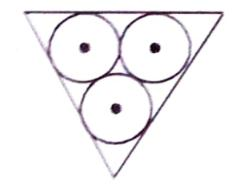
\includegraphics[width=0.75\columnwidth]{figs/figure.png}
    \label{fig:figure}
\end{figure}
\begin{multicols}{4}
\begin{enumerate}
\item $4+2\sqrt{3}$
\item $6+4\sqrt{3}$
\item $12+\frac{7\sqrt{3}}{4}$
\item $3+\frac{7\sqrt{3}}{4}$
\end{enumerate}
\end{multicols}
%
\item In a $\triangle ABC$, $a, b, c$  are the lengths of its sides and $A, B, C$ are the angles of $\triangle ABC$. The correct relation is given by
\hfill (2005)
\begin{multicols}{2}
\begin{enumerate}
\item $\brak{b-c} \sin \brak{\frac{B-C}{2}} = a \cos \brak{\frac{A}{2}}$
\item $\brak{b-c} \cos \brak{\frac{A}{2}} = a \sin \brak{\frac{B-C}{2}}$
\item $\brak{b-c} \sin \brak{\frac{B+C}{2}} = a \cos \brak{\frac{A}{2}}$
\item $\brak{b-c} \cos \brak{\frac{A}{2}} = a \sin \brak{\frac{B+C}{2}}$
\end{enumerate}
\end{multicols}
%
\item If the angles $A, B$ and $C$ of a triangle are in an arithmetic progression and if ${a}, {b}$ and ${c}$ denote the lengths of the sides opposite to $A, B$ and $C$ respectively, then the value of the expression $\frac{a}{c}\sin 2C + \frac{c}{a} \sin 2A$ is
\hfill (2010)
\begin{multicols}{4}
\begin{enumerate}
\item $\frac{1}{2}$
\item $\frac{\sqrt{3}}{2}$
\item $1$
\item $\sqrt{3}$
\end{enumerate}
\end{multicols}
%
\item Let $PQR$ be a triangle of area $\triangle$ with $a=2, b= \frac{7}{2}$ and $c=\frac{5}{2}$, where ${a}, {b}$ and ${c}$ are the lengths of the sides of the triangle opposite to the angles at $P, Q$ and $R$ respectively. Then $\frac{2\sin P - \sin 2P}{2\sin P + \sin 2P}$ equals
\hfill (2012)
\begin{multicols}{4}
\begin{enumerate}
\item $\frac{3}{4\triangle}$
\item $\frac{45}{4\triangle}$
\item $\brak{\frac{3}{4\triangle}}^2$
\item $\brak{\frac{45}{4\triangle}}^2$
\end{enumerate}
\end{multicols}
%
\item In a triangle the sum of two sides is ${x}$ and the product of the same sides is ${y}$. If $x^2-c^2=y$, where ${c}$ is the third side of the triangle, then the ratio of the inradius to the circum-radius of the triangle is
\hfill (2014)
\begin{multicols}{2}
\begin{enumerate}
\item $\frac{3y}{2\brak{x+c}}$
\item $\frac{3y}{2c\brak{x+c}}$
\item $\frac{3y}{4x\brak{x+c}}$
\item $\frac{3y}{4c\brak{x+c}}$
\end{enumerate}
\end{multicols}
     \item A $\triangle ABC$ has sides $AB=AC=5 cm$ and $BC =6 cm$. $\triangle A^{\prime}B^{\prime}C^{\prime}$ is the reflection of the $\triangle ABC$ in a line parallel to $AB$ placed at a distance of $2$ cm from $AB$, outside the $\triangle ABC$. $\triangle A^{\prime\prime}B^{\prime\prime}C^{\prime\prime}$ is the reflection of the $\triangle A^{\prime}B^{\prime}C^{\prime}$ in a line parallel $B^{\prime}C^{\prime}$ placed at a distance of $2 cm$ from $B^{\prime}C^{\prime}$ outside the $\triangle A^{\prime}B^{\prime}C^{\prime}$. Find the distance between ${A}$ and ${A^{\prime}}$.\hfill {(1978)}
     \item $ABC$ is a triangle. ${D}$ is the middle point of $BC$. If $AD$ is perpendicular to $AC$, then prove that $\cos{A}\cos{C} = \frac{2(c^{2}-a^{2}}{3ac}$.
     \hfill {(1980)}
     \item $ABC$ is a triangle with $AB=AC$. ${D}$ is any point on the side $BC$. ${E}$ and ${F}$ are points on the side $AB \text{ and } AC$, respectively, such that $DE$ is parallel to $AC, \text{ and } DF$ is parallel to $AB$. Prove that 
     \hfill {(1980)} 
     $$DF + FA + AE + ED = AB+AC$$
%
\item Let the angles $A$, $B$, $C$ of a $\triangle ABC$ be in A.P. and let $b:c=\sqrt{3}:\sqrt{2}$. Find the angle $A$. 
%
\hfill{\brak{1981}}
%
\item The ex-radii $r_1$, $r_2$, $r_3$ of $\triangle ABC$ are in H.P. Show that its sides $a$, $b$, $c$ are in A.P.
%

\hfill{\brak{1983}} 
%
\item For a $\triangle ABC$ it is given that $\cos{A}+\cos{B}+\cos{C}=\frac{3}{2}$. Prove that the triangle is equilateral. 
%
\hfill{\brak{1984}}
%
\item With usual notation, if in a $\triangle ABC$ $$\frac{b+c}{11}=\frac{c+a}{12}=\frac{a+b}{13}$$ then prove that $$\frac{\cos{A}}{7}=\frac{\cos{B}}{19}=\frac{\cos{C}}{25}.$$ 
%
\hfill{\brak{1984}}
%
%
\item In a $\triangle ABC$, the median to the side $BC$ is of length $\frac{1}{\sqrt{11-6\sqrt{3}}}$ and it divides the angle $A$ into angles $30\degree$ and $45\degree$. Find the length of the side $BC$.
%
\hfill{\brak{1985}}
%
\item If in a $\triangle ABC$, $\cos{A}\cos{B}+\sin{A}\sin{B}\sin{C}=1$, show that $a:b:c=1:1:\sqrt{2}$.
%

\hfill{\brak{1986}}
%
\item The sides of a triangle are three consecutive natural numbers and its largest angle is twice the smallest one. Determine the sides of the triangle.
%
\hfill{\brak{1991}}
%
\item In a triangle of base $a$ the ratio of the other two sides is $r\brak{<1}$. Show that the altitude of the triangle is less than or equal to $\frac{ar}{1-r^2}$.
%
\hfill{\brak{1991}}
%
%
    \item If the angles of a triangle are $30\degree$ and $45\degree$ and the included side is $(\sqrt{3} + 1) cm$, then the area of the triangle is \rule{1cm}{0.1pt}.\hfill (1988)
    \item The sides of a triangle in a given circle subtend angles $\alpha$, $\beta$, $\gamma$. The minimum value of arithmetic mean of $\cos \brak{\alpha + \frac{\pi}{2}}$, $\cos \brak{\beta + \frac{\pi}{2}}$, $\cos \brak{\gamma + \frac{\pi}{2}}$ is equal to \rule{1cm}{0.1pt}.
        \hfill{\brak{1987}}
\item $ABCD$ is a trapezium such that $AB$ and $CD$ are parallel and $BC\perp CD$. If $\angle ABD=\theta$, $BC$=$p$ and $CD$=$q$, then $AB$ is equal to
\hfill{\brak{2013}}
\begin{multicols}{4} 
\begin{enumerate}
\item $\frac{\brak{p^2+q^2}\sin\theta}{p\cos\theta+q\sin\theta}$
\item $\frac{p^2+q^2\cos\theta}{p\cos\theta+q\sin\theta}$
\item $\frac{p^2+q^2}{p\cos^2 \theta+q\sin^2 \theta}$
\item $\frac{\brak{p^2+q^2}\sin\theta}{\brak{p\cos\theta+q\sin\theta}^2}$
\end{enumerate}
\end{multicols}
\item In a $\triangle PQR$, $\angle R = \frac{\pi}{2}$. If $\tan{\frac{P}{2}}$ and $\tan{\frac{Q}{2}}$ are the roots of the equation $ax^2+bx+c=0 \;\brak{a\neq0}$ then
        \hfill{\brak{1999}}
        \begin{multicols}{4}
\begin{enumerate}
                \item $a+b=c$
                \item $b+c=a$
                \item $a+c=b$ 
                \item $b=c$
        \end{enumerate}
\end{multicols}
\item
Let O be the origin, and $\overrightarrow{OX},\overrightarrow{OY},\overrightarrow{OZ}$ be three unit vectors in the directions of the sides $\overrightarrow{QR},\overrightarrow{RP},\overrightarrow{PQ}$ respectively, of a triangle PQR.\hfill{\brak{2017}}
\begin{enumerate}
	\item $\abs{\overrightarrow{OX}\times\overrightarrow{OY}}=$
	\begin{multicols}{4}
\begin{enumerate}
		\item$\sin\brak{P+Q}$ 
		\item$\sin2R$
		\item$\sin\brak{P+R}$
		\item$\sin\brak{Q+R}$
	\end{enumerate}
\end{multicols}
%
	\item If the triangle PQR varies, then the minimum value of $\cos\brak{P+Q}+\cos\brak{Q+R}+\cos\brak{R+P}$ is
	\begin{multicols}{4}
\begin{enumerate}
		\item$\frac{-5}{3}$
		\item$\frac{-3}{2}$
		\item$\frac{3}{2}$
		\item$\frac{5}{3}$
	\end{enumerate}
\end{multicols}
	\end{enumerate}
\item $ABC$ is a triangle such that 
\hfill\brak{1990}
$$	\sin{\brak{2A+B}}=\sin{\brak{C-A}}=-\sin{\brak{B+2C}}=\frac{1}{2}
.$$
If $A$, $B$ and $C$ are in arithmetic progression, determine the values of $A$, $B$ and $C$.
\item In any $\triangle ABC$, prove that 
\hfill\brak{2000}
$$
\cot \brak{\frac{A}{2}}+\cot \brak{\frac{B}{2}}+\cot \brak{\frac{C}{2}}=\cot \brak{\frac{A}{2}}\cot \brak{\frac{B}{2}}\cot \brak{\frac{C}{2}}.
$$
\item   Let $x, y$ and $z$ be positive real numbers. Suppose $x, y$ and $z$ are the lengths of the sides of a triangle opposite to its angles $X, Y$ and $Z$, respectively. If 
\begin{align*}
	\tan\brak{\frac{X}{2}} + \tan\brak{\frac{Z}{2}} = \frac{2y}{x + y + z}
\end{align*}
    then which of the following statements is/are TRUE?
		\hfill (2020)
	\begin{multicols}{2}
    \begin{enumerate}
        \item  $2Y = X + Z$
        \item  $Y = X + 2$
	\item  $\tan\frac{X}{2} = \frac{x}{y + x}$        
	\item  $x^2 + z^2 - y^2 = xz$
    \end{enumerate}
\end{multicols}
    \item In a triangle $ABC$, let $AB = \sqrt{23}$, $BC = 3$, and $CA = 4$. Then the value of  
    \[
    \frac{\cot A + \cot C}{\cot B}
    \]  
    is \rule{1cm}{0.1pt}.
%
    \hfill (2021)
\item Let $PQRS$ be a quadrilateral in a plane, where $QR = 1$, $\angle PQR = \angle QRS = 70\degree$, $\angle PQS = 15\degree$, and $\angle PRS = 40\degree$. If $\angle RPS = \theta\degree$, $PQ = \alpha$, and $PS = \beta$, then the interval(s) that contain(s) the value of $4\alpha\beta\sin\theta\degree$ is/are
\hfill (2022)     
\begin{multicols}{4}     \begin{enumerate}
         \item $(0, \sqrt{2})$
         \item $(1, 2)$
         \item $(\sqrt{2}, 3)$
         \item $(2\sqrt{2}, 3\sqrt{2})$
    \end{enumerate} \end{multicols}
\end{enumerate}

\subsection{Olympiad}
\begin{enumerate}[label=\thesubsection.\arabic*,ref=\thesubsection.\theenumi]
    \item Let $ABCD$ be a convex quadrilateral with perpendicular diagonals. If $AB = 20$, $BC = 70$, and $CD = 90$, then what is the value of $DA$?\hfill(PRMO 2014)
    \item In a triangle with integer side lengths, one side is three times as long as a second side, and the length of the third side is $17$. What is the greatest possible perimeter of the triangle? \hfill(PRMO 2014)
    \item In a triangle $ABC$, $X$ and $Y$ are points on the segments $AB$ and $AC$, respectively, such that $ AX : XB = 1 : 2 $ and $ AY : YC = 2 : 1$. If the area of triangle $AXY$ is $10$, then what is the area of triangle $ABC$?\hfill(PRMO 2014)
    \item Let $XOY$ be a triangle with $\angle XOY = 90\degree$. Let $M$ and $N$ be the midpoints of legs $OX$ and $OY$, respectively. Suppose that $XN = 19$ and $YM = 22$. What is $XY$?

	    \hfill(PRMO 2014)
\item In $\triangle ABC$, we have $AC = BC = 7$ and $AB = 2$. Suppose that $D$ is a point on line $AB$ such that $B$ lies between $A$ and $D$ and $CD = 8$. What is the length of the segment $BD$?\hfill(PRMO 2012)
\item In rectangle $ABCD$, $AB = 5$ and $BC = 3$. Points $F$ and $G$ are on line segment $CD$ so that $DF = 1$ and $GC = 2$. Lines $AF$ and $BG$ intersect at $E$. What is the area of $\triangle ABE$?\hfill(PRMO 2012)
\item A triangle with perimeter 7 has integer side lengths. What is the maximum possible area of such a triangle?\hfill(PRMO 2012)
\item $ABCD$ is a square and $AB$ = 1. Equilateral triangles $AYB$ and $CXD$ are drawn such that $X$ and $Y$ are inside the square. What is the length of $XY$?\hfill(PRMO 2012)
    \item A $ 2 \times 3 $ rectangle and a $ 3 \times 4 $ rectangle are contained within a square without overlapping at any interior point, and the sides of the square are parallel to the sides of the two given rectangles. What is the smallest possible area of the square? 

	    \hfill(PRMO 2015)

    \item What is the greatest possible perimeter of a right-angled triangle with integer side lengths if one of the sides has length 12? \hfill(PRMO 2015)



\item In the acute-angled triangle $ABC$, let $D$ be the foot of the altitude from $A$, and $E$ be the midpoint of $BC$. Let $F$ be the midpoint of $AC$. Suppose $ \angle BAE = 40\degree $. If $ \angle DAE = \angle DFE $, what is the magnitude of $ \angle ADF $ in degrees?
	\hfill(PRMO 2015)
	\item In an equilateral triangle of side length $6$, pegs are placed at the vertices and also evenly along each side at a distance of $1$ from each other. Four distinct pegs are chosen from the $15$ interior pegs on the sides (that is, the chosen ones are not vertices of the triangle) and each peg is joined to the respective opposite vertex by a line segment. If $N$ denotes the number of ways we can choose the pegs such that the drawn line segments divide the interior of the triangle into exactly nine regions, find the sum of the squares of the digits of $N$.\hfill(IOQM 2015)		
	\item In a triangle $ABC$, let $E$ be the midpoint of $AC$ and $F$ be the midpoint of $AB$. The medians $BE$ and $CF$ intersect at $G$. Let $Y$ and $Z$ be the midpoints of $BE$ and $CF$, respectively. If the area of triangle $ABC$ is 480, find the area of triangle $GYZ$.

		\hfill(IOQM 2015)
    \item Let $X$ be the set of all even positive integers $n$ such that the measure of the angle of some regular polygon is $n$ degrees. Find the number of elements in $X$.

	    \hfill(IOQM 2015)
    \item Let $ABC$ be a triangle in the $xy$-plane, where $B$ is at the origin $\brak{0, 0}$. Let $BC$ be produced to $D$ such that $BC : CD = 1 : 1$, $CA$ be produced to $E$ such that $CA : AE = 1 : 2$, and $AB$ be produced to $F$ such that $AB : BF = 1 : 3$. Let $G\brak{32, 24}$ be the centroid of triangle $ABC$ and $K$ be the centroid of triangle $DEF$. Find the length $GK$.\hfill(IOQM 2015)
    \item A trapezium in the plane is a quadrilateral in which a pair of opposite sides are parallel. A trapezium is said to be non-degenerate if it has positive area. Find the number of mutually non-congruent, non-degenerate trapeziums whose sides are four distinct integers from the set $\cbrak{5, 6, 7, 8, 9, 10}$.\hfill(IOQM 2015)
    
\item Consider the convex quadrilateral $ABCD$. The point $P$ is the interior of $ABCD$. The following ratio equalities hold
\begin{align*}
\angle PAD: \angle PBA: \angle DPA =1:2:3 = \angle CBP: \angle BAP: \angle BPC.
\end{align*} 
prove
 that the following three lines meet in a point: the internal bisectors 
of angles $\angle ADP$ and $\angle PCB$ and the perpendicular bisector 
of segment $AB$.
\hfill(IMO 2020)
\item Three points $ X, Y, Z $ are on a straight line such that $ XY = 10 $ and $ XZ = 3 $. What is the product of all possible values of $ YZ $?\hfill(PRMO 2013)

\item Let $ AD $ and $ BC $ be the parallel sides of a trapezium $ ABCD $. Let $ P $ and $ Q $ be the midpoints of the diagonals $ AC $ and $ BD $. If $ AD = 16 $ and $ BC = 20 $, what is the length of $ PQ $?\hfill(PRMO 2013)

\item Let $ ABC $ be an equilateral triangle. Let $ P $ and $ S $ be points on $ AB $ and $ AC $, respectively, and let $ Q $ and $ R $ be points on $ BC $ such that $ PQRS $ is a rectangle. If $ PQ = \sqrt{3} PS $ and the area of $ PQRS $ is $ \frac{28}{3} $, what is the length of $ PC $?\hfill(PRMO 2013)

\item Let $ A_1, B_1, C_1, D_1 $ be the midpoints of the sides of a convex quadrilateral $ ABCD $ and let $ A_2, B_2, C_2, D_2 $ be the midpoints of the sides of the quadrilateral $ A_1B_1C_1D_1 $. If $ A_2B_2C_2D_2 $ is a rectangle with sides 4 and 6, then what is the product of the lengths of the diagonals of $ ABCD $?\hfill(PRMO 2013)


\item In a triangle $ ABC $ with $ \angle BCA = 90\degree $, the perpendicular bisector of $ AB $ intersects segments $ AB $ and $ AC $ at $ X $ and $ Y $, respectively. If the ratio of the area of quadrilateral $ BXYC $ to the area of triangle $ ABC $ is 13:18 and $ BC = 12 $, then what is the length of $ AC $?\hfill(PRMO 2013)
\item $A$ convex hexagon has the property that for any pair of opposite sides the distance between their midpoints is $\frac{\sqrt{3}}{2}$ times the sum of their lengths Show that all the hexagon's angles are equal.\hfill(IMO 2003)
\item In a triangle $ABC$, let $AP$ bisect $\angle B AC$, with $P$ on $BC$, and let $BQ$ bisect $\angle A BC$, with $Q$ on $CA$. It is known that $\angle BAC= 60\degree$ and that $AB+BP=AQ+QB$. What are the possible angles of triangle $ABC$?\hfill(IMO 2001)
\item Let $d$ be the sum of the lengths of all the diagonals of a plane convex polygon with $n$ vertices $\brak{n>3}$, and let $p$ be its perimeter. Prove that\begin{align*}                                    \ln -3<\frac{2d}{p}<\sbrak{\frac{n}{2}}\sbrak{\frac{n+1}{2}}-2,\end{align*}
		Where $\sbrak{x}$ denotes the greatest integer not exceeding $x$.  \hfill(IMO 1984)
\item $P$ is a point inside a given triangle $ABC$. $D, E, F$ are the feet of the perpendiculars from $P$ to the lines $BC, CA, AB$ respectively. Find all $P$ for which $$\frac{BC}{PD}+\frac{CA}{PE}+\frac{AB}{PF}$$ is least. \hfill(IMO  1981)
 \item The diagonals $AC$ and $CE$ of the regular hexagon $ABCDEF$ are divided by the inner points $M$ and $N$, respectively, so that \begin{align*} \frac{AM}{AC}=\frac{CN}{CE}=r.
                   \end{align*}
 Determine $r$ if $B, M$ and $N$ are collinear. \hfill(IMO  1982)
    \item Let $A$, $B$ be adjacent vertices of a regular $n$-gon $\brak{n\leq5}$ in the plane having center at $O$. A triangle $XYZ$, which is congruent to and initially coincides with $OAB$, moves in the plane in such a way that $Y$ and $Z$ each trace out the whole boundary of the polygon, $X$ remaining inside the polygon. Find the locus of $X$.\hfill(IMO  1986)

\item $ABC$ is a triangle right-angled at $A$, and $D$ is the foot of the altitude from $A$. The straight line joining the incenters of the triangles $ABD$, $ACD$ intersects the sides $AB$, $AC$ at the points $K$, $L$ respectively. $S$ and $T$ denote the areas of the triangles $ABC$ and $AKL$ respectively. Show that $S\geq 2T$.\hfill(IMO  1988)
	\item Let $ABCD$ be a convex quadrilateral such that the sides ${AB, AD, BC}$ satisfy $AB= AD + BC$. There exists a point $P$ inside the quadrilateral at a distance $h$ from the line $CD$ such that $AP= h+ AD$ and $BP= h + BC$. Show that \begin{align*}
	\frac{1}{\sqrt{h}}\geq\frac{1}{\sqrt{AD}}+\frac{1}{\sqrt{BC}}\end{align*}. \hfill(IMO  1989)
\item Prove that there exists a convex $1990$-gon with the following     two properties
\begin{enumerate}
\item All angles are equal.
\item The lengths of the 1990 sides are the numbers $1^2, 2^2, 3^2,\dots 1990^2$ in some order.\hfill(IMO  1990)
\end{enumerate}
%
\item Let $ABC$ be a triangle and $P$ an interior point of $ABC$.     Show that at least one of the angles $\angle{PAB}, \angle{PBC}, \angle{PCA}$ is less than or equal to $30\degree$.\hfill(IMO  1991)
%
\item Equilateral triangles $ABK$, $BCL$, $CDM$, $DAN$ are constructed inside the square $ABCD$. Prove that the midpoints of the four segments $KL$, $LM$, $MN$, $NK$ and the midpoints of the eight segments $AKBK$, $BL$, $CL$, $CM$, $DM$, $DN$, $AN$ are the twelve vertices of a regular dodecagon.\hfill(IMO  1977).
\item A triangle $A_1A_2A_3$ and a point $P_0 $ are given in the plane. We define $A_s
    =A_s-3$ for all $s\geq4$. We construct a set of points $P_1$, $P_2$, $P_3$ \dots, such that $P_{k+1}$ is the image of $P_k$ under a rotation with center $A_{k+1}$ through angle $120\degree$ clockwise for $\brak{k=0,1,2,3\dots}$. Prove that if $P_{1986}$=$P_0$, then the triangle $A_1A_2A_3$ is equilateral.\hfill(IMO  1986)
%
	\item Six points are chosen on the sides of an equilateral triangle $ABC$:
     $A_1$,$A_2$ on $BC$,$B_1$,$B_2$ on $CA$ and $C_1$,$C_2$ on $AB$, such that they are the vertices of a convex hexagon $A_1A_2$ $B_1B_2$ $C_1C_2$ with equal side lengths. Prove that the line $A_1B_2$,$B_1C_2$ and $C_1A_2$ are concurrent.\hfill(IMO  2005)
\item Let $P$ be a regular 2006-gon. A diagonal of $P$ is called good if its endpoints divide the boundary of $P$ into two parts, cach composed of an odd mumber of sides of P. The sides of $P$ are also called good. Suppose $P$ has been dissected into triangles by 2003 diagonals, no two of which have a common point in the interior of $P$. Find the maximum number  of isosceles triangles having two good sides that could appear in such a configuration. \hfill(IMO  2006)
\item Assign to each side $b$ of a convex polygon $P$ the maximum area of a triangle that has $b$ as a side and is contained in $P$. Show that the sum of the areas assigned to the sides of $P$ is at least twice the area of $P$.\hfill(IMO  2006)
\item Let $ABCDEF$ be a convex hexagon with $AB=BC=CD$ and $DE=EF=FA$, such that $\angle{BCD}=\angle{EFA}=\frac{\pi}{3}$. Suppose $G$ and $H$ are points in the interior of the hexagon such that $\angle{AGB}=\angle{DHE}=\frac{2\pi}{3}$. Prove that $AG+GB+GH+DH+HE\geq CF$.

	\hfill (IMO  1995)
 \item Triangle $BCF$ has a right angle at $B$. Let $A$ be the point on line $CF$ such that $FA=FB$ and $F$ lies between $A$ and $C$. Point $D$ is chosen such that $DA = DC$ and $AC$ is the bisector of $\angle DAB$. Point $E$ is chosen such that $EA= ED$ and $AD$ is the bisector of $\angle EAC$. Let $M$ be the midpoint of $CF$. Let $X$ be the point such that $AMXE$ is a parallelogram (where $AM \parallel EX$ and $AE \parallel MX)$. Prove that lines $BD, FX$, and $ME$ are concurrent.\hfill (IMO  2016)
\item $A$ convex quadrilateral $ABCD$ satisfies \begin{align*}AB.CD=BC.DA.\end{align*} Point $X$ lies inside $ABCD$ so that \begin{align*}\angle XAB=\angle XCD \text{ and } \angle XBC=\angle XDA.    \end{align*} Prove that\begin{align*}\angle BXA+\angle DXC=180\degree.\end{align*}\hfill (IMO  2018)
\item For three points $P, Q, R$ in the plane, we define $m(PQR)$ as the minimum length of the three altitudes of $\triangle PQR$. (If the points are collinear, we set $m(PQR) = 0$.)                                                                           
  Prove that for points $A, B, C, X$ in the plane,
 \hfill(IMO  1993)
\begin{align*}
                                                     m(ABC) \leq m(ABX) + m(AXC) + m(XBC).
\end{align*}
\item $ABC$ is an isosceles triangle with $AB = AC$. Suppose that  
$M$ is the midpoint of $BC$ and $O$ is the point on the line $AM$ such that $OB$ is perpendicular to $AB$.
\hfill(IMO  1994)
\begin{enumerate}
\item $Q$ is an arbitrary point on the segment $BC$ different from $B$ and $C$;                           
\item $E$ lies on the line $AB$ and $F$ lies on the line $AC$ such that $E$, $Q$, $F$ are distinct and collinear.
 
		 Prove that $OQ$ is perpendicular to $EF$ if and only if $QE=QF$.    
\end{enumerate}
%
\item Four real constants $a, b, A, B$ are given, and \begin{align*}
f\brak{\theta} = 1 - a\cos\theta - b \sin \theta     - A \cos 2\theta - B \sin 2\theta  
\end{align*}. Prove that if 
\begin{align*}f\brak{\theta} \ge 0 
	\end{align*} for all real $\theta$, then
(IMO  1977)
\begin{align*} a^{2} + b^{2} \leq 2 \text{ and } A^{2} + B^{2} \leq  1 
\end{align*}\hfill
\end{enumerate}

 %
\section{Circle}
\subsection{NCERT}
\begin{enumerate}[label=\thesubsection.\arabic*,ref=\thesubsection.\theenumi]
    \item A polygon of nine sides, each of length $2$, is inscribed in a circle. The radius of the circle is \rule{1cm}{0.1pt}. \hfill (1987) 
    \item A circle is inscribed in a equilateral triangle of a side $a$. The area of any square inscribed in this circle is \rule{1cm}{0.1pt}. \hfill (1994)  
    \item In a triangle $ABC$, $a:b:c = 4:5:6$. The ratio of the radius of the circumstances to that of the incircle is \rule{1cm}{0.1pt}. \hfill (1996) 
        \item The sum of the radii of inscribed and circumscribed circles for an $n$ sided regular polygon of side $a$, is \hfill\brak{2003}
\begin{multicols}{4}
\begin{enumerate}
        \item $\frac{a}{4} \cot{\brak{\frac{\pi}{2n}}}$         
        \item $ a \cot{\brak{\frac{\pi}{n}}}$ 
        \item $\frac{a}{2} \cot{\brak{\frac{\pi}{2n}}}$ 
        \item $ a \cot{\brak{\frac{\pi}{2n}}}$
\end{enumerate}
\end{multicols}
\item For a regular polygon, let $r$ and $R$ be the radii of the inscribed and the circumscribed circles. A false statement among the following is \hfill\brak{2010}
\begin{enumerate}
        \item There is a regular polygon with $\frac{r}{R}=\frac{1}{\sqrt{2}}$                    
        \item There is a regular polygon with $\frac{r}{R}=\frac{2}{3}$ 
        \item There is a regular polygon with $\frac{r}{R}=\frac{\sqrt{3}}{2}$ 
        \item There is a regular polygon with $\frac{r}{R}=\frac{1}{2}$
\end{enumerate}
    \item Let $A_{0}A_{1}A_{2}A_{3}A_{4}A_{5}$ be a regular hexagon inscribed in a circle of unit radius. Then the product of the lengths of the line segments $A_{0}A_{1}$,$A_{0}A_{2}$ and $A_{0}A_{4}$ is 
    \hfill{(1998)}
    \begin{multicols}{4}
    	\begin{enumerate}
    		\item ${\frac{3}{4}}$
    		\item $3\sqrt{3}$
    		\item $3$
    		\item ${\frac{3\sqrt{3}}{2}}$
    	\end{enumerate}
    \end{multicols}
    \item In a triangle $PQR$, ${P}$ is the largest angle and $\cos{P} = \frac{1}{3}$. Further the incircle of the triangle touches the sides $PQ,QR \text{ and } RP$ at ${N},{L} \text{ and } {M}$ respectively, such that the lengths of $PN, QL \text{ and } RM$ are consecutive even integers. Then possible length(s) of the side(s) of the triangle is (are)
    \hfill{(2013)}
    \begin{multicols}{4}
    	\begin{enumerate}
    		\item $16$
    		\item $24$
    		\item $18$
    		\item $22$
    	\end{enumerate}
    \end{multicols}
    \item In a triangle $XYZ$, let $x,y,z$ be the lengths of sides opposite to angles ${X},{Y},{Z} \text{ and } 2s = x+y+z$. If $${\frac{s-x}{4}}={\frac{s-y}{3}}={\frac{s-z}{2}}$$ and area of the incircle of the triangle $XYZ$ is ${\frac{8\pi}{3}},$
    \hfill{(2016)}
    \begin{enumerate}
    	\item area of the triangle is $6\sqrt{6}$
    	\item the radius of circumcirle of $XYZ$ is ${\frac{35\sqrt{6}}{6}}$
    	\item $\sin\frac{X}{2}\sin\frac{Y}{2}\sin\frac{Z}{2} = \frac{4}{35}$
    	\item $\sin^{2}\brak{\frac{X+Y}{2}}$ = $\frac{3}{5}$
    \end{enumerate}
    \item In a triangle $PQR$, let $\angle PQR = 30\degree$ and the sides $PQ \text{ and } QR$ have lengths $10\sqrt{3}$ and $10$ respectively. Then which of the following statements is (are)  TRUE?
    \hfill{(2018)}
    \begin{enumerate}
    	\item $\angle QPR = 45\degree$
    	\item the area of the triangle $PQR$ is $25\sqrt{3}$ and $\angle QRP = 120\degree$
    	\item the radius of the incircle of triangle $PQR$ is $10\sqrt{3}-15$
    	\item the radius of circumcirle $PQR$ is $100\pi$
    \end{enumerate}
    \item In a non-right-angle triangle $\triangle PQR$, let $p,q,r$ denote the lengths of the sides opposite to the angles at ${P},{Q},{R}$ respectively. The median from ${R}$ meets the side $PQ$ at ${S}$, the perpendicular from ${P}$ meets the side $QR$ at ${E}$, $RS \text{ and } PE$ intersect at ${O}$. If $p = \sqrt{3}$, $q = 1$ and the radius of the circumcircle at $\triangle PQR$ equals $1$, then which of the following options is (are) correct.
    \hfill{(2018)}
    \begin{enumerate}
    	\item Radius of incircle of $\triangle PQR$ = $\frac{\sqrt{3}}{2}\brak{2-\sqrt{3}}$
    	\item Area of $\triangle SOE = \frac{\sqrt{3}}{12}$
    	\item Length of $OE = \frac{1}{6}$
    	\item Length of $RS = \frac{\sqrt{7}}{2}$
    \end{enumerate}
\item Which of the following pieces of data does NOT uniquely determine an acute-angled triangle $\triangle ABC$ (${R}$ being the radius of the circumcircle)?
\hfill (2002)
		\begin{multicols}{4}
\begin{enumerate}
\item $a, \sin A, \sin B$
\item $a, b, c$
\item $a, \sin B, R$
\item $a, \sin A, R$
\end{enumerate}
    \end{multicols}
\item One angle of an isosceles $\triangle$ is $120\degree$ and radius of its incircle $= \sqrt{3}$. Then the area of the triangle in sq. units is 
\hfill (2006)
		\begin{multicols}{4}
\begin{enumerate}
\item $7+12\sqrt{3}$
\item $12-7\sqrt{3}$
\item $12+7\sqrt{3}$
\item $4\pi$
\end{enumerate}
    \end{multicols}
%
\item Let $ABCD$ be a quadrilateral with area $18$, with side $AB$ parallel to the side $CD$ and $2AB = CD$. Let $AD$ be perpendicular to $AB$ and $CD$. If a circle is drawn inside the quadrilateral $ABCD$ touching all the sides, then the radius is
\hfill (2007)
		\begin{multicols}{4}
\begin{enumerate}
\item $3$
\item $2$
\item $\frac{3}{2}$
\item $1$
\end{enumerate}
\end{multicols}
%
     	\item If a triangle is inscribed in a circle, then the product of any two sides of the triangle is equal to the product of the diameter and perpendicular distance of the third side from the opposite vertex. Prove the above statement.
     \hfill {(1979)}
     	\item Find the area of the smaller part of a disc of radius $10 cm$, cut off by a chord $AB$ which subtends an angle of $22\frac{1}{2} \degree$ at the circumference.
     \hfill {(1980)}
 \item Let $ABC$ be the triangle with $AB = 1, AC = 3$ and $\angle BAC=\frac{\pi}{2}$. If a circle of radius $r > 0$ touches the sides $AB, AC$ and also touches internally the circumcircle of the triangle $ABC$, then the value of $r$ is\rule{1cm}{0.1pt}.
	\hfill (2022)
\item Let $G$ be a circle of radius $R > 0$. Let $G_1, G_2, \dots, G_n$ be $n$ circles of equal radius $r > 0$. Suppose each of the $n$ circles $G_1, G_2, \dots, G_n$ touches the circle $G$ externally. Also, for $i = 1, 2, \dots, n - 1$, the circle $G_i$ touches $G_{i+1}$ externally, and $G_n$ touches $G_1$ externally. Then, which of the following statements is/are TRUE?
\hfill (2022)     
\begin{multicols}{2}     \begin{enumerate}
         \item If $n = 4$, then $(\sqrt{2} - 1)r < R$.
         \item If $n = 5$, then $r < R$.
         \item If $n = 8$, then $(\sqrt{2} - 1) r < R$.
         \item If $n = 12$, then $\sqrt{2} (\sqrt{3} + 1) r > R$.
    \end{enumerate} \end{multicols}
\item Consider an obtuse angled triangle $ABC$ in which the difference between the largest and the smallest angle is $\frac{\pi}{2}$ and whose sides are in arithmetic progression. Suppose that the vertices of this triangle lie on a circle of radius 1.
\hfill (2023)
\begin{enumerate}
\item Let $a$ be the area of the triangle $ABC$. Then the value of $(64a)^2$ is
\rule{1cm}{0.1pt}.
\item The in radius of the triangle $ABC$ is
\rule{1cm}{0.1pt}.
\end{enumerate}
%
\item Let $A_1, A_2, A_3, \dots, A_8$ be the vertices of a regular octagon that lie on a circle of radius 2. Let $P$ be a point on the circle, and let $PA_i$ denote the distance between the points $P$ and $A_i$ for $i = 1,2, \dots, 8$. If $P$ varies over the circle, then the maximum value of the product $PA_1 \cdot PA_2 \cdot PA_3 \cdots PA_8$ is
\rule{1cm}{0.1pt}.
\hfill (2023)



\end{enumerate}

\subsection{JEE}
\begin{enumerate}[label=\thesubsection.\arabic*,ref=\thesubsection.\theenumi]
    \item A polygon of nine sides, each of length $2$, is inscribed in a circle. The radius of the circle is \rule{1cm}{0.1pt}. \hfill (1987) 
    \item A circle is inscribed in a equilateral triangle of a side $a$. The area of any square inscribed in this circle is \rule{1cm}{0.1pt}. \hfill (1994)  
    \item In a triangle $ABC$, $a:b:c = 4:5:6$. The ratio of the radius of the circumstances to that of the incircle is \rule{1cm}{0.1pt}. \hfill (1996) 
        \item The sum of the radii of inscribed and circumscribed circles for an $n$ sided regular polygon of side $a$, is \hfill\brak{2003}
\begin{multicols}{4}
\begin{enumerate}
        \item $\frac{a}{4} \cot{\brak{\frac{\pi}{2n}}}$         
        \item $ a \cot{\brak{\frac{\pi}{n}}}$ 
        \item $\frac{a}{2} \cot{\brak{\frac{\pi}{2n}}}$ 
        \item $ a \cot{\brak{\frac{\pi}{2n}}}$
\end{enumerate}
\end{multicols}
\item For a regular polygon, let $r$ and $R$ be the radii of the inscribed and the circumscribed circles. A false statement among the following is \hfill\brak{2010}
\begin{enumerate}
        \item There is a regular polygon with $\frac{r}{R}=\frac{1}{\sqrt{2}}$                    
        \item There is a regular polygon with $\frac{r}{R}=\frac{2}{3}$ 
        \item There is a regular polygon with $\frac{r}{R}=\frac{\sqrt{3}}{2}$ 
        \item There is a regular polygon with $\frac{r}{R}=\frac{1}{2}$
\end{enumerate}
    \item Let $A_{0}A_{1}A_{2}A_{3}A_{4}A_{5}$ be a regular hexagon inscribed in a circle of unit radius. Then the product of the lengths of the line segments $A_{0}A_{1}$,$A_{0}A_{2}$ and $A_{0}A_{4}$ is 
    \hfill{(1998)}
    \begin{multicols}{4}
    	\begin{enumerate}
    		\item ${\frac{3}{4}}$
    		\item $3\sqrt{3}$
    		\item $3$
    		\item ${\frac{3\sqrt{3}}{2}}$
    	\end{enumerate}
    \end{multicols}
    \item In a triangle $PQR$, ${P}$ is the largest angle and $\cos{P} = \frac{1}{3}$. Further the incircle of the triangle touches the sides $PQ,QR \text{ and } RP$ at ${N},{L} \text{ and } {M}$ respectively, such that the lengths of $PN, QL \text{ and } RM$ are consecutive even integers. Then possible length(s) of the side(s) of the triangle is (are)
    \hfill{(2013)}
    \begin{multicols}{4}
    	\begin{enumerate}
    		\item $16$
    		\item $24$
    		\item $18$
    		\item $22$
    	\end{enumerate}
    \end{multicols}
    \item In a triangle $XYZ$, let $x,y,z$ be the lengths of sides opposite to angles ${X},{Y},{Z} \text{ and } 2s = x+y+z$. If $${\frac{s-x}{4}}={\frac{s-y}{3}}={\frac{s-z}{2}}$$ and area of the incircle of the triangle $XYZ$ is ${\frac{8\pi}{3}},$
    \hfill{(2016)}
    \begin{enumerate}
    	\item area of the triangle is $6\sqrt{6}$
    	\item the radius of circumcirle of $XYZ$ is ${\frac{35\sqrt{6}}{6}}$
    	\item $\sin\frac{X}{2}\sin\frac{Y}{2}\sin\frac{Z}{2} = \frac{4}{35}$
    	\item $\sin^{2}\brak{\frac{X+Y}{2}}$ = $\frac{3}{5}$
    \end{enumerate}
    \item In a triangle $PQR$, let $\angle PQR = 30\degree$ and the sides $PQ \text{ and } QR$ have lengths $10\sqrt{3}$ and $10$ respectively. Then which of the following statements is (are)  TRUE?
    \hfill{(2018)}
    \begin{enumerate}
    	\item $\angle QPR = 45\degree$
    	\item the area of the triangle $PQR$ is $25\sqrt{3}$ and $\angle QRP = 120\degree$
    	\item the radius of the incircle of triangle $PQR$ is $10\sqrt{3}-15$
    	\item the radius of circumcirle $PQR$ is $100\pi$
    \end{enumerate}
    \item In a non-right-angle triangle $\triangle PQR$, let $p,q,r$ denote the lengths of the sides opposite to the angles at ${P},{Q},{R}$ respectively. The median from ${R}$ meets the side $PQ$ at ${S}$, the perpendicular from ${P}$ meets the side $QR$ at ${E}$, $RS \text{ and } PE$ intersect at ${O}$. If $p = \sqrt{3}$, $q = 1$ and the radius of the circumcircle at $\triangle PQR$ equals $1$, then which of the following options is (are) correct.
    \hfill{(2018)}
    \begin{enumerate}
    	\item Radius of incircle of $\triangle PQR$ = $\frac{\sqrt{3}}{2}\brak{2-\sqrt{3}}$
    	\item Area of $\triangle SOE = \frac{\sqrt{3}}{12}$
    	\item Length of $OE = \frac{1}{6}$
    	\item Length of $RS = \frac{\sqrt{7}}{2}$
    \end{enumerate}
\item Which of the following pieces of data does NOT uniquely determine an acute-angled triangle $\triangle ABC$ (${R}$ being the radius of the circumcircle)?
\hfill (2002)
		\begin{multicols}{4}
\begin{enumerate}
\item $a, \sin A, \sin B$
\item $a, b, c$
\item $a, \sin B, R$
\item $a, \sin A, R$
\end{enumerate}
    \end{multicols}
\item One angle of an isosceles $\triangle$ is $120\degree$ and radius of its incircle $= \sqrt{3}$. Then the area of the triangle in sq. units is 
\hfill (2006)
		\begin{multicols}{4}
\begin{enumerate}
\item $7+12\sqrt{3}$
\item $12-7\sqrt{3}$
\item $12+7\sqrt{3}$
\item $4\pi$
\end{enumerate}
    \end{multicols}
%
\item Let $ABCD$ be a quadrilateral with area $18$, with side $AB$ parallel to the side $CD$ and $2AB = CD$. Let $AD$ be perpendicular to $AB$ and $CD$. If a circle is drawn inside the quadrilateral $ABCD$ touching all the sides, then the radius is
\hfill (2007)
		\begin{multicols}{4}
\begin{enumerate}
\item $3$
\item $2$
\item $\frac{3}{2}$
\item $1$
\end{enumerate}
\end{multicols}
%
     	\item If a triangle is inscribed in a circle, then the product of any two sides of the triangle is equal to the product of the diameter and perpendicular distance of the third side from the opposite vertex. Prove the above statement.
     \hfill {(1979)}
     	\item Find the area of the smaller part of a disc of radius $10 cm$, cut off by a chord $AB$ which subtends an angle of $22\frac{1}{2} \degree$ at the circumference.
     \hfill {(1980)}
 \item Let $ABC$ be the triangle with $AB = 1, AC = 3$ and $\angle BAC=\frac{\pi}{2}$. If a circle of radius $r > 0$ touches the sides $AB, AC$ and also touches internally the circumcircle of the triangle $ABC$, then the value of $r$ is\rule{1cm}{0.1pt}.
	\hfill (2022)
\item Let $G$ be a circle of radius $R > 0$. Let $G_1, G_2, \dots, G_n$ be $n$ circles of equal radius $r > 0$. Suppose each of the $n$ circles $G_1, G_2, \dots, G_n$ touches the circle $G$ externally. Also, for $i = 1, 2, \dots, n - 1$, the circle $G_i$ touches $G_{i+1}$ externally, and $G_n$ touches $G_1$ externally. Then, which of the following statements is/are TRUE?
\hfill (2022)     
\begin{multicols}{2}     \begin{enumerate}
         \item If $n = 4$, then $(\sqrt{2} - 1)r < R$.
         \item If $n = 5$, then $r < R$.
         \item If $n = 8$, then $(\sqrt{2} - 1) r < R$.
         \item If $n = 12$, then $\sqrt{2} (\sqrt{3} + 1) r > R$.
    \end{enumerate} \end{multicols}
\item Consider an obtuse angled triangle $ABC$ in which the difference between the largest and the smallest angle is $\frac{\pi}{2}$ and whose sides are in arithmetic progression. Suppose that the vertices of this triangle lie on a circle of radius 1.
\hfill (2023)
\begin{enumerate}
\item Let $a$ be the area of the triangle $ABC$. Then the value of $(64a)^2$ is
\rule{1cm}{0.1pt}.
\item The in radius of the triangle $ABC$ is
\rule{1cm}{0.1pt}.
\end{enumerate}
%
\item Let $A_1, A_2, A_3, \dots, A_8$ be the vertices of a regular octagon that lie on a circle of radius 2. Let $P$ be a point on the circle, and let $PA_i$ denote the distance between the points $P$ and $A_i$ for $i = 1,2, \dots, 8$. If $P$ varies over the circle, then the maximum value of the product $PA_1 \cdot PA_2 \cdot PA_3 \cdots PA_8$ is
\rule{1cm}{0.1pt}.
\hfill (2023)



\end{enumerate}

\subsection{Olympiad}
\begin{enumerate}[label=\thesubsection.\arabic*,ref=\thesubsection.\theenumi]
   % 
    \item Let $ABCD$ be a unit square. Suppose $M$ and $N$ are points on $BC$ and $CD$, respectively, such that the perimeter of triangle $MCN$ is $2$. Let $O$ be the circumcenter of triangle $MAN$, and $P$ be the circumcenter of triangle $MON$. If $\left(\frac{OP}{OA}\right)^2 = \frac{m}{n}$ for some relatively prime positive integers $m$ and $n$, find the value of $m + n$.\hfill(IOQM 2015)
    
    \item In triangle  $ABC$, point $ A_1 $ lies on side $ BC $ and point $B_1$ lies on side $ AC $. Let  $P$ and $ Q $ be points on segments 
$AA_1$ and $BB_1 $, respectively, such that   $PQ \parallel AB$.
Let
 $P_1$ be a point on line  $PB_1$ such that $B_1$ lies strictly between 
$P$ and $P_1$, and $\angle PP_1C$ = $\angle BAC$. Similarly, let $Q_1$ 
be a point on line $QA_1$ such that $A_1$ lies strictly between $Q$ and 
$Q_1$, and $ \angle CQ_1Q$ = $\angle CBA $.
Prove that points $P, Q, P_1,$ and $Q_1$ are concyclic.
\hfill(IMO 2019)


\item Let $D$ be an interior point of the acute triangle $ABC$ with $AB > AC$ so that $\angle DAB = \angle CAD$. The point $E$ on the segment $AC$ satisfies $\angle ADE=\angle BCD$, the point $F$ on the segment $AB$ satisfies $\angle FDA=\angle DBC$, and the point $X$ on the line $AC$ satisfies $CX=BX$. let $O_{1}$ and $O_{2}$ be the circumcentres of the triangles $ADC$ and $EXD$, respectively. Prove that the lines $BC,EF$ and $O_{1} O_{2}$ are concurrent.
 \hfill(IMO 2021)

\item $ABCD$ is cyclic. The feet of the perpendicular from $D$ to the lines $AB$, $BC$, $CA$ are $P, Q,R $ respectivel$y$. Show that the angle bisectors of $ ABC$ and $CDA$ meet on the line $AC$ iff $RP = RQ$.\hfill(IMO 2003)
%
\item In the convex quadrilateral $ABCD$, the diagonals $AC$ and $BD$ are perpendicular and the opposite sides $AB$ and $DC$ are not parallel. Suppose that the point $P$, where the perpendicular bisectors of $AB$and $DC$ meet, is inside $ABCD$. Prove that $ABCD$ is a cyclic quadrilateral if and only if the triangles $ABP$ and $CDP$ have equal areas.

	\hfill(IMO  1998) 
\item Consider five points $A,B,C,D$ and $E$ such that $ABCD$ is a parallelogram and $BCED$ is a cyclic quadrilateral. Let $l$ be a line passing through $A$. Suppose that $l$ intersts the interior of the segment $DC$ at $F$ and intersects line $BC$ at $G$. Suppose also that $EF=EG=EC$. Prove that $l$ is the bisector of angle $DAB$.\hfill(IMO  2007)
		
\item Let $P$ be a point inside triangle $ABC$ such     that                                         
\begin{align*}                                      
	\angle{APB}-\angle{ACB}=\angle{APC}-\angle{ BC}.
 \end{align*}                                       
Let $D$, $E$ be the incenters of triangles $APB$, $APC$, respectively. Show that $AP$, $BD$, $CE$ meet at a point.\hfill(IMO  1996)
\item Let $ABCDEF$ be a convex hexagon such that $A$ is parallel to $DE$, $BC$ is parallel to $EF$, and $CD$ is parallel to $FA$. Let $R_A$, $R_C$, $R_E$ denote the circumradii of triangles $FAB$, $BCD$, $DEF$, respectively, and let $P$ denote the perimeter of the hexagon. Prove that            \hfill(IMO  1996)
\begin{align*}                                            R_A+R_C+R_E\geq\frac{p}{2}.  
\end{align*}
\item The angle at $A$ is the smallest angle of triangle $ABC$. The point $B$ and $C$ divide the circumcircle of the triangle into two arcs. Let $U$ be an interior point of the arc between $B$ and $C$ which does not contain $A$. The perpendicular bisectors of  $AB$ and $AC$ meet the line $AU$ at $V$ and $W$, respctively. The lines $BV$ and $CW$ meet at $T$. Show that
\hfill(IMO  1997)
 \begin{align*}
AU=TB+TC.
 \end{align*}                                   
\item Let $P=A_1A_2 \dots A_k$ be a convex polygon in the plane. The vertices $A_1, A_2,\dots A_k $ have integral coordinates and lie on a circle. Let $S$ be the area of $P$. An odd positive integer $n$ is given such that the squares of the side lengths of $P$ are integers divisible by $n$. Prove that $2S$ is an integer divisible by $n$.\hfill(IMO  2016)
\item Let $I$ be the circumcircle of acute-angled triangle $ABC$. Points $D$ and $E$     lie on segments $AB$ and $AC$ respectively, such that $AD=AE$. The perpendicular bisectors of $BD$ and $CE$ intersect the minor arcs $AB$ and $AC$ of $I$ at points $F$ and $G$ respectively. Prove that the lines $DE$ and $FG$ are parallel (or are the same line).\hfill (IMO  2018)
\item In the plane let $C$ be a circle, $L$ a line  tangent to the circle $C$, and $M$ a point on $L$. Find the locus of all points $P$ with the following property: there exists two points $Q,R$ on $L$ such that $M$ is the midpoint of $QR$ and $C$ is the inscribed circle of triangle $PQR$.  \hfill(IMO  1992)
\item Let $D$ be a point inside acute triangle $ABC$ such that $\angle ADB$ $=$ $\angle ACB$ $+$ $\pi/2$ and $AC \cdot BD = AD \cdot BC$.
 
\begin{enumerate}
\item Calculate the ratio $(AB \cdot CD) / (AC \cdot B)$.
\item Prove that the tangents at $C$ to the circumcircles of $\triangle ACD$ and $\triangle BCD$ are perpendicular. \hfill(IMO  1993)
\end{enumerate}
\item In a triangle $ABC$, let $I$ denote the incenter. Let the lines $AI$, $BI$, and $CI$ intersect the incircle at $P$, $Q$, and $R$, respectively. If $\angle BAC = 40\degree$, what is the value of $\angle QPR$ in degrees?\hfill(PRMO 2014)
\item $AB$ is tangent to the circles $CAMN$ and $NMBD$. $M$ lies between $C$ and $D$ on the line $CD$, and $CD$ is parallel to $AB$. The chords $NA$ and $CM$ meet at $P$; the chords $NB$ and $MD$ meet at $Q$. The rays $CA$ and $DB$ meet at $E$. Prove that $PE = QE$.

	\hfill(IMO 2000)
\item $O$ and $I$ are the circumcentre and incentre of $\triangle ABC$ respectively. Suppose $O$ lies in the interior of $\triangle ABC$ and $I$ lies on the circle passing through $B$, $O$, and $C$. What is the magnitude of $\angle BAC$ in degrees?\hfill(PRMO 2012)
    \item In rectangle $ ABCD $, $ AB = 8 $ and $ BC = 20 $. Let $ P $ be a point on $ AD $ such that $ \angle BPC = 90\degree $. If $ r_1, r_2, r_3 $ are the radii of the incircles of triangles $ APB, BPC $, and $ CPD $, what is the value of $ r_1 + r_2 + r_3 $? \hfill(PRMO 2015)
\item The circle $ \omega $ touches the circle $ \Omega $ internally at $ P $. The center $ O $ of $ \Omega $ is outside $ \omega $. Let $XY$ be a diameter of $ \Omega $ which is also tangent to $ \omega $. Assume $ PY > PX $. Let $ PY $ intersect $ \omega $ at $ Z $. If $ YZ = 2PZ $, what is the magnitude of $ \angle LPYX $ in degrees? 

	\hfill(PRMO 2015)
\item
 Let $I$ be the incentre of acute triangle $ABC$ with $AB$ $\neq AC$. 
The incircle $\omega$ of $ABC$ is tangent to sides $ BC$, $CA$, and $AB$
 at points $D$,  $E$, and $F$, respectively. 
The line 
through $D$ perpendicular to $EF$ meets $\omega$ again at $R$. Line $AR$
 meets $\omega$ again at $P$. The circumcircles of triangles $PCE$ and 
$PBF$ meet again at $Q$.
Prove that lines $DI$ and $PQ$ meet on the line through $ A$ that is perpendicular to $AI$.
\hfill(IMO 2019)
\item Let $r$ be a circle with centre $I$, and $ABCD$ a convex quadrilateral such that each of the segments $AB,BC,CD$ and $DA$ is a tangent to $r$. Let $\Omega$ be the circumcircle of the triangle $AIC$. The extension of $BA$ beyond $A$ meets $\Omega$ at $X$, and the extension of $BC$ beyond $C$ meets $\Omega$ at $Z$. The extensions of $AD$ and $CD$ beyond $D$ meet $\Omega$ at $Y$ and $T$, respectively. Prove that
\begin{align*}
    AD+DT+TX+XA=CD+DY+YZ+ZC
\end{align*}
 \hfill(IMO 2021)
 \item
Let $ABCDE$  be a convex pentagon such that  $BC = DE$.  Assume that there is a point  $T$  inside  $ABCDE$ with  $TB = TD$,  $TC = TE$  and  $\angle{ABT} = \angle{TEA}$.  Let line  $AB$  intersect 
lines $CD$  and  $CT$  at points  $P$  and $Q$,  respectively. Assume that the points  $P, B, A, Q$  occur on their line in that order. Let line  $AE$  intersect lines  $CD$  and  $DT$  at points  $R$  and  $S$,  respectively. Assume 
that the points $ R, E, A, S $ occur on their line in that order. Prove that the points $ P, S, Q, R $ lie on a circle. \hfill(IM0 2022)
\item
Let  $ABC$ be an acute-angled triangle with  $AB \leq AC$. Let $\Omega$  be the circumcircle of  $ABC$.  Let  $S$ be the midpoint of the arc  $CB$  of  $\Omega$ containing $A$.  The perpendicular from $A$  to  $BC$ meets  $BS$  at  $D$  and meets  $\Omega$  again at$ E \neq A$. The line through $
D$ parallel to  $BC$  meets line  $BE$ at  $L$.  Denote the circumcircle of triangle  $BDL$  by  $\omega$.  Let  $\omega$  meet  $\Omega$  again at  $P \neq B$. Prove that the line tangent to $\omega$ at  $P$  meets line $BS$  on the internal angle bisector of  $\angle{BAC}$. \hfill(IMO 2023)
\item
Let  $ABC$  be an equilateral triangle. Let $A_{1}, B_{1}, C_{1}$  be interior points of  $ABC$  such that $ BA_{1} = A_{1}C, CB_{1} = B_{1}A, AC_{1} = C_{1}B,$  and $\angle{BAC} + \angle{CB_{1}A} + \angle{AC_{1}B} = 480^{\circ}.$  Let $ BC_{1}$ and $CB_{1}$  meet at $A_{2}$,  let  $CA_{1}$ and  $A
C_{1}$  meet at  $B_{2}$,  and let  $AB_{1}$ and  $BA_{1}$  meet at  $C_{2}$. Prove that if triangle  $A_{1}B_{1}C_{1}$  is scalene, then the three circumcircles of triangles $AA_{1}A_{2}, BB_{1}B_{2}$  and  $CC_{1}C_{2}$ all pass through two common points.
$\brak{\text{Note: no 2 sides have equal length.}}$ \hfill(IMO 2023)
\item
Let  $ABC$  be a triangle with $ AB \leq AC \leq BC $.  Let the incentre and incircle of triangle   $ABC$  be  $I$ and  $\omega$, respectively. Let $X$ be the point on line  $BC$  different from  $C$  such that the line   through  $X$  parallel to  $AC$  is tangent to  $\omega$.  Similarly, let  $
Y$ be the point on line  $BC$  different from  $B$  such that the line through  $Y$ parallel to  $AB$  is tangent to  $\omega$.  Let $AI$  intersect the circumcircle of  triangle $ABC$  again at  $P \neq A$. Let  $K$  and $L$  be the midpoints of  $AC$  and  $AB$,  respectively.  Prove that  $\angle{KIL} + \angle{YPX} = 180^{\circ}.$ 

\hfill(IMO 2024)
\item In a triangle $ ABC $, let $ H $, $ I $, and $ O $ be the orthocenter, incenter, and circumcenter, respectively. If the points $ B $, $ H $, $ I $, and $ C $ lie on a circle, what is the magnitude of $ \angle BOC $ in degrees?\hfill(PRMO 2013)
\item Let $ S $ be a circle with center $ O $. A chord $ AB $, not a diameter, divides $ S $ into two regions $ R_1 $ and $ R_2 $. Let $ S_1 $ be a circle with center in $ R_1 $ touching $ AB $, the circle $ S $ internally. Let $ S_2 $ be a circle with center in $ R_2 $ touching $ AB $ at $ Y $, the circle $ S $ internally, and passing through the center of $ S $. The point $ X $ lies on the diameter passing through the center of $ S_2 $, and $ \angle YXO = 30\degree $. If the radius of $ S_2 $ is 100, then what is the radius of $ S $?\hfill(PRMO 2013)
\item $BC$ is a diameter of a circle with center $O$. $A$ is any point on the circle with $\angle AOC > 60\degree$. $EF$ is the chord which is the perpendicular bisector of $AO$. $D$ is the midpoint of the minor arc $AB$. The line through $O$ parallel to $AD$ meets $AC$ at $J$. Show that $J$ is the incenter of triangle $CEF$.\hfill(IMO 2002)
\item Let $ABCD$ be a convex quadrilateral such that the line $CD$ is a  tangent to the circle on $AB$ as diameter. Prove that the line $AB$ is a tangent to the  circle on $CD$ as diameter if and only if the lines $BC$ and $AD$ are parallel.\hfill(IMO 1984)
\item let $A$ be one of the two distinct points of intersection of two unequal coplanar tangents to the circles $C_1$ and $C_2$ with centers $ O_1$ and $O_2$, respectively. One of the common tangents to the circles touches $C_1$ at $P_1$ and $C_2$ at $P_2$, while the other touches $C_1$ at $Q_1$ and $C_2$ at $Q_2$.  Let $M_1$ be the midpoint of $P_1Q_1$, $M_2$ be the midpoint of $P_2Q_2$. Prove that $\angle O_1AO_2 =\angle M_1AM_2$.\hfill(IMO 1983)
     \item $A$ circle has center on the side $AB$ of the cyclic quadrilateral $ABCD$. The other three sides are tangent to the circle. Prove that $AD+BC = AB$.\hfill(IMO 1985)
\item A circle with center $O$ passes through the vertices $A$ and $C$ of triangle $ABC$ and intersects the segments $AB$ and $BC$ again at distinct points $K$ and $N$ respectively. The circumscribed circle of the triangle $ABC$ and $EBN$ intersect at exactly two distinct points $B$ and $M$. Prove that angle $OMB$ is a right angle.\hfill(IMO 1985)
\item Three congruent circles have a common point $O$ and lie inside     a given triangle. Each circle touches a pair of sides of the triangle. Prove that the incenter and the circumcenter of the triangle and   the point $O$  are collinear. \hfill(IMO  1981)     
\item A non-isosceles triangle $A_1 A_2 A_3$ is given with sides $a_1,a_2,a_3$ ($a_i$ is the side opposite $A_i$). For all $i = 1, 2, 3, M_i$ is the midpoint of side $a_i$ and $T_i$ is the point where     the incircle touches side $a_i$. Denote by $S_i$ the reflection of $T_i$ in the interior bisector of angle $A_i$. Prove that the lines $M_1S_1$, $ M_2S_2$ and $M_3S_3$ are concurrent.\hfill(IMO  1982)
    \item In an acute-angled triangle $ABC$ the interior bisector of the angle $A$ intersects $BC$ at $L$ and intersects the circumcircle of $ABC$ again at $N$. From point $L$ perpendiculars are drawn to $AB$ and $AC$, the feet of these perpendiculars being $K$ and $M$ respectively. Prove that the quadrilateral $AKNM$ and the triangle $ABC$ have equal areas.

	    \hfill(IMO  1987)
    \item Consider two coplanar circles of radii $R$ and $r$ $\brak{R > r}$ with the same center. Let $P$ be a fixed point on the smaller circle and $B$ a variable point on the larger circle. The line $BP$ meets the larger circle again at $C$. The perpendicular $l$ to $BP $ at $P$ meets the smaller circle again at $A$. (If $l$ is tangent to the circle at $P$ then $A = P$).
\hfill(IMO  1988)
\begin{enumerate}
	\item  Find the set of values of $BC^2+CA^2+AB^2$ 
	\item  Find the locus of the midpoint of $BC$.
\end{enumerate}
\item  Let the excircle of triangle $ABC$ opposite the vertex $A$ be tangent to the side $BC$ at the point $A_1$. Define the points $B_1$ on $CA$ and $C_1$ on $AB$ analogously, using the excircles opposite $B$ and $C$ respectively. Suppose that the circumcentre of triangle $A_1B_1C_1$, lies on the circumcircle of triangle $ABC$. Prove that triangle $ABC$ is right-angled. 
	(The excircle of triangle $ABC$ opposite the vertex $A$ is the circle that is tangent to the line segment $BC$, to the ray $AB$ beyond $B$, and to the ray $AC$ beyond $C$. The excircles opposite $B$ and $C$ are similarly defined. \hfill(IMO  2013)
\item  Convex quadrilateral $ABCD$ has $\angle ABC= \angle CDA = 90 \degree$. Point $H$ is the foot of the perpendicular from $A$ to $BD$. Points $S$ and $T$ lie on sides $AB$ and $AD$ respectively, such that $H$ lies inside triangle $SCT$ and $\angle CHS- \angle CSB = 90 \degree, \angle THC- \angle DTC = 90\degree$.
	Prove that line $BD$ is tangent to the circumcircle of triangle $TSH$.
	\hfill(IMO  2014)
\item   Points $P$ and $Q$ lie on side $BC$ of acute-angled triangle $ABC$ so that $\angle PAB= \angle BCA$ and $\angle CAQ=\angle ABC.$ Points $M$ and $N$ lie on lines $AP$ and $AQ,$ respectively, such that $P$ is the midpoint of $AM,$ and $Q$ is the midpoint of $AN.$ Prove that lines $BM$ and $CN$ intersect on circumcircle of triangle $ABC$ \hfill(IMO  2014)
\item   Let $ABC$ be an acute triangle with $AB > AC$. Let $I$ be its circumcircle, $H$ its orthocentre, and $F$ the foot of the altitude from $A$. Let $M$ be the midpoint of $BC$. Let $Q$ be the point on $T$ such that $\angle HQA= 90$, and let $K$ be the point on $T$ such that $\angle HKQ=90\degree.$ Assume that the points $ A, B, C, K$ and $Q$ are all different, and lie on $T$ in this order.
	Prove that the circumcircles of triangles $KQH$ and $FKM$ are tangent to each other. \hfill(IMO 2015)
\item  Triangle $ABC$ has circumcircle $\Omega$ and circumcentre $O$. A circle $T$ with centre $A$ intersects the segment $BC$ at points $D$ and $E$, such that $B, D, E $ and $C$ are all different and lie on line $BC$ in this order. Let $F$ and $G$ be the points of intersection of $T$ and $\Omega$ such that $A, F, B, C$ and $G$ lie on $\Omega$ in this order. Let $K $ be the second point of intersection of the circumcircle of triangle $BDF$ and the segment $AB$. Let $L$ be the second point of intersection of the circumcircle of triangle $CGE$ and the segment $CA$.
	Suppose that the lines $FK$ and $GL$ are different and intersect at the point $X$. Prove that $X$ lies on the line $AO$. \hfill(IMO  2015)
\item In an acute-angled triangle $ABC$, the internal bisector of angle $A$ meets the circumcircle of the triangle again at $A_1$. Points $B_1$ and $C_1$ are defined similarly. Let $A_0$ be the point of intersection of the line $AA_1$ with the external bisectors of angles $B$ and $C$. Points $B_0$ and $C_0$ are defined similarly. Prove that
\begin{enumerate}
\item The area of the triangle $A_0$ $B_0C_0$ is twice the area of the hexagon $AC_1BA_1CB_1$
\item  The area of the triangle $A_0B_0C_0$ is at least four times the area of the triangle $ABC$. 

	\hfill(IMO  1989)
\end{enumerate}
   \item Chords $AB$ and $CD$ of a circle intersect at a point $E$ inside the circle. Let $M$ be an interior point of the segment $EB$. The tangent line at $E$ to the circle through $D, E$ and $M$ intersects the lines $BC$ and $AC$ at $F$ and $G$ respectively. If $\frac{AM}{AB}=t$,
  find $ \frac{EG}{EF}$  
	  in terms of $t$.\hfill(IMO  1990)
\item In triangle $ABC$, $AB = AC$. A circle is tangent internally to the circumcircle of triangle $ABC$ and also to sides $AB, AC$ at $P, Q$, respectively. Prove that the midpoint of segment $PQ$ is the center of the incircle of triangle $ABC.$\hfill(IMO  1978)
\item Two circles in a plane intersect. Let $A$ be one of the points of intersection. Starting simultaneously from $A$ two points move with constant speeds, each point travelling along its own circle in the same sense. The two points return to $A$ simultaneously after one revolution. Prove that there is a fixed point $P$ in the plane such that, at any time, the distances from $P$ to the moving points are equal.\hfill(IMO  1979) 
\item Let $I$ be the incenter of triangle $ABC$. Let the incircle of $ABC$ touch the sides $BC$,$CA$, and $AB$ at $K$, $L$, and $M$, respectively. The line through $B$ parallel to $MK$ meets the lines $LM$ and $LK$ at $R$ and $S$ respectively. Prove that angle $RIS$ is acute.\hfill(IMO  1998)
%
\item Two circles ${G_{1}}$ and ${G_{2}}$ are contained inside the circle $G$, and are tangent to $G$ at the distinct points $M$ and $N$, respectively. ${G_{1}}$ passes through the center of ${G_{2}}$. The line passing through the two points of intersection of ${G_{1}}$ and ${G_{2}}$ meets $G$ at $A$ and $B$. The lines $MA$ and $MB$ meet ${G_{1}}$ at $C$ and $D$ respectively. Prove that $CD$ is tangent to ${G_{2}}$.\hfill(IMO  1999)
                      	
\item ${A_{1}} {A_{2}} {A_{3}}$ is an acute-angled triangle. The foot of the altitude from ${A_{i}}$ is ${K_{i}}$ and the incircle touches the side opposite ${A_{i}}$ at ${L_{i}}$. The line ${K_{1}}{K_{2}}$ is reflected in the line ${L_{1}}{L_{2}}$. Similarly, the line ${K_{2}}{K_{3}}$ is reflected in ${L_{2}}{L_{3}}$ and ${K_{3}}{K_{1}}$ is reflected in ${L_{3}}{L_{1}}$. Show that the three new lines form a triangle with vertices on the incircle.\hfill(IMO  2000)
\item Let $ABC$ be an acute-angled triangle  with $AB$ $\neq$ $AC$. The circle with diameter $BC$ intersects the sides $AB$ and $AC$ at $M$ and $N$ respectively. Denote by $O$ the midpoint of the side $BC$. The bisectors of the angles $BAC$ and $MON$ intersect at $R$. Prove that the circumcircles of the triangles $BMR$ and $CNR$ have a common point on the side $BC$. \hfill(IMO  2004)
 \item In a convex quadrilateral $ABCD$ the diagonal $BD$ does not bisect the angles $ABC$ and $CDA$. The point $P$ lies inside $ABCD$ and satisfies
 \begin{align*}
	 \angle{PBC}=\angle{DBA} \text{ and } \angle{PDC}=\angle{BDA}.
 \end{align*}
Prove that $ABCD$ is a cyclic quadrilateral if and only if $AP=CP$. \hfill(IMO  2004)
\item Let $ABCD$ be a fixed convex quadrilateral with $BC$ = $DA$ and
    $BC$ not parallel with $DA$. Let two variable points $E$ and $F$ lie on the sides $BC$ and $DA$, respectively and satisfy $BEDF$. The lines $AC$ and $BD$ meet at $P$, the lines $BD$ and $EF$ meet at $Q$, the lines $EF$ and $AC$ meet at $R$. Prove that the circumcircles of the triangles $PQR$, as $E$ and $F$ vary, have a common point other than $P$.\hfill(IMO  2005)
	\item In triangle $ABC$ the bisector of angle $BCA$ intersects the circumcircle again at $R$, the perpendicular bisector of $BC$ at $P$, and the perpendicular bisector of $AC$ at $Q$. The midpoint of $BC$ is $K$ and the midpoint of $AC$ is $L$. Prove that the triangles $RPK$ and $RQL$ have the same area.\hfill(IMO  2007)
	\item An acute-angled triangle $ABC$ has orthocentre $H$. The circle passing through $H$ with centre the midpoint of $BC$ intersects the line $BC$ at $A_1$ and $A_2$. Similarly, the circle passing through $H$ with centre the midpoint of $CA$ intersects the line $CA$ at $B_1$ and $B_2$, and the circle passing through $H$ with centre the midpoint of $AB$ intersects the line $AB$ at $C_1$ and $C_2$. Show that $A_1$, $A_2$, $B_1$, $B_2$, $C_1$, $C_2$ lie on a circle.\hfill(IMO  2008)
	\item Let $ABCD$ be a convex quadrilateral with $|BA| \neq |BC|$. Denote the incircles of triangles $ABC$ and $ADC$ by $\omega_{1}$ and $\omega_{2}$ respectively. Suppose that there exists a circle $\omega$ tangent to the ray $BA$ beyond $A$ and to the ray $BC$ beyond $C$, which is also tangent to the lines $AD$ and $CD$. Prove that the common external tangents of $\omega_{1}$ and $\omega_{2}$ intersect on $\omega$.\hfill(IMO  2008)
		\item Let $ABC$ be a triangle with circumcentre $O$. The points $P$  and $Q$ are interior points of the sides $CA$ and $AB$, respectively. Let $K,L$ and $M$ be the midpoints of the segments $BP$, $CQ$ and $PQ$, respectively, and let $\Gamma$ be the circle passing through $K,L$ and $M$. Suppose that the line $PQ$ is tangent to the circle $\Gamma$. Prove that $OP=OQ$.

			\hfill(IMO  2009)
	\item Let $ABC$ be a triangle with $AB=AC$. The angle bisectors of $\angle CAB$ and $\angle ABC$ meet the sides $BC$ and $CA$ at $D$ and $E$, respectively. Let $K$ be the incentre of triangle $ADC$. Suppose that $ \angle BEK$=$45\degree$. Find all possible values of $\angle CAB$.\hfill(IMO  2009)
	\item Let $A$,$B$,$C$,$D$ be four distinct points on a line, in that order. The circles with diameters $AC$ and $BD$ intersect at $X$ and $Y$. The line $XY$ meets $BC$ at $Z$. Let $P$ be a point on the line $XY$ other than $Z$. The line $CP$ intersects the circle with diameter $AC$ at $C$ and $M$, and the line $BP$ intersects the circle with diameter $BD$ at $B$ and $N$. Prove that the lines $AM$, $DN$, $XY$ are concurrent.\hfill(IMO  1995)
\item $PS$ is a line segment of length 4 and $O$ is the midpoint of $PS$. A semicircular arc is drawn with $PS$ as diameter. Let $X$ be the midpoint of this arc. $Q$ and $R$ are points on the arc $PXS$ such that $QR$ is parallel to $PS$ and the semicircular arc drawn with $QR$ as diameter is tangent to $PS$. What is the area of the region $QXROQ$ bounded by the two semicircular arcs?\hfill(PRMO 2012)
\item The figure below shows a broken piece of a circular plate made of glass.
		\begin{figure}[h!]
    \centering
	    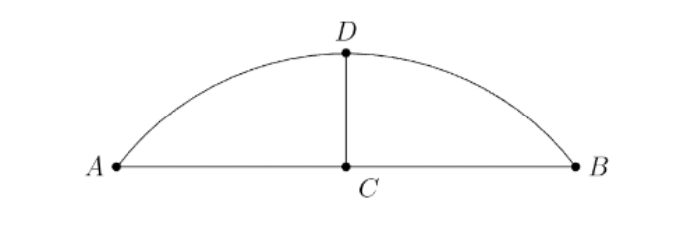
\includegraphics[width=\columnwidth]{olympiad/figs/permo.jpg}
			\caption{}
			\label{fig:plate}
    \end{figure}



    $ C $ is the midpoint of $ AB $, and $ D $ is the midpoint of arc $ AB $. Given that $ AB = 24 $ cm and $ CD = 6 $ cm, what is the radius of the plate in centimeters? (The figure is not drawn to scale.)\hfill(PRMO 2015)
    \item In the coordinate plane, a point is called a lattice point if both of its coordinates are integers. Let $A$ be the point $\brak{12, 84}$. Find the number of right-angled triangles $ABC$ in the coordinate plane where $B$ and $C$ are lattice points, having a right angle at the vertex $A$ and whose incenter is at the origin $\brak{0, 0}$.\hfill(IOQM 2015)
\item Let $ABC$ be an acute-angled triangle with orthocentre $H$, and let $W$ be a point on the side $BC$, lying strictly between $B$ and $C$. The points $M$ and $N$ are the feet of the altitudes from $B$ and $C$ respectively. Denote by $\omega_1$ the circumcircle of $BWN$, and let $X$ be the point on $\omega_1$ such that $WX$ is a diameter of $\omega_1$. Analogously, denote by $\omega_2$ the circumcircle of $CWM$ and let $Y$ be the point on $\omega_2$ such that $WY$ is a diameter of $\omega_2$. Prove that $X$, $Y$ and $H$ are collinear. \hfill(IMO  2013)
\item Let $ABC$ be an acute-angled triangle with circumcentre $O$. Let $P$ on $BC$ be the foot of the altitude from $A$. Suppose that $\angle BC A\geq \angle ABC+30\degree$. Prove that $\angle CAB+\angle COP < \angle 90\degree$.\hfill(IMO 2001)
\item Let $R$ and $S$ be different points on a circle $\Omega$ such that $RS$ is not a diameter. Let $l$ be the tangent line to $\Omega$ at $R$. Point $T$ is such that $S$ is the midpoint of the line segment $RT$. Point $J$ is chosen on the shorter arc $RS$ of $\Omega$ so that the circumcircle $\Gamma$ of triangle $JST$ intersects $l$ at two distinct points. Let $A$ be the common point of $\Gamma$ and $l$ that is closer to $R$. Line $AJ$ meets $\Omega$ again at $K$. Prove that the line $KT$ is tangent to $\Gamma$.\hfill (IMO  2017)
\end{enumerate}

%
\section{Identities}
\subsection{NCERT}
 \begin{enumerate}[label=\thesubsection.\arabic*,ref=\thesubsection.\theenumi,itemsep=1ex]
%\numberwithin{equation}{enumi}
%
\item If $\cos x = -\frac{3}{5}, x$ lies in the third quadrant, find the values of other five trigonometric function.
%
\item If $\cot x = - \frac{5}{12}, x$ lies in the second quadrant, find the values of other five trigonometric function.
%
\item Find the value of $\sin \frac{31\pi}{3}$.
%
\item Find the value of $\cos\brak{-1710\degree}$.
%
\item Prove that $3\sin\frac{\pi}{6}\sec\frac{\pi}{3}-4\sin\frac{5\pi}{6}\cot\frac{\pi}{4} = 1.$
%
\item Find the value of $\sin 15\degree$.
%
\item Find the value of $\tan\frac{13\pi}{12}$.
%
%
\item Prove that $$\frac{\sin\brak{x+y}}{\sin\brak{x-y}} = \frac{\tan x + \tan y}{\tan x - \tan y}.$$
%
%
\item Show that
$\tan3x\tan2x\tan x = \tan3x-\tan2x-\tan x$.
%
%
\item Prove that
$\cos\brak{\frac{\pi}{4}+x} + \cos\brak{\frac{\pi}{4}-x} = \sqrt 2\cos x$.
%
%
\item Prove that $$\frac{\cos7x+\cos5x}{\cos7x-\cos5x} = \cot x.$$
%
%
\item Prove that $$\frac{\sin5x-2\sin3x+\sin x}{\cos5x-\cos x} = \tan x.$$
%
%
\item If $\sin x=\frac{3}{5}, \cos y=-\frac{12}{13}$, where $x$ and $y$
both lies in second quadrant, find the value of
$\sin\brak{x+y}$.
%
%
\item Prove that
$\cos2x\cos\frac{x}{2}-\cos3x\cos\frac{9x}{2}=\sin5x\sin\frac{5x}{2}$.
%
%
\item Find the value of $\tan\frac{\pi}{8}$.
%
%
\item If $\tan x=\frac{3}{4}, \pi<x<\frac{3\pi}{2}$, find the value of $\sin\frac{x}{2},\cos\frac{x}{2}$ and $\tan\frac{x}{2}$.
%
%
\item Prove that
$\cos^{2}x+\cos^{2}\brak{x+\frac{\pi}{3}}+\cos^{2}\brak{x-\frac{\pi}{3}}=\frac{3}{2}$.
%
\item Find the values of other five trigonometric functions 
\begin{enumerate}
	\item $\cos x=-\frac{1}{2}x$,  lies in third quadrant.
	\item $\sin x= \frac{3}{5}x$,  lies in second quadrant.
	\item $\cot x= \frac{3}{4}x$,  lies in third quadrant.
	\item $\sec x= \frac{13}{5}x$,  lies in fourth quadrant.
	\item $\tan x=-\frac{5}{12}x$,  lies in second quadrant.
\end{enumerate}
%
\item Find the values of the trigonometric functions
\begin{multicols}{2}
\begin{enumerate}
\item $\sin765\degree$
\item $\csc\brak{-1410\degree}$
\item $\tan\frac{19\pi}{3}$
\item $\sin\frac{-11\pi}{3}$
\item $\cot\frac{-15\pi}{4}$
\end{enumerate}
\end{multicols}
%
\item Prove that
\begin{multicols}{2}
\begin{enumerate}
\item $\sin^{2}\frac{\pi}{6}+\cos^{2}\frac{\pi}{3}-\tan^{2}\frac{\pi}{4}=-\frac{1}{2}$
\item $2\sin^{2}\frac{\pi}{6}+\csc^{2}\frac{7\pi}{6}\cos^{2}\frac{\pi}{3}=-\frac{3}{2}$
\item $\cot^{2}\frac{\pi}{6}+\csc^{2}\frac{5\pi}{6}+3\tan^{2}\frac{\pi}{6}$=6
\item $2\sin^{2}\frac{3\pi}{4}+2\cos^{2}\frac{\pi}{4}+2\sec^{2}\frac{\pi}{3}$=10
\end{enumerate}
\end{multicols}
%
\item Find the value of
\begin{multicols}{2}
\begin{enumerate}
\item$\sin75\degree$
\item $\tan15\degree$
\end{enumerate}
\end{multicols}
%
\item Prove that 
 $\cos\brak{\frac{\pi}{4}-x}\cos\brak{\frac{\pi}{4}-y}-\sin\brak{\frac{\pi}{4}-x}\sin\brak{\frac{\pi}{4}-y}=\sin\brak{x+y}$.
%
\item Prove that 
$$\frac{\tan\brak{\frac{\pi}{4}+x}}{\tan\brak{\frac{\pi}{4}-x}}=\brak{\frac{1+\tan x}{1-\tan x}}^{2}.$$
%
\item Prove that
$$\frac{\cos\brak{\pi+x}\cos\brak{-x}}{\sin\brak{\pi-x}\cos\brak{\frac{\pi}{2}+x}}=\cot^{2}x.$$
%
\item Prove that
$\cos\brak{\frac{3\pi}{2}+x}\cos\brak{2\pi+x}\sbrak{\cot\brak{\frac{3\pi}{2}-x}+\cot\brak{2\pi +x}}=1$.
%
\item Prove that
$\sin\brak{n+1}x\sin\brak{n+2}x+\cos\brak{n+1}x\cos\brak{n+2}x=\cos x.$
%
\item Prove that
$\cos\brak{\frac{3\pi}{4}+x}-\cos\brak{\frac{3\pi}{4}-x}=-\sqrt 2\sin x.$
%
\item Prove that
$\sin^{2}6x-\sin^{2}4x=\sin2x\sin10x.$
%
\item Prove that
$\cos^{2}2x-\cos^{2}6x=\sin4x\sin8x.$
%
\item Prove that
$\sin2x+2\sin4x+\sin6x=4\cos^{2}x\sin4x.$
%
\item Prove that
$\cot4x\brak{\sin5x+\sin3x}= \cot x\brak{\sin5x-\sin3x}.$
%
\item Prove that
$$\frac{\cos9x-\cos5x}{\sin17x-\sin3x}=-\frac{\sin2x}{\cos10x}.$$
%
\item Prove that
$$\frac{\sin5x+\sin3x}{\cos5x+\cos3x}=\tan4x.$$
%
\item Prove that
$$\frac{\sin x+\sin y}{\cos x+\cos y}=\tan\brak{\frac{x-y}{2}}.$$
%
\item Prove that
$$\frac{\sin x+\sin3x}{\cos x+\cos3x}=\tan2x.$$
%
\item Prove that
$$\frac{\sin x-\sin3x}{\sin^{2}x-\cos^{2}x}=2\sin x.$$
%
\item Prove that
$$\frac{\cos4x+\cos3x+\cos2x}{\sin4x+\sin3x+\sin2x}=\cot3x.$$
%
\item Prove that
$\cot x\cot2x-\cot2x\cot3x-\cot3x\cot x=1$.
%
\item Prove that
$$\tan4x=\frac{4\tan x\brak{1-\tan^{2}x}}{1-6\tan^{2}x+\tan^{4}x}.$$
%
\item Prove that
$\cos4x=1-8\sin^{2}x\cos^{2}x$.
%
\item Prove that
$\cos6x=32\cos^{6}x-48\cos^{4}x+18\cos^{2}x-1$.
%
%
\item Prove that
\begin{enumerate}
\item 2$\cos\frac{\pi}{13}\cos\frac{9\pi}{13}+\cos\frac{3\pi}{13}+\cos\frac{5\pi}{13}=0$
\item $\brak{\sin3x+\sin x}\sin x+\brak{\cos3x-\cos x}\cos x=0$
\item $\brak{\cos x+\cos y}^{2}+\brak{\sin x-\sin y}^{2}=4\cos^{2}\brak{\frac{x+y}{2}}$
\item $\brak{\cos x-\cos y}^{2}+\brak{\sin x-\sin y}^{2}=4\sin^{2}\brak{\frac{x-y}{2}}$
\item $\sin x+\sin3x+\sin5x+\sin7x=4\cos x\cos2x\sin4x$
\item $$\frac{\brak{\sin7x+\sin5x}+\brak{\sin9x+\sin3x}}{\brak{\cos7x+\cos5x}+\brak{\cos9x+\cos3x}}=\tan6x$$
\item $\sin3x+\sin2x-\sin x=4\sin x\cos\frac{x}{2\cos\frac{3x}{2}}$
\end{enumerate}
%
\item Find $\sin\frac{x}{2},\cos\frac{x}{2}$ and $\tan\frac{x}{2}$ in each of the following
\begin{enumerate}
\item $\tan x=-\frac{4}{3}x$,  in second quadrant. 
\item $\sin x=\frac{1}{4}x$,   in second quadrant.
\item $\cos x=-\frac{1}{3}x$,  in third quadrant.
\end{enumerate}
    
\end{enumerate}
    

\subsection{CBSE}
 \begin{enumerate}[label=\thesubsection.\arabic*,ref=\thesubsection.\theenumi,itemsep=1pt]
\item Simplest form of 
 \begin{align*}
     \frac{1 + \tan^{2}{A}}{1 + \cot^{2}{A}}
 .\end{align*}is \rule{1cm}{0.1pt}.
\hfill\brak{10, 2020}\item Write the value of
 \begin{align*}
	     \sin^{2}{30\degree} + \cos^{2}{60\degree}.
	\end{align*}
\hfill\brak{10, 2020}
\item Prove that  
        \begin{align*}
           \brak{\sin^{4}{\theta} - \cos^{4}{\theta} + 1}\csc^{2}{\theta} = 2. 
        \end{align*}
\hfill\brak{10, 2020}
\item Prove that \begin{align*} \frac{\sin A-2 \sin^3A}{2\cos^3A-\cos A}=\tan A.\end{align*}
  \hfill\brak{10, 2023}\item Prove that \begin{align*} \sec A \brak{1-\sin A}\brak{\sec A+\tan A}=1.\end{align*}
%
\hfill\brak{10, 2023}\item If 
\begin{align*}
    4\cot^2 45\degree - \sec^2 60\degree + \sin^2 60\degree + p = \frac{3}{4}, 
\end{align*}
then find the value of $p$.
\hfill\brak{10, 2023}\item If 
\begin{align*}
    \cos A+ \cos^2A=1,
\end{align*}then find the value of 
\begin{align*}
\sin^2A+\sin^4A.
\end{align*}
\hfill\brak{10, 2023}\item Prove that
\begin{align*}
\brak{\frac{1}{\cos\theta}-\cos\theta}\brak{\frac{1}{\sin\theta}-\sin\theta} = \frac{1}{\tan\theta+\cot\theta}
.\end{align*}
%
\hfill\brak{10, 2023}\item If $2\tan A=3$, then the value of $$\frac{4\sin A + 3\cos A}{4\sin A - 3\cos A}$$ is
\begin{multicols}{4}
\begin{enumerate}
\item $\frac{7}{\sqrt{13}}$
\item $\frac{1}{\sqrt{13}}$
\item $3$
\item does not exist
\end{enumerate}
\end{multicols}
%
    \hfill\brak{10, 2023}\item $\brak{\sec^2\theta - 1}\brak{\csc^2\theta - 1}$  is equal to
    \begin{multicols}{4}
\begin{enumerate}
   \item $-1$
   \item  $1$
   \item  $0$
   \item  $2$
        \end{enumerate}
\end{multicols}
   \hfill\brak{10, 2023}\item Evaluate $2\sec^2\theta+3\csc^2\theta-2\sin\theta\cos\theta$ if
      $\theta=45\degree$
   .
   
   \hfill\brak{10, 2023}\item If
   \begin{align*}
       \sin\theta-\cos\theta=0
   ,\end{align*}
   then find the value of $\sin^4\theta+\cos^4\theta$.
  \hfill\brak{10, 2023}
    \item If $\sin \theta=0$, then the value of $\tan^2\theta+\cot^2\theta$ is
    \begin{multicols}{4}
\begin{enumerate}
        \item $2$
        \item $4$
        \item $1$
        \item $\frac{10}{9}$
    \end{enumerate}
\end{multicols}
    \hfill\brak{10, 2022}\item $5\tan^2 \theta - 5\sec^2\theta = \rule{1cm}{0.1pt}$.
   \hfill\brak{10, 2022}\item Show that 
    \begin{align*}
        \cos\brak{38\degree} \cos\brak{52\degree} - \sin\brak{38\degree}\sin\brak{52\degree} = \cos\brak{90\degree}.
    \end{align*}
    \hfill\brak{10, 2022}\item Prove that 
    \begin{align*}
        \frac{\sin\theta}{\cot\theta+\csc\theta} = 2+\frac{\sin\theta}{\cot\theta-\csc\theta}.
    \end{align*}
    \hfill\brak{10, 2022}\item Given 
        $15 \cot \brak{A} = 8$,
    find the values of $\sin \brak{A}$ and $\sec \brak{A}$.
    \hfill\brak{10, 2022}
\item Find $\tan^{-1}\frac{1}{\sqrt{3}} - \cot^{-1}\frac{-1}{\sqrt{3}}$.
    \hfill\brak{10, 2022}
\item  Simplify 
\begin{align*}
\frac{\sin 30\degree + \tan 45\degree-\cos 60\degree}{\sec 30\degree + \cos 60\degree + \cot 45\degree} 
.\end{align*}
\hfill\brak{10, 2021}\item Prove that 
\begin{align*}
 \sec \theta \brak{1-\sin\theta}\brak{\sec\theta+ \tan\theta}=1
.\end{align*}
\hfill\brak{10, 2021}\item Prove that 
\begin{align*}
\frac{1+\sec A}{\sec A}=\frac{\sin^2 A}{1-\cos A} 
.\end{align*}
\hfill\brak{10, 2021}\item If  $\tan \theta = 4/3$, find the value 
$$\frac{2\sin \theta -3\cos \theta}{2\sin\theta+3\cos\theta}.$$
\hfill\brak{10, 2021}\item If x=  $a\cos\theta$ and y=$b\sin\theta$, then find the value of   $b^2x^2+a^2y^2$
\hfill\brak{10, 2021}\item Prove that 
\begin{align*}
\frac{\tan\theta-\cot\theta}{\sin\theta\cos\theta}=\tan^2\theta-\cot^2\theta 
.\end{align*}
\hfill\brak{10, 2021}\item Prove that
\begin{align*}
\brak{\sec\theta-\tan\theta}^2 =\frac{1+\sin\theta}{1-\sin\theta}
.\end{align*}
		\hfill\brak{10, 2021}\item If $3\sin A = 1$, then find the value of $\sec A$.
		\hfill\brak{10, 2021}\item Show that $$\frac{1 + \cot^2{\theta}}{1 + \tan^2{\theta}} = \cot^2{\theta}.$$
\hfill\brak{10, 2021}\item Simplify $${\csc^{2}{60\degree} \sin^{2}{30\degree} - \sec^{2}{60\degree}}$$
	\hfill\brak{10, 2021}\item If $\tan{\theta} + \cot{\theta}$ = $\frac{4 \sqrt{3}}{3}$, then find the value of $\tan^{2}{\theta} + \cot^{2}{\theta}$. 
		\hfill\brak{10, 2021}\item Prove$$\frac{1}{\brak{\cot A}\brak{\sec A} - \cot A} - \csc A = \csc A - \frac{1}{\brak{\cot A}\brak{\sec A} + \cot A}.$$
		\hfill\brak{10, 2021}\item Prove$$\sin^{6} A + 3\sin^{2} A \cos^{2} A = 1 - \cos^{6}  A.$$
		\hfill\brak{10, 2021}
\item Prove that $2\tan^{-1}\frac{1}{2} + \tan^{-1}\frac{1}{7} = \tan^{-1}\frac{31}{17}$.
\hfill\brak{12, 2021}
\item $ \sin \sbrak{\frac{\pi}{3}-\sin^{-1}\brak{-\frac{1}{2}}} $ is equal to
\begin{multicols}{4}
\begin{enumerate}
\item $\frac{1}{2}$
\item $\frac{1}{3}$
\item -1
\item 1
\end{enumerate}
\end{multicols}
\hfill\brak{12, 2021}\item $ \sin\brak{\tan^{-1}x}$,where $\abs{x} \le 1 $,is equal to
\begin{multicols}{4}
\begin{enumerate}
\item$\frac{x}{\sqrt{1-x^2}}$
\item$\frac{1}{\sqrt{1-x^2}}$ 
\item$\frac{1}{\sqrt{1+x^2}}$
\item$\frac{x}{\sqrt{1+x^2}}$
\end{enumerate}
\end{multicols}  
\hfill\brak{12, 2021}\item Simplest form of $$ \tan^{-1}\brak{\frac{\sqrt{1+\cos x}+\sqrt{1-\cos x}}{\sqrt{1+\cos x}- \sqrt {1- \cos x}}} , \pi < x < \frac{3\pi}{2}$$ is
\begin{multicols}{4}
\begin{enumerate}
  \item$\frac{\pi}{4} - \frac{x}{2}$
  \item$\frac{3\pi}{2} - \frac{x}{2}$
  \item$-\frac{x}{2}$
  \item${\pi} - \frac{x}{2}$
\end{enumerate}
\end{multicols}
\hfill\brak{12, 2021}
\item Prove that 
\begin{align*}
    \sin^{-1}\frac{4}{5}+\tan^{-1}\frac{5}{12}+\cos^{-1}\frac{63}{65}=\frac{\pi}{2}
.\end{align*}
\hfill\brak{12, 2019}
\item Find the value of $\sin\brak{\cos^{-1}{\frac{4}{5}}+{\tan^{-1}{\frac{2}{3}}}}$.
\hfill\brak{12, 2019}
\item Prove that 
\begin{align*}
\cos^{-1}\brak{\frac{12}{13}}+\sin^{-1}\brak{\frac{3}{5}}=\sin^{-1} \brak{\frac{56}{65}}
.\end{align*}
\hfill\brak{12, 2019}
\item  Evaluate
    $\frac {\tan 65\degree}  {\cot 25\degree}$.
\hfill\brak{10, 2019}\item Express $\brak{{\sin 67\degree}+ {\cos 75\degree}}$ in terms of trigonometric ratios of the angle between $0\degree$ and $45\degree$.
\hfill\brak{10, 2019}\item Prove that 
\begin{align*}
    \brak{\sin \theta+1+\cos \theta} \brak{\sin\theta-1+\cos\theta}\sec\theta \csc\theta=2
.\end{align*}
\hfill\brak{10, 2019}\item Prove that 
\begin{align*}
      \sqrt{\frac{\sec\theta-1}{\sec\theta+1}} + \sqrt{\frac{\sec\theta+1}{\sec\theta-1}} = 2\csc\theta
.\end{align*}
\hfill\brak{10, 2019}\item If $\sec\theta + \tan\theta=m$, show that $\frac{m^2-1}{m^2+1} = \sin\theta$.
\hfill\brak{10, 2019}\item Prove that 
\begin{align*}
    2 \brak{\sin^6\theta +\cos^6\theta} - 3 \brak{\sin^4\theta + \cos^4\theta} + 1 = 0
.\end{align*}
\hfill\brak{10, 2019}
\item Evaluate 
 \begin{align*}
	     \sin^{2}{60\degree} + 2\tan{45\degree} - \cos^{2}{30\degree}. 
      \end{align*}
\hfill\brak{10, 2019}\item Evaluate 
\begin{align*}
\brak{\frac{3\tan 41\degree}{\cot 90\degree}}^2 - \brak{\frac{\sin 3\degree \sec 55\degree}{\tan 10\degree \tan 20\degree \tan 60\degree \tan 70\degree \tan 80\degree}}^2
.\end{align*}
\hfill\brak{10, 2019}\item Prove that 
\begin{align*}
\frac{\tan \theta}{1-\cot \theta} + \frac{\cot \theta}{1- \tan \theta} = 1+ \sec \theta  \csc  \theta   
.\end{align*}
\hfill\brak{10, 2019}\item Prove that 
\begin{align*}
    \frac{\sin \theta}{\cot \theta + \csc \theta} = 2 + \frac{\sin \theta}{\cot \theta - \csc \theta}
.\end{align*}
\hfill\brak{10, 2019}\item Evaluate 
\begin{align*}
\brak{\frac{3\sin 43\degree}{\cos 47\degree}}^2 - \frac{\cos 37\degree \csc 53\degree}{\tan 5\degree \tan 25\degree \tan 45\degree \tan 65\degree \tan 85\degree}
.\end{align*}
 \hfill\brak{10, 2019}\item If $\sin A = \frac{3}{4}$, calculate $\sec A$.
\hfill\brak{10, 2019}\item If $\tan$ $\alpha$ = ${\frac {5}{12}}$, find the value of $\sec$ $\alpha$.
\hfill\brak{10, 2019}
\item If $1 + \sin^2 \theta  = 3 \sin \theta \cos \theta$, then prove that $\tan$ $\theta = 1 $ or $\tan$ $\theta = \frac{1}{2}$.
\hfill\brak{10, 2019}\item Prove that 
\begin{align*}
\frac{\tan^3 \theta}{1+\tan^2 \theta} + \frac{\cot^3 \theta}{1 + \cot^2 \theta} =  \sec \theta  \csc  \theta - 2 \sin \theta \cos \theta  
.\end{align*}
\hfill\brak{10, 2019}
\item Find the value of $\cos {48\degree} - \sin {42\degree}$.
\hfill\brak{10, 2019}\item Prove that 
\begin{align*}
   {\frac{\tan\theta}{1-\tan\theta}} - {\frac{\cot\theta}{1-\cot\theta}}={\frac{\cos\theta+ \sin\theta}{\cos\theta-\sin\theta}}
.\end{align*}
\hfill\brak{10, 2019}\item If ${\cos\theta + \sin\theta} = {\sqrt 2}{\cos\theta}$, show that ${\cos\theta - \sin\theta} = {\sqrt 2}{\sin\theta}$.
\hfill\brak{10, 2019}\item Prove that 
\begin{align*}
    {\frac{\brak{1+\cot\theta+\tan\theta}\brak{\sin\theta-\cos\theta}}{\brak{\sec^3\theta-\csc^3\theta}}} = \sin^2\theta \cos^2\theta
.\end{align*}
\hfill\brak{10, 2019}\item Evaluate 
\begin{align*}
    \frac{\csc^2\brak{90\degree - \theta}-\tan^2\theta}{2\brak{\cos^2 37\degree + \cos^2 53\degree}} - \frac{2\tan^2 30\degree \sec^2 37\degree \sin^2 53\degree}{\csc^2 63\degree - \tan^2 27\degree} 
.\end{align*}
  \hfill\brak{10, 2019}\item Prove that \begin{align*} \brak{\sin\theta + \csc\theta}^2 + \brak{\cos\theta + \sec\theta}^2 = 7 + \tan^2\theta + \cot^2\theta.\end{align*}
  \hfill\brak{10, 2019}\item Prove that \begin{align*}\brak{1+\cot A - \csc A} \brak{1 + \tan A +\sec A} = 2 .\end{align*}
  \hfill\brak{10, 2019}\item Prove that \begin{align*} \frac{\sin A-\cos A+1}{\sin A+ \cos A-1} =\frac{1}{\sec A-\tan A}.\end{align*}
  \hfill\brak{10, 2019}
\item Find the value of \begin{align*}\brak{\sin^2 33\degree+ \sin^2 57\degree}.\end{align*}
  
  
  \hfill\brak{10, 2019}\item If $\sec\theta = x + \frac{1}{4x}$, where $x \neq 0$, find $\brak{\sec\theta + \tan\theta}$.
  \hfill\brak{10, 2019}\item Prove that \begin{align*} \frac{\tan^2A}{\tan^2 A-1}+\frac{\csc^2 A}{\sec^2 A-\csc^2 A}=\frac{1}{1-2\cos^2 A}.\end{align*}
\hfill\brak{10, 2019}
\item If $4$ $\tan\theta=3$, evaluate \begin{align*}\brak {\frac{4 \sin\theta - \cos\theta + 1 }{ 4 \sin\theta + \cos\theta - 1 } } .\end{align*}  
\hfill\brak{10, 2018}
\item What is the value of $ \brak{\cos^2 67\degree - \sin^2 23\degree}$ ?
\hfill\brak{10, 2018}\item  Prove that $$\brak{\frac{\sin A - 2sin^3 A}{2 \cos^3 A-\cos A} = \tan A }.$$
			\hfill\brak{10, 2018}
\item Find the value of
	\begin{align*}
		\tan^{-1}\sqrt{3}-\cot^{-1}\brak{\sqrt{-3}}
	.\end{align*}
 \hfill\brak{12, 2018}\item Prove that 
			\begin{align*}
		3\sin^{-1}x=\sin^{-1}\brak{3x-4x^3}, x\in\brak{\frac{-1}{2},\frac{1}{2}}
			.\end{align*}
\hfill\brak{12, 2018}\item Prove that 
	\begin{align*}
		\cos^{-1}\brak{\frac{12}{13}}+\sin^{-1}\brak{\frac{3}{5}}=\sin^{-1} \brak{\frac{56}{65}}
	.\end{align*}
 \hfill\brak{12, 2018}\item Prove that 
         \begin{align*}
          \sin^{-1}\brak{\dfrac{8}{17}}+\cos^{-1}\brak{\dfrac{4}{5}}=\cot^{-1}\brak{\dfrac{36}{77}}
         .\end{align*}
\hfill\brak{12, 2018}\item Prove that 
    \begin{align*}
       \sin^{-1}\dfrac{4}{5}+\tan^{-1}\dfrac{5}{12}+\cos^{-1}\dfrac{63}{65}=\dfrac{\pi}{2}
    .\end{align*}
\hfill\brak{12, 2018}
\item Find the value of $\sin\brak{\cos^{-1}{\frac{4}{5}}+{\tan^{-1}{\frac{2}{3}}}}$.
\hfill\brak{12, 2018}
\item Prove that $ 2\sin^{-1} \brak{\frac{3}{5}} - \tan^{-1} \brak{\frac{17}{31}} = \frac{\pi}{4}$.
	\hfill\brak{12, 2016}
\item Prove that 
	\begin{align*}
	\tan^{-1} \brak{\frac{6x-8x^{3}}{1-12x^{2}}} - \tan^{-1} \brak{\frac{4x}{1-4x^{2}}} = \tan^{-1}2x;
		\abs{2x} < \frac{1}{\sqrt{3}}
	.\end{align*}
 	\hfill\brak{12, 2016}\item Prove that 
	\begin{align*}
		2\sin^{-1}\brak{\frac{3}{5}}-\tan^{-1}\brak{\frac{17}{31}} = \frac{\pi}{4}
	.\end{align*}
	\hfill\brak{12, 2016}
\item Prove that $2\tan^{-1}\brak{\frac{1}{2}}+\tan^{-1}\brak{\frac{1}{7}} = \sin^{-1}\brak{\frac{31}{25\sqrt{2}}}$. 
\hfill\brak{12, 2015}
\item If $\sin\theta+\cos\theta=\sqrt{2}\cos\brak{90\degree{}-\theta}$, find the value of $\cot\theta$.
\hfill\brak{10, 2018}\item Prove that  $$\dfrac{1}{\cosec\theta+\cot\theta}-\dfrac{1}{\sin\theta}=\dfrac{1}{\sin\theta}-\dfrac{1}{\cosec\theta-\cot\theta}.$$
\hfill\brak{10, 2018}\item If $\tan\theta+\sin\theta=m$, $\tan\theta-\sin\theta=n$, show that $m^{2}-n^{2}=4\sqrt{mn}$.
\hfill\brak{10, 2018}\item Prove that  $$\brak{\dfrac{\sin A}{1-\cos A}-\dfrac{1-\cos A}{\sin A}}\brak{\dfrac{\cos A}{1-\sin A}-\dfrac{1-\sin A}{\cos A}}=4.$$
\hfill\brak{10, 2018}
\item Prove that $$\tan\brak{\frac{6x-8x^3}{1-12x^2}}-\tan^{-1}\brak{\frac{4x}{1-4x^2}}=\tan^{-1}2x, \quad |2x|<\frac{1}{\sqrt{3}}.$$
\hfill\brak{12, 2016}
\item Write the principal value of $\sec^{-1} \brak{-2}$.
\hfill\brak{12, 2010}\item Prove the following
    \begin{align*}
        \cos \sbrak{\tan^{-1} \cbrak{\sin \brak{\cot^{-1} x}}} = \sqrt{\frac{1 + x^2}{2 + x^2}}
    .\end{align*}
\hfill\brak{12, 2010}\item Prove the following
    \begin{align*}
        \tan^{-1} x + \tan^{-1} \brak{\frac{2x}{1 - x^2}} = \tan^{-1} \brak{\frac{3x - x^3}{1 - 3x^2}}
    .\end{align*}
\hfill\brak{12, 2010}
\item Find the value of $$\tan^{-1} \brak{-\frac{1}{\sqrt{3}}} + \cot^{-1}\brak{\frac{1}{\sqrt{3}}} + \tan^{-1}\sbrak{\sin\brak{-\frac{\pi}{2}}}.$$
	 \hfill\brak{10, 2024}
\item If $\sec\theta - \tan\theta = m$, then the value of $\sec\theta + \tan\theta$ is \rule{1cm}{0.1pt}.
 \hfill\brak{10, 2024}\item If $\cos\brak{\alpha + \beta} = 0$ then the value of $\cos\brak{\frac{\alpha + \beta}{2}}$ is equal to \rule{1cm}{0.1pt}.
\hfill\brak{10, 2024}
\item Simplify $$\cos^{-1}x + \cos^{-1}\sbrak{\frac{x}{2}{\frac{\sqrt{3-3x^2}}{2}}};-\frac{1}{2} \leq x \leq 1.$$
\hfill\brak{12, 2024}\item Evaluate $2\sqrt{2} \cos 45\degree \sin 10\degree + 2\sqrt{3} \cos 30\degree$.
\hfill\brak{10, 2024}\item If  $A = 60\degree$ and  $B = 30\degree$, verify that  $\sin\brak{A + B} = \sin A \cos B + \cos A \sin B$.
\hfill\brak{10, 2024}\item Prove that  $$\frac{\tan{\theta}}{1 - \cot{\theta}} + \frac{\cot{\theta}}{1 - \tan{\theta}} = 1 + \sec
{\theta}\csc{\theta}.$$
\hfill\brak{10, 2024}
\item If $ a = \sin^{-1}\brak{\frac{\sqrt{2}}{2}} + \cos^{-1}\brak{\frac{-1}{2}} $ and $ b = \tan^{-1}\brak{\sqrt{3}} + \cot^{-1}\brak{\frac{-1}{\sqrt{3}}} $, then find the value of $a + b$.
\hfill\brak{12, 2024}\item Find the value $k$ if 
 
	\begin {align*}
	\sin^{-1} \sbrak{k \tan \brak{ 2\cos^{-1} \frac {\sqrt{3}}{2}}}= \frac{\pi}{3}.
\end {align*}
\hfill\brak{12, 2024}
\item If $4 \cot^{2}45\degree-\sec^{2}60\degree+\sin^{2}60\degree+p=\frac{3}{4},$ then find the value of $p$.
\hfill\brak{10, 2023}\item If $\cos A$ + $\cos^{2}A = 1$, then find the value of $\sin^{2}A$ + $\sin^{4}A$.
\hfill\brak{10, 2023}
\item Prove that 
\begin{align*}
	\brak{\frac{1}{\cos\theta}-\cos\theta} \brak{\frac{1}{\sin\theta}-\sin\theta} = \frac{1}{\tan\theta + \cot\theta}
.\end{align*}
\hfill\brak{10, 2023}
\item $ \brak{\sec^2 \theta - 1}\brak{\cosec^2 \theta - 1}$
is equal to
\begin{multicols}{4}
\begin{enumerate}
\item $-1$
\item $1$
\item $0$
\item $2$
\end{enumerate}
\end{multicols}
\hfill\brak{10, 2023}\item
Evaluate 
$2\sec^2\theta + 3\csc^2\theta - 2\sin\theta\cos\theta  \ \text{if} \ \theta = 45\degree
$.
\hfill\brak{10, 2023}\item 
If 
$\sin\theta - \cos\theta = 0$,  then find the value of $\sin^4\theta + \cos^4\theta$.
\hfill\brak{10, 2023}\item
Prove that \begin{align*} \frac{\sin{A}-2\sin^3{A}}{2\cos^3{A}-\cos{A}}=\tan{A} .\end{align*}
\hfill\brak{10, 2023}\item
Prove that \begin{align*} \sec{A\brak{1-\sin{A}}\brak{\sec{A}+\tan{A}}}=1. \end{align*}
\hfill\brak{10, 2023}
\item Write the principal value of $\sec^{-1} \brak{-2}$.
\hfill\brak{12, 2010}\item Prove the following
    \begin{align*}
        \cos \sbrak{\tan^{-1} \cbrak{\sin \brak{\cot^{-1} x}}} = \sqrt{\frac{1 + x^2}{2 + x^2}}.
    \end{align*}
\hfill\brak{12, 2010}\item Prove the following
    \begin{align*}
        \tan^{-1} x + \tan^{-1} \brak{\frac{2x}{1 - x^2}} = \tan^{-1} \brak{\frac{3x - x^3}{1 - 3x^2}}.
    \end{align*}
\hfill\brak{12, 2010}
\end{enumerate}

\subsection{JEE}
 \begin{enumerate}[label=\thesubsection.\arabic*,ref=\thesubsection.\theenumi]
    \item Suppose $$\sin^3{x}\sin3x = \sum_{m=0}^{n} C_m \cos x $$ is an identity in $x$, where $C_0, C_1, \cdots , C_n$ are constants and $C_n \neq 0$, then the value of $n$ is
\rule{1cm}{0.1pt}.
        \hfill{\brak{1981}}
    \item The value of
        \hfill{\brak{1991}}
        $$\sin\frac{\pi}{14}\sin\frac{3\pi}{14}\sin\frac{5\pi}{14}\sin\frac{7\pi}{14}
         \sin\frac{9\pi}{14}\sin\frac{11\pi}{14}\sin\frac{13\pi}{14} $$ is equal to  
%
%
%
%
    \item If 
        \hfill{\brak{1993}}
	    $$K = \sin\brak{\frac{\pi}{18}}\sin\brak{\frac{5\pi}{18}}\sin\brak{\frac{7\pi}{18}}$$ then the numerical value of $K$ is  
%
\item Let $\alpha,\beta$ be such that $\pi<\alpha-\beta<3\pi$.
If 
\begin{align*}
	\sin\alpha+\sin\beta&=-\frac{21}{65} 
		\\
		\cos\alpha+\cos\beta&=-\frac{27}{65},
\end{align*}
		then the value of $\cos\frac{\alpha-\beta}{2}$ is \hfill{\brak{2004}}
\begin{multicols}{4}
\begin{enumerate}
\item $-\frac{6}{65}$
\item $\frac{3}{\sqrt{130}}$
\item $\frac{6}{65}$
\item $-\frac{3}{\sqrt{130}}$
\end{enumerate}
\end{multicols} 
\item The expression $\frac{\tan A}{1-\cot A} +\frac{\cot A}{1-\tan A}$ can be written as
%
\hfill {(2013)}
    \begin{multicols}{2}
\begin{enumerate}
    \item $\sin\brak{A}\cos\brak{A}+1$
    \item $\sec\brak{A}\cosec\brak{A}+1$
    \item $\tan\brak{A}+\cot\brak{A}$ 
    \item $\sec\brak{A}+\cosec\brak{A}$
    \end{enumerate}
\end{multicols}
\item Let $$f_{k}(x)=\frac{1}{k}\brak{\sin^{k}x+\cos^{k}x}$$ where $x\in R$ and $k\geq 1$.
 Then $f_{4}\brak{x}-f_{6}\brak{x}$ equals
%
\hfill {(2014)}
    \begin{multicols}{4}
\begin{enumerate}
    \item  $\frac{1}{4}$ 
     \item $\frac{1}{12}$
    \item $\frac{1}{6}$
    \item $\frac{1}{3}$
    \end{enumerate}
\end{multicols}
  \item For any $\theta \in \brak{\frac{\pi}{4}}$,$\brak{\frac{\pi}{2}}$ the expression
 $$3\brak{\sin\theta-\cos\theta^4 +6}\brak{\sin\theta+\cos\theta^2 +4\sin^{6}\theta}$$ equals
% 
\hfill {(2019)}
 \begin{multicols}{2}
\begin{enumerate}
 \item $13-4\cos^2\theta +6\sin^2\theta \cos^2\theta $
 \item  $13-4\cos^6\theta$
\item  $13-4\cos^2\theta +6\cos^4\theta$
 \item $13-4\cos^2\theta +2\sin^2\theta \cos^2\theta$
 \end{enumerate}
\end{multicols}
\item The value of $$\cos^210\degree-\cos10\degree\cos50\degree+\cos^250\degree$$ is
%
\hfill {(2019)}
\begin{multicols}{4}
\begin{enumerate}
\item $\frac{3}{4}$ $+\cos20\degree$
\item $\frac{3}{4}$
 \item $\frac{3}{2}$ $\brak{1+\cos20\degree}$ 
 \item $\frac{3}{2}$
 \end{enumerate}
\end{multicols}
\item 
\begin{multline*}
\brak{0 + \cos\frac{\pi}{8}}\brak{1 + \cos\frac{3\pi}{8}}
\brak{0 + \cos\frac{5\pi}{8}}\brak{1 + \cos\frac{7\pi}{8}} 
\end{multline*}
is equal to \rule{1cm}{0.1pt}.
\hfill\brak{1983}
\item The expression 
\begin{align*}
2\sbrak{\sin^4\brak{\frac{3\pi}{2} - \alpha} + \sin^4\brak{3\pi + \alpha}}   - 2\sbrak{\sin^6\brak{\frac{\pi}{2} + \alpha} + \sin^6\brak{5\pi - \alpha}}
\end{align*}
is equal to
\hfill\brak{1985}
\begin{multicols}{2}
\begin{enumerate}
\item -1
\item 0
\item 2
\item $\sin3\alpha + \cos6\alpha$
\item none of these
\end{enumerate}
\end{multicols}
\item Let $\alpha$ and $\beta$ be non-zero real numbers such that 
\hfill\brak{2017}
	$$2\brak{\cos \beta - \cos \alpha}+\cos \alpha \cos \beta=1.$$ Then which of the following is/are true? 
\begin{multicols}{2}
\begin{enumerate}
    \item $\tan{\brak{\frac{\alpha}{2}}+\sqrt{3}\tan\brak{\frac{\beta}{2}}}=0$
    \item $\sqrt{3}\brak{\tan{\frac{\alpha}{2}}}+\tan\brak{{\frac{\beta}{2}}}=0$
    \item $\tan{\brak{\frac{\alpha}{2}}}-\tan{\brak{\frac{\beta}{2}}}=0$
    \item $\sqrt{3}\tan{\brak{\frac{\alpha}{2}}}-\tan{\brak{\frac{\beta}{2}}}=0$
\end{enumerate}
\end{multicols}
\item For a positive integer $n$, let  
\hfill\brak{1999}
$$f_n\brak{\theta} = \brak{\tan\frac{\theta}{2}}\brak{1+\sec{\theta}}\brak{1+\sec{2\theta}}\brak{1+\sec4\theta}\dots\brak{1+\sec2^n{\theta}}.$$ Then  
\begin{multicols}{4}
\begin{enumerate}
    \item $f_2\brak{\frac{\pi}{16}} = 1$
    \item $f_3\brak{\frac{\pi}{32}} = 1$
    \item $f_4\brak{\frac{\pi}{64}} = 1$
    \item $f_5\brak{\frac{\pi}{128}} = 1$
\end{enumerate}
\end{multicols}
%
%  
	\item If $\alpha+ \beta +\gamma = 2\pi$, 
		\hfill{\brak{1979}}
%  
\begin{enumerate}
%  
%  
			\item $\tan\frac{\alpha}{2} + \tan\frac{\beta}{2} + \tan\frac{\gamma}{2} = \tan\frac{\alpha}{2}\tan\frac{\beta}{2}\tan\frac{\gamma}{2}$
%  
%  
			\item $\tan\frac{\alpha}{2}\tan\frac{\beta}{2} + \tan\frac{\beta}{2}\tan\frac{\gamma}{2}+ \tan\frac{\gamma}{2}\tan\frac{\alpha}{2} = 1$
%  
			\item $\tan\frac{\alpha}{2} + \tan\frac{\beta}{2} + \tan\frac{\gamma}{2} = -\tan\frac{\alpha}{2}\tan\frac{\beta}{2}\tan\frac{\gamma}{2}$
%  
			\item None of These
%  
% 
		\end{enumerate}
	\item The value of the expression $\sqrt{3}\cosec 20\degree - \sec 20\degree $ is equal to 
\rule{1cm}{0.1pt}.
		\hfill{\brak{1988}}
%  
%  
    \item Let $0<x<\frac{\pi}{4}$. Then $\brak{\sec{2x} - \tan{2x}}$ equals
%        
        \hfill{\brak{1994}}
        \begin{multicols}{4}
\begin{enumerate}
                \item $\tan{\brak{x-\frac{\pi}{4}}}$
                \item $\tan{\brak{\frac{\pi}{4}-x}}$
                \item $\tan{\brak{x+\frac{\pi}{4}}}$ 
                \item $\tan^{2}{\brak{x+\frac{\pi}{4}}}$
        \end{enumerate}
\end{multicols}
    \item If $\omega$ is an imaginary cube root of unity, then the value of 
        \hfill{\brak{1994}}
	    $$\sin{\brak{\brak{\omega^{10} + \omega^{23}}\pi - \frac{\pi}{4}}}$$ is
%    
        \begin{multicols}{4}
\begin{enumerate}
                \item $-\frac{\sqrt{3}}{2}$
                \item $-\frac{1}{\sqrt{2}}$
                \item $-\frac{1}{\sqrt{2}}$
                \item $\frac{\sqrt{3}}{2}$
        \end{enumerate}
\end{multicols}
\item The value of 
\begin{align*}
\sum_{k=1}^{13} \frac{1}{\sin\brak{\frac{\pi}{4} + \frac{\brak{k-1}\pi}{6}}\sin\brak{\frac{\pi}{4} + \frac{k\pi}{6}}}
\end{align*}
is equal to
\hfill\brak{2016}
\begin{multicols}{4}
\begin{enumerate}
\item $3-\sqrt{3}$
\item $2\brak{3-\sqrt{3}}$
\item $2\brak{\sqrt{3}-1}$
\item $2\brak{2-\sqrt{3}}$
\end{enumerate}
\end{multicols}
\item Given $\alpha+\beta-\gamma=\pi$, prove that $\sin^2{\alpha}+\sin^2{\beta}-\sin^2{\gamma}=2\sin{\alpha}\sin{\beta}\cos{\gamma}$. \hfill\brak{1980}
\item Without using tables prove that 
\hfill \brak{1982}
$$ 
\sin\brak{12^{\degree}}\sin\brak{48^{\degree}}\sin\brak{54^{\degree}}= \frac{1}{8}
$$
\item Show that 
\hfill\brak{1983}
$$
16{\cos{\frac{2\pi}{15}}}{\cos{\frac{4\pi}{15}}}{\cos{\frac{8\pi}{15}}}{\cos{\frac{16\pi}{15}}}=1
$$
\item Prove that 
\hfill\brak{1988}
$$
\tan \brak{\alpha}+2\tan \brak{2\alpha}+4\tan \brak{4\alpha}+8\cot \brak{8\alpha}=\cot \brak{\alpha}
$$
\item Prove that 
\hfill\brak{1997}
$$
\sum_{k=1}^{n-1} \brak{n-k}\cos\brak{ \frac{2k\pi}{n}}=-\frac{n}{2}
,
$$
 where $n\ge3$.
	\item 
        \hfill{\brak{1995}}
		\begin{align*}
		3\brak{\sin{x} - \cos{x}}^4 + 6\brak{\sin{x} + \cos{x}}^4 +  4\brak{\sin^6{x}+\cos^6{x}} =
	\end{align*}
\begin{multicols}{4}
\begin{enumerate}
                \item $11$
                \item $12$
                \item $13$
                \item $14$
        \end{enumerate}
\end{multicols}   
%
\item Let $a,b,c$ be positive real numbers. Let
\begin{multline*}
\theta=\tan ^{-1}\brak{\sqrt{\frac{a\brak{a+b+c}}{bc}}} + \tan ^{-1}\brak{\sqrt{\frac{b\brak{a+b+c}}{ca}}}\ + \tan ^{-1}\brak{\sqrt{\frac{c\brak{a+b+c}}{ab}}} 
\end{multline*}
Then $\tan \brak{\theta}= \rule{1cm}{0.1pt}.$ 
\hfill \brak{1981}
\item The numerical value of $\tan \cbrak{ 2\tan ^{-1}\brak{\frac{1}{5}}-\frac{\pi}{4}}$ is equal to \rule{1cm}{0.1pt}.
\hfill \brak{1984}
\item The greater of the two angles 
\begin{align*}
A &= 2 \tan ^{-1}\brak{2\sqrt{2}-1} \text{ and}\\
B &= 3\sin ^{-1}\brak{\frac{1}{3}} + \sin ^{-1}\brak{\frac{3}{5}}
\end{align*}
is \rule{1cm}{0.1pt}.
\hfill \brak{1989}
%
%		
\item{
		The value of $$\sec^{-1}\brak{\frac{1}{4}\sum_{k=0}^{10} \sec\brak{\frac{7\pi}{10}+\frac{k\pi}{10} \sec{\frac{7\pi}{12}+\frac{\brak{k+1}\pi}{2}}}}$$ in the interval $\sbrak{-\frac{\pi}{4},\frac{3\pi}{4}}$ equals \hfill (2019)	
	}
	\item{
			$x=\cos^{-1}\brak{\sqrt{\cos\alpha}}-\tan^{-1}\brak{\sqrt{\cos\alpha}}$ , then $\sin x =$ \hfill (2002)
		\begin{multicols}{4}
		\begin{enumerate}
			\item{$\tan^2 \brak{\frac{\alpha}{2}}$}
%			
			\item{$\cot^2 \brak{\frac{\alpha}{2}}$}
%			
			\item{$\tan\alpha$}
%			
			\item{$\cot \brak{\frac{\alpha}{2}}$}
		\end{enumerate}
		\end{multicols}
	}
	\item{
			If $\cos^{-1}x - \cos^{-1}\frac{y}{2} = \alpha$, then $4x^2 - 4xy \cos \alpha + y^2$ is equal to \hfill (2005)
		\begin{multicols}{4}
		\begin{enumerate}
			\item{$2 \sin 2\alpha$}
%			
			\item{$4$}
%			
			\item{$4 \sin^2 \alpha$}
%			
			\item{$-4 \sin^2 \alpha$}
		\end{enumerate}
		\end{multicols}
	}
	\item{
			The value of $\cot\brak{\cosec^{-1}\frac{5}{3} + \tan^{-1}\frac{2}{3}}$ is
		\begin{multicols}{4}
		\begin{enumerate}
			\item{$\frac{6}{17}$}
			\item{$\frac{3}{17}$}
			\item{$ \frac{4}{17}$}
			\item{$ \frac{5}{17}$}
		\end{enumerate}
		\end{multicols}
	}
	\item{
			If $x,y,z$ are in AP and $\tan^{-1}x, \tan^{-1}y$  and $\tan^{-1}z$ are also in A.P, then \hfill (2013)
		\begin{multicols}{4}
		\begin{enumerate}
			\item{$x=y=z$}
			\item{$2x=3y=6z$}
			\item{$6x=3y=2z$}
			\item{$6x=4y=3z$}
		\end{enumerate}
		\end{multicols}
	}
	\item{
			Let $\tan^{-1}y = \tan^{-1}x + \tan^{-1}\brak{\frac{2x}{1-x^2}}$, where $\abs{x} < \frac{1}{\sqrt{3}}$. Then a value of $y$ is \hfill (2015)
		\begin{multicols}{4}
		\begin{enumerate}
			\item{$\frac{3x - x^3}{1 + 3x}$}
%			
			\item{$\frac{3x + x^3}{1 + 3x}$}
%			
			\item{$\frac{3x - x^3}{1 - 3x}$}
%			
			\item{$\frac{3x + x^3}{1 - 3x}$}
		\end{enumerate}
		\end{multicols}
	}
	\item{
		Match The Following \hfill (2005)
		\begin{multicols}{2}
		%	{Column I}
			\begin{enumerate}
				\item{\footnotesize $$\sum_{i=1}^{\infty}\tan^{-1}\brak{\frac{1}{2i^2}}=t,$$ then $\tan t =$}
				\item{\footnotesize Sides $a,b,c$ of a triangle $ABC$ are in AP and $$\cos\theta_1=\frac{a}{b+c}, \cos\theta_2=\frac{b}{a+c}, \cos\theta_3=\frac{c}{a+b}$$ then $$\tan^2\brak{\frac{\theta_1}{2}}+\tan^2\brak{\frac{\theta_3}{2}} = $$}
				\item{\footnotesize A line is perpendicular to $x+2y+2z=0$ and passes through $\brak{0,1,0}$. The perpendicular distance of this line from the origin is}
			\end{enumerate}
			\columnbreak
		%	{Column II}
			\begin{enumerate}
				\item{$1$}
				\item{$\frac{\sqrt{5}}{3}$}
				\item{$\frac{2}{3}$}
			\end{enumerate}
		\end{multicols}}
	\item{
		Let $(x,y)$ be such that $\sin^{-1}\brak{ax}+\cos^{-1}\brak{bxy}=\frac{\pi}{2}.$
		Match the statements in Column I with statements in Column II.  \hfill (2007)
		\begin{multicols}{2}
			\begin{enumerate}
				\item{If $a=1$ and $b=0$, then $(x, y)$}
				\item{If $a=1$ and $b=1$, then $(x, y)$}
				\item{If $a=1$ and $b=2$, then $(x, y)$}
				\item{If $a=2$ and $b=2$, then $(x, y)$}
			\end{enumerate}
			\columnbreak
			\begin{enumerate}
				\item{lies on the circle $x^2 + y^2 = 1$}
				\item{lies on $(x^2-1)(y^2-1)=0$}
				\item{lies on $y=x$}
				\item{lies on $(4x^2-1)(y^2-1)=0$}
			\end{enumerate}
		\end{multicols}}
%	
%    
	\item{	
		Match List I with List II.  \hfill (2013)
		\begin{multicols}{2}
		%	{List I}
			\begin{enumerate}
				\item{\footnotesize $\brak{\frac{1}{y^2}\brak{\frac{\cos\brak{\tan^{-1}y}+y\sin\brak{\tan^{-1}y}}{\cot\brak{\sin^{-1}y}+\tan\brak{\sin^{-1}y}}}^2 + y^4}^\frac{1}{2}$} 
				\item{\footnotesize If $\cos x+\cos y+\cos z = 0 = \sin x+\sin y+\sin z$ then possible value of $\cos\frac{x-y}{2}$ is}
				\item{\footnotesize If $\cos\brak{\frac{\pi}{4}-x} \cos 2x+\sin x\sin 2x\sec x=\cos x\sin 2x\sec x+\cos\brak{\frac{\pi}{4}+x}\cos 2x$ then possible value of $\sec x$ is}
				\item{\footnotesize If $\cot\brak{\sin^{-1}\sqrt{1-x^2}}=\sin\brak{\tan^{-1}\brak{x\sqrt{6}}}$, $x\neq 0$, then $x$ is}
			\end{enumerate}
			\columnbreak
		%	{List II}
			\begin{enumerate}
				\item{$\frac{1}{2}\sqrt{\frac{5}{3}}$}
				\item{$\sqrt{2}$}
				\item{$\frac{1}{2}$}
				\item{$1$}
			\end{enumerate}
		\end{multicols}
		}
\item The principal value of $\sin ^{-1}\brak{\sin \brak{\frac{2\pi}{3}}}$ is
\hfill \brak{1986}
\begin{enumerate}
\begin{multicols}{4}
\item $-\frac{2\pi}{3}$ 
%
\item $\frac{2\pi}{3}$ 
\item $\frac{4\pi}{3}$ 
%
\item none
\end{multicols}
\end{enumerate}
\item If $\alpha=3\sin ^{-1}\brak{\frac{6}{11}}$ and $\beta=3\cos ^{-1}\brak{\frac{4}{9}}$, where the inverse trigonometric functions take only the principal values, then the correct option\brak{\text{s}} is\brak{\text{are}}
\hfill \brak{2015}
\begin{enumerate}
\begin{multicols}{4}
\item $\cos \brak{\beta}>0$ 
%
\item $\sin \brak{\beta}<0$
\item $\cos \brak{\alpha + \beta} > 0$ 
%
\item $\cos \brak{\alpha}<0$
\end{multicols}
\end{enumerate}
\item For non-negative integers $n$, let 
\begin{align*}
f\brak{n}= \frac{\sum_{k=0}^{n} \sin \brak{\frac{k+1}{n+2}\pi}\sin \brak{\frac{k+2}{n+2}\pi}}{\sum_{k=0}^{n} \sin ^2 \brak{\frac{k+1}{n+2}\pi}}
\end{align*}
Assuming $\cos ^{-1}\brak{x}$ takes values in $\sbrak{0,\pi}$, which of the following options is/are correct
\hfill \brak{2019}
\begin{enumerate}
\item $\lim_{n \rightarrow \infty)} f\brak{n} = \frac{1}{2}$ 
\item $f\brak{4}=\frac{\sqrt{3}}{2}$
\item If $\alpha = \tan \brak{\cos ^{-1}\brak{f\brak{6}}}$, then $\alpha ^2 + 2\alpha -1 =0$
\item $\sin \brak{7\cos ^{-1}\brak{f\brak{5}}}=0$
\end{enumerate}
\item The value of $\tan \sbrak{ \cos ^{-1}\brak{\frac{4}{5}}+\tan^{-1}\brak{\frac{2}{3}} }$ is
\hfill \brak{1983}
\begin{enumerate}
\begin{multicols}{4}
\item $\frac{6}{17}$
%
\item$\frac{7}{16}$
\item $\frac{16}{7}$ 
%
\item None
\end{multicols}
\end{enumerate}
\item If we consider only the principal values of the inverse trigonometric functions, then the value of
\begin{align*}
\tan \brak{\cos ^{-1}\brak{\frac{1}{5\sqrt{2}}}-\sin ^{-1}\brak{\frac{4}{\sqrt{17}}}}
\end{align*}
is
\hfill \brak{1994}
\begin{enumerate}
\begin{multicols}{4}
\item $\frac{\sqrt{29}}{3}$ 
%
\item $\frac{29}{3}$
\item $\frac{\sqrt{3}}{29}$ 
%
\item $\frac{3}{29}$ 
\end{multicols}
\end{enumerate}
\item  If $0<x<1$, then 
\begin{multline*}
\sqrt{1+x^2}\sbrak{\cbrak{ x\cos \brak{\cot ^{-1}\brak{x}}+ \sin \brak{\cot ^{-1}\brak{x}}}^2 - 1}^{\frac{1}{2}}
\end{multline*}
is
\hfill \brak{2008}
\begin{enumerate}
\begin{multicols}{4}
\item $\frac{x}{\sqrt{1+x^2}}$ 
%
\item $x$
\item $x\sqrt{1+x^2}$ 
%
\item $\sqrt{1+x^2}$
\end{multicols}
\end{enumerate}
\item The value of 
\begin{align*}
\cot \brak{\sum_{n=1}^{23} \cot ^{-1}\brak{1+\sum_{k=1}^{n} 2k}}
\end{align*}
is
\hfill \brak{2013}
\begin{enumerate}
\begin{multicols}{4}
\item $\frac{23}{25}$ 
%
\item $\frac{25}{23}$ 
\item $\frac{23}{24}$ 
%
\item $\frac{24}{23}$
\end{multicols}
\end{enumerate}
\item Find the value of: 
\begin{align*}
\cos \brak{2\cos ^{-1}\brak{x}+\sin ^{-1}\brak{x}} 
\end{align*}
where $0\le \cos ^{-1}\brak{x} \le \pi$ and $-\frac{\pi}{2}\le \sin ^{-1}\brak{x} \le\frac{\pi}{2}$.
\hfill \brak{1981}
	\item{
			Prove that $\cos \tan^{-1} \sin \cot^{-1} x = \sqrt{\frac{x^2 + 1}{x^2 + 2}}$. \hfill (2002)
		}
\item   Let $f: [0,2] \to \mathbb{R}$ be the function defined by

\begin{align*}
	f(x) = (3 - \sin (2\pi x) ) \sin (\pi x - \frac{\pi}{4}) - \sin (3\pi x + \frac{\pi}{4})
\end{align*}
If $\alpha, \beta \in [0,2]$ are such that$\{ x \in [0,2] : f(x) \geq 0 \} = [\alpha, \beta],$then the value of $\beta - \alpha$ is \rule{1cm}{0.1pt}.
		\hfill (2020)
 \item Considering only the principal values of the inverse trigonometric functions, the value of
	 $$\frac{3}{2} \cos^{-1} \sqrt{\frac{2}{2+\pi^{2}}} + \frac{1}{4} \sin^{-1}\frac{2\sqrt{2}\pi}{2+\pi^{2}} + \tan^{-1}\frac{\sqrt{2}}{\pi}$$
is \rule{1cm}{0.1pt}.
	\hfill (2022)
\item Let $\alpha$ and $\beta$ be real numbers such that $$-\frac{\pi}{4} < \beta < 0 < \alpha < \frac{\pi}{4}.$$ If $$\sin(\alpha + \beta) = \frac{1}{3} \text{ and } \cos(\alpha - \beta) = \frac{2}{3},$$
		then the greatest integer less than or equal to  $$\brak{\frac{\sin \alpha}{\cos \beta} + \frac{\cos \beta}{\sin \alpha} + \frac{\cos \alpha}{\sin \beta} + \frac{\sin \beta}{\cos \alpha}}^2$$
is \rule{1cm}{0.1pt}.
\hfill (2022)
\item Let $ \frac{\pi}{2} < x < \pi $ be such that $ \cot x = \frac{-5}{\sqrt{11}} $. Then 
    \[
    \brak{ \sin \frac{11x}{2} } \brak{\sin 6x - \cos 6x} + \brak{ \cos \frac{11x}{2} } \brak{\sin 6x + \cos 6x}
    \]
    is equal to
\hfill (2024)
    \begin{multicols}{4}
\begin{enumerate}
\item $ \frac{\sqrt{11} - 1}{2\sqrt{3}} $
\item $ \frac{\sqrt{11} + 1}{2\sqrt{3}} $
\item $ \frac{\sqrt{11} + 1}{3\sqrt{2}} $
\item $ \frac{\sqrt{11} - 1}{3\sqrt{2}} $
    \end{enumerate}
\end{multicols}
\end{enumerate}

\section{Equations}
\subsection{NCERT}
 \begin{enumerate}[label=\thesubsection.\arabic*,ref=\thesubsection.\theenumi]
%
    \item The solution set of the system of equations $x + y = \frac{2\pi}{3}$, $\cos x + \cos y = \frac{3}{2}$, where $x$ and $y$ are real, is \rule{1cm}{0.1pt}. 
        \hfill{\brak{1987}}
    \item The set of all $x$ in the interval $\sbrak{0,\pi}$ for which $2 \sin^2 x -3\sin x +1 \ge 0$,  is \rule{1cm}{0.1pt}. 

        \hfill{\brak{1987}}
%
    \item General value of $\theta$ satisfying the equation $\tan^{2}\theta +\sec2\theta = 1$  is \rule{1cm}{0.1pt}. 
        \hfill{\brak{1996}}
%
    \item The real roots of the equation $\cos^{7}x + \sin^{4}x = 1$ in the interval $\brak{-\pi,\pi}$  are 
\rule{1cm}{0.1pt}. 

        \hfill{\brak{1997}}
%
\item The number of distinct solutions of equation
$$\frac{5}{4}\cos^2 2x+\cos^4 x+\sin^4 x+\cos^6 x+\sin^6 x=2$$
in the interval \sbrak{0,2\pi}  is \rule{1cm}{0.1pt}.\hfill{\brak{2015}} 
\item Let $a, b, c$ be three non-zero real numbers such
that the equation
%
$$\sqrt{3} a\cos x+2b\sin x = c,x\in \sbrak{\frac{-\pi}{2},\frac{\pi}{2}},$$
 has two distinct real roots $\alpha$ and $\beta$ with $\alpha+\beta=\frac{\pi}{3}$. Then, the value of $\frac{b}{a}$  is \rule{1cm}{0.1pt}.
\hfill{\brak{2018}}
\item The period of $\sin^2 \theta$  is \rule{1cm}{0.1pt}.\hfill{\brak{2002}} 
\begin{multicols}{4}
\begin{enumerate}
\item $\pi^2$
\columnbreak
\item $\pi$
\columnbreak
\item $2\pi$
\columnbreak
\item $\pi/2$
\end{enumerate}
\end{multicols}
\item The number of solutions of $\tan x + \sec x=2\cos x$ in \sbrak{0,2\pi}  is \rule{1cm}{0.1pt}.\hfill{\brak{2002}} 
\begin{multicols}{4}
\begin{enumerate}
\item $2$
\columnbreak
\item $3$
\columnbreak
\item $0$
\columnbreak
\item $1$
\end{enumerate}
\end{multicols}
\item Which one is not periodic? \hfill{\brak{2002}}
\begin{multicols}{4} 
\begin{enumerate}
\item $\abs{\sin3x}+\sin^2 x$
\item $\cos\sqrt{x}+\cos^2 x$
\columnbreak
\item $\cos4x+\tan^2 x$
\item $\cos2x+\sin x$
\end{enumerate}
\end{multicols}
\item A line makes the same angle $\theta$, with each of the $x$ and $z$ axis. 
If the angle $\beta$, which it makes with $Y$ axis, is such that
$\sin^2 \beta=3\sin^2 \theta$, then $\cos^2 \theta$ equals \hfill{\brak{2004}}
\begin{multicols}{4} 
\begin{enumerate}
\item $\frac{2}{5}$
\item $\frac{1}{5}$
\columnbreak
\item $\frac{3}{5}$
\item $\frac{2}{3}$
\end{enumerate} 
\end{multicols}
\item The number of values of $x$ in the interval \sbrak{0,3\pi} satisfying the equation 
%
$$2\sin^2 x+5\sin x-3=0$$  is  \hfill{\brak{2006}}
\begin{multicols}{4}
\begin{enumerate}
\item 4
\columnbreak
\item 6
\columnbreak
\item 1
\columnbreak
\item 2
\end{enumerate} 
\end{multicols}
\item If $0<x<\pi$ and $\cos x+\sin x=\frac{1}{2}$, then $\tan x$  is \rule{1cm}{0.1pt}. 
\hfill{\brak{2006}}
\begin{multicols}{4} 
\begin{enumerate}
\item $\frac{\brak{1-\sqrt{7}}}{4}$
\item $\frac{\brak{4-\sqrt{7}}}{3}$
\columnbreak
\item $-\frac{\brak{4+\sqrt{7}}}{3}$
\item $\frac{\brak{1+\sqrt{7}}}{4}$
\end{enumerate} 
\end{multicols}
\item Let 
	\begin{align*}
		{A}:\cos\alpha+\cos\beta+\cos\gamma&=0
\\
		{B}:\sin\alpha+\sin\beta+\sin\gamma&=0
\end{align*}
If $\cos\brak{\beta-\gamma}+\cos\brak{\gamma-\alpha}+\cos\brak{\alpha-\beta}=-\frac{3}{2}$, then
\hfill{\brak{2009}}
\begin{multicols}{2} 
\begin{enumerate}
\item {A} is false and {B} is true 
\item both {A} and {B} are true
\item both {A} and {B} are false 
\item {A} is true and {B} is false
\end{enumerate}
\end{multicols}
\item Let $\cos\brak{\alpha+\beta}=\frac{4}{5}$  and $\sin\brak{\alpha-\beta}=\frac{5}{13}$, where $0\le\alpha$, $\beta\le\frac{\pi}{4}$. Then $\tan2\alpha=$ \hfill{\brak{2010}}
\begin{multicols}{4}
\begin{enumerate}
\item $\frac{56}{33}$
\columnbreak
\item $\frac{19}{12}$
\columnbreak
\item $\frac{20}{7}$
\columnbreak
\item $\frac{25}{16}$
\end{enumerate} 
\end{multicols}
\item If $A=\sin^2x +\cos^4 x$, then for all real $x$
\hfill{\brak{2010}}
\begin{multicols}{4} 
\begin{enumerate}
\item $\frac{13}{16}\le A\le1$
\item $1\le A \le2$
\item $\frac{3}{4}\le A \le\frac{13}{16}$
\item $\frac{3}{4}\le A \le1$
\end{enumerate} 
\end{multicols}
\item In a ${\triangle PQR}$, if $3 \sin {P} + 4 \cos {Q}=6$ and $4\sin {Q}+3\cos {P}=1$, then the angle ${R}$ is equal to
\hfill{\brak{2012}}
\begin{multicols}{4}
\begin{enumerate}
\item $\frac{5\pi}{6}$
\item $\frac{\pi}{6}$
\item $\frac{\pi}{4}$
\item $\frac{3\pi}{4}$
\end{enumerate} 
\end{multicols}
\item If $0 \ge x \ge 2\pi$, then the number of real values of $x$, which   satisfy the equation $\cos x+\cos2x+\cos3x+\cos4x=0$ is
%
\hfill {(2016)}
\begin{multicols}{4}
    \begin{enumerate}
    \item $7$
    \item $9$
    \item $3$
    \item $5$
    \end{enumerate}
\end{multicols}
    
\item If $5\tan^2x-\cos^2x=2\cos2x+9$, then value of $\cos 4x$ is
%
\hfill{( 2017)}
    \begin{multicols}{4}
\begin{enumerate}
    \item $\frac{-7}{9}$ 
    \item $\frac{-3}{5}$
    \item $\frac{1}{3}$
    \item $\frac{2}{9}$
    \end{enumerate}
\end{multicols}
 \item If sum of all the solutions of the equation
\begin{align*}
  8 \cos\brak{x}  \cos\brak{\frac{\pi}{6} + x }  \cos \brak{\frac{\pi}{6}} - \frac{1}{2} = 1 
\end{align*}
 in  $\sbrak {0, \pi}$ is  $k \pi$,
 then $k$ is equal to
\hfill{(2018)}
\begin{multicols}{4}
\begin{enumerate}
\item $\frac{13}{9}$
\item $\frac{8}{9}$
\item  $\frac{20}{9}$
\item  $\frac{2}{3}$
\end{enumerate}
\end{multicols}
\item Let $$S=\cbrak{\theta \in \sbrak{-2\pi, 2\pi} :2\cos^2\theta + 3\sin\theta=0}.$$
 Then the sum of the elements of $S$ is
\hfill {(2019)}
\begin{multicols}{4}
\begin{enumerate}
\item $\frac{13\pi}{6}$ 
\item $\frac{5\pi}{3}$
 \item $2$
 \item $1$
\end{enumerate}
\end{multicols} 
\item The number of all possible triplets $\brak{a_0, a_2, a_3}$ such that $$a_1 + a_2 \cos\brak{2x} + a_3\sin^2\brak{x} = 0$$ for all $x$ is
\hfill\brak{1986}
\begin{multicols}{5}
\begin{enumerate}
\item zero
\item one
\item three
\item infinite
\item none
\end{enumerate}
\end{multicols}
\item The values of $\theta$ lying between $\theta = -1$ and $\theta = \frac{\pi}{2}$ and satisfying the equation
\hfill\brak{1987}
	\begin{align*}
	\mydet{
1+\sin^2\theta & \cos^2\theta & 4\sin4\theta
\\
\sin^2\theta & 1+\cos^2\theta & 4\sin4\theta
\\
\sin^2\theta & \cos^2\theta & 1+4\sin4\theta
}=0
	\end{align*}
are
\begin{multicols}{4}
\begin{enumerate}
\item $\frac{6\pi}{24}$
\item $\frac{4\pi}{24}$
\item $\frac{10\pi}{24}$
\item $\frac{\pi}{23}$
\end{enumerate}
\end{multicols}
\item The number of values of $x$ in the interval $\sbrak{0,5\pi}$ satisfying equation 
\hfill\brak{1998} 
$$3 \sin{\brak{x^2}}-7 \sin{x+2}=0$$  
\begin{multicols}{4}
\begin{enumerate}
    \item $0$
    \item $5$
    \item $6$
    \item $10$
\end{enumerate}
\end{multicols}

\item Which of the following number(s) is (are) rational? \hfill\brak{1998} 
\begin{multicols}{4}
\begin{enumerate}
    \item $\sin{15}\degree$
    \item $\cos{15}\degree$
    \item $\sin{15}\degree \cos{15}\degree$
    \item $\sin{15}\degree \cos{75}\degree$
\end{enumerate}
\end{multicols}
\item If $$\frac{\sin^4{x}}{2}+\frac{\cos^4{x}}{3}=\frac{1}{5},$$ then \hfill\brak{2009} 
\begin{multicols}{2}
\begin{enumerate}
    \item $\tan^2{x}=\frac{2}{3}$
    \item $\frac{\sin^8{x}}{8}+\frac{\cos^8{x}}{27}=\frac{1}{125}$
    \item $\tan^2{x}=\frac{1}{3}$
    \item $\frac{\sin^8{x}}{8}+\frac{\cos^8{x}}{27}=\frac{2}{125}$
\end{enumerate}
\end{multicols}
\item For $ 0<\theta <\frac{\pi}{2}$, the solution(s) of $$\sum_{m=1}^{6}\cosec{\brak{\theta+\frac{\brak{m-1}\pi}{4}}}\cosec{{\brak{\theta}+\frac{m\pi}{4}} }= 4\sqrt{2}$$ is (are) \hfill\brak{2009}
\begin{multicols}{4}
\begin{enumerate}
    \item $\frac{\pi}{4}$
    \item $\frac{\pi}{6}$
    \item $\frac{\pi}{12}$
    \item $\frac{5\pi}{12}$
\end{enumerate}
\end{multicols}

\item Let $\theta, \varphi \in [0,2\pi]$ be such that 
\begin{multline*}
	2 \cos\brak{\theta\brak{1-\sin \varphi}}= \sin^2\brak{\theta\brak{\tan\frac{\theta}{2}}+\cot\frac{\theta}{2}}\cos \varphi-1, 
	\\
\tan\brak{2\pi-\theta}>0 \text{ and } -1<\sin{\theta}<-\frac{\sqrt{3}}{2}, 
\end{multline*}
then $\varphi$ cannot satisfy \hfill\brak{2012}
\begin{multicols}{4}
\begin{enumerate}
    \item $0<\varphi<\frac{\pi}{2}$
    \item $\frac{\pi}{2}<\varphi<\frac{4\pi}{3}$
    \item $\frac{4\pi}{3}<\varphi<\frac{3\pi}{2}$
    \item $\frac{3\pi}{2}<\varphi<2\pi$
\end{enumerate}
\end{multicols}
\item The number of points in $\brak{-\infty, \infty}$, for which $x - x \sin x - \cos x = 0$, is \hfill\brak{2013}
\begin{multicols}{4}
\begin{enumerate}
    \item $6$
    \item $4$
    \item $2$
    \item $0$
\end{enumerate}
\end{multicols}
\item Let $f\brak{x}=x\sin\pi x,  x>0 $. Then for all  natural numbers $n$, \brak{f^{\prime}\brak{x}} vanishes at 
\hfill\brak{ 2013}
\begin{enumerate}
    \item A unique point in the interval $\brak{n,n+\frac{1}{2}}$
    \item A unique point in the interval $\brak{n+\frac{1}{2},n+1}$
    \item A unique point in the interval $\brak{n,n+1}$
    \item Two points in the interval $\brak{n,n+1}$
\end{enumerate}
	\item If $\tan\theta =-\frac{4}{3}$ then $\sin \theta$ is 
		\hfill{\brak{1979}}
		
  
		\begin{multicols}{4}
\begin{enumerate}
				\item $\frac{-4}{5}$ but not $\frac{4}{5}$ 
				\item $\frac{4}{5}$ or $\frac{-4}{5}$ 
				\item $\frac{4}{5}$ but not $\frac{-4}{5}$ 
				\item None of These 
		\end{enumerate}
\end{multicols}
%
	\item The equation $2\cos^{2}\frac{x}{2}\sin^{2}x = x^{2} +x^{-2}$  
		\hfill{\brak{1980}}
%      
		\begin{multicols}{2}
\begin{enumerate}
			\item no real solution
	  		\item one real solution
			\item more than one real solution 
			\item None of these
		\end{enumerate}
\end{multicols}
	\item The general solution to the trignometric equation $ \sin x + \cos x = 1$ is given by
		\hfill{\brak{1981}}
 % 
		\begin{multicols}{2}
\begin{enumerate}
			\item $x=2n\pi;n=0,\pm1,\pm2 \cdots$
			\item  $x = 2n\pi + \frac{\pi}{2}, n = 0, \pm 1, \pm 2 \cdots $
			\item $x=n\pi+\brak{-1}^{n}\frac{\pi}{4},n = 0,\pm 1,\pm 2 \cdots $ 
			\item none of these
		\end{enumerate}
\end{multicols}
%
    \item The general solution of the trigonometric equation $\sin {x} + \cos{x} = 1$ is given by

        \hfill{\brak{1981}}
        \begin{multicols}{2}
\begin{enumerate}
            \item $x = 2n\pi;\;n = 0,\pm1,\pm2\;\dots$
            \item $x = 2n\pi+\frac{\pi}{2};\;n = 0,\pm1,\pm2\;\dots$
            \item $x = n\pi+\brak{-1}^n\frac{\pi}{4}-\frac{\pi}{4};\;n = 0,\pm1,\pm2\;\dots$
            \item none of these
        \end{enumerate}
\end{multicols}

    %Question6
    \item The value of the expression $\sqrt{3}\;\cosec{20\degree}-\sec{20\degree}$ is equal to
        \hfill{\brak{1988}}
        \begin{multicols}{4}
\begin{enumerate}
                \item $2$
                \item $2\frac{\sin{20\degree}}{\sin{40\degree}}$
                \item $4$
                \item $4\frac{\sin{20\degree}}{\sin{40\degree}}$
        \end{enumerate}
\end{multicols}
%
    %Question7
    \item The general solution of 
        \hfill{\brak{1989}}
	\begin{align*}
		    \sin{x}-3\sin{2x} + \sin{3x} = \cos{x}-3\cos{2x} + \cos{3x}
	\end{align*}
        \begin{multicols}{4}
\begin{enumerate}
                \item $n\pi+\frac{\pi}{8}$
                \item $\frac{n\pi}{2}+\frac{\pi}{8}$
                \item $\brak{-1}^n\frac{n\pi}{2}+\frac{\pi}{8}$
                \item $2n\pi+\cos^{-1}{\frac{3}{2}}$
        \end{enumerate}
\end{multicols}
    %Question8
    \item The equation $\brak{\cos{p}-1}x^2+\brak{\cos{p}}x+\sin{p}=0$ in the variable $x$, has real roots. Then $p$ can take any value in the interval
       % 
        \hfill{\brak{1990}}
        \begin{multicols}{4}
\begin{enumerate}
                \item $\brak{0,2\pi}$
                \item $\brak{-\pi,0}$
                \item $\brak{-\frac{\pi}{2},\frac{\pi}{2}}$  
                \item $\brak{0,\pi}$
        \end{enumerate}
\end{multicols}

    %Question9
    \item Number of solutions of the equation $\tan{x}+\sec{x} = 2\cos{x}$ lying in the interval $\brak{0, 2\pi}$ is
       % 
        \hfill{\brak{1993}}
        \begin{multicols}{4}
\begin{enumerate}
                \item $0$
                \item $1$
                \item $2$
                \item $3$
        \end{enumerate}
\end{multicols}
    \item Let $n$ be a positive integer such that $\sin{\frac{\pi}{2n}} + \cos{\frac{\pi}{2n}} = \frac{\sqrt{n}}{2}$. Then
        \hfill{\brak{1994}}
        \begin{multicols}{4}
\begin{enumerate}
                \item $6\le n\le8$
                \item $4<n\le8$
                \item $4\le n\le8$  
                \item $4<n<8$
        \end{enumerate}
\end{multicols}
    %Question14
    \item The general values of $\theta$ satisfying the equation $2\sin^2{\theta}-3\sin{\theta}-2=0$ is
        \hfill{\brak{1995}}
        \begin{multicols}{4}
\begin{enumerate}
                \item $n\pi + \brak{-1}^n\frac{\pi}{6}$
                \item $n\pi + \brak{-1}^n\frac{\pi}{2}$
                \item $n\pi + \brak{-1}^n\frac{5\pi}{6}$ 
                \item $n\pi + \brak{-1}^n\frac{7\pi}{6}$
        \end{enumerate}
\end{multicols}
    %Question15
    \item $\sec^2{\theta} = \frac{4xy}{\brak{x+y}^2}$ is true if and only if
        \hfill{\brak{1996}}
        \begin{multicols}{4}
\begin{enumerate}
                \item $x+y=0$
                \item $x=y,x\neq0$
                \item $x=y$ 
                \item $x\neq0,y\neq0$
        \end{enumerate}
\end{multicols}
    \item The number of distinct real roots of
        \hfill{\brak{2001}}
    \begin{align*}
	    \mydet{
		\sin{x}&\cos{x}&\cos{x}
		\\
    		\cos{x}&\sin{x}&\cos{x}
		\\
		\cos{x}&\cos{x}&\sin{x}}
    \end{align*}
    are
        \begin{multicols}{4}
\begin{enumerate}
                \item $0$
                \item $2$
                \item $1$
                \item $3$
        \end{enumerate}
\end{multicols}
    %Question19
\item If $\alpha + \beta$ = $\frac{\pi}{2}$ and $\beta + \gamma$ = $\alpha$, then $\tan \alpha$ equals
\hfill\brak{2001}
\begin{multicols}{4}
\begin{enumerate}
\item $2\brak{\tan \beta + \tan \gamma}$
\columnbreak
\item $\tan\beta$ + $\tan\gamma$
\item $\tan\beta$ + 2 $\tan\gamma$
\item 2 $\tan\beta$ + $\tan\gamma$
\end{enumerate}
\end{multicols}
\item The number of integral values of $k$ for which the equation $7\cos x + 5\sin x = 2k+1$ has a solution is
\hfill\brak{2002}
\begin{multicols}{4}
\begin{enumerate}
\item 4
\item 8
\item 10
\item 12 
\end{enumerate}
\end{multicols}
\item Given both $\theta$ and $\phi$ are acute angles and $\sin\theta$ = $\frac{1}{2}$, $\cos\phi = \frac{1}{3}$, then the value of $\theta + \phi$ belongs to
\hfill\brak{2004}
\begin{multicols}{4}
\begin{enumerate}
\item $(\frac{\pi}{3},\frac{\pi}{2}]$
\item $\brak{\frac{\pi}{2},\frac{2\pi}{3}}$
\item $(\frac{2\pi}{3},\frac{5\pi}{6}]$
\item $(\frac{5\pi}{6},\pi]$
\end{enumerate}
\end{multicols}
\item $\cos\brak{\alpha - \beta}=1$ and $\cos\brak{\alpha + \beta}=\frac{1}{e}$ where $\alpha, \beta \in \sbrak{-\pi,\pi}$. Pairs of $\alpha, \beta$ which satisfy both the equations is (are)
\hfill\brak{2005}
\begin{multicols}{4}
\begin{enumerate}
\item 0
\item 1
\item 2
\item 4 
\end{enumerate}
\end{multicols}
\item The number of solutions of the pair of equations
\begin{align*}
	2\sin^2\theta - \cos2\theta &= 0
\\
2\cos^2\theta - 3\sin\theta &= 0
\end{align*}
in the interval $\sbrak{0,2\pi}$ is
\hfill\brak{2007}
\begin{multicols}{4}
\begin{enumerate}
\item zero
\item one
\item two
\item four
\end{enumerate}
\end{multicols}
\item For $x \in \brak{0,\pi}$, the equation $\sin x + 2\sin 2x - \sin 3x = 3$ has
\hfill\brak{ 2014}
\begin{multicols}{2}
\begin{enumerate}
\item infinitely many solutions
\item three solutions
\item one solution
\item no solution
\end{enumerate}
\end{multicols}
\item Let $$S = \cbrak{x \in \brak{-\pi,\pi} : x \neq 0, \pm \frac{\pi}{2}}.$$ The sum of all distinct solutions of the equation $$\sqrt{3} \sec x + \cosec x + 2\brak{\tan x - \cot x} = 0$$ in the set $S$ is equal to
\hfill\brak{ 2016}
\begin{multicols}{4}
\begin{enumerate}
\item $-\frac{7\pi}{9}$
\item $-\frac{2\pi}{9}$
\item 0
\item $\frac{5\pi}{9}$
\end{enumerate}
\end{multicols}
\item If $\tan{\alpha}=\frac{m}{m+1}$ and $\tan{\beta}=\frac{1}{2m+1}$, find the possible values of $\brak{\alpha+\beta}$. \hfill\brak{1978}
    \item Draw the graph of $y=\frac{1}{\sqrt{2}}$ $\brak{\sin {x}+\cos {x}}$ from $x=-\frac{\pi}{2}$ to $x=\frac{\pi}{2}$.
    \item If $\cos{\brak{\alpha+\beta}}=\frac{4}{5}, \sin{\brak{\alpha-\beta}}=\frac{5}{13}$, and $\alpha,\beta$ lies between $0$ and $\frac{\pi}{4}$, find $\tan{2\alpha}$. \hfill\brak{1979}
\item Given $A=\cbrak{x:\frac{\pi}{6}\le x\le\frac{\pi}{3}}$ and $f\brak{x}=\cos{x-x\brak{1+x}}$, find $f\brak{A}$ \hfill\brak{1980}
\item Find all the solutions of 
\hfill\brak{1983}
$$
4\cos^2\brak{x} \sin \brak{x} -2\sin^2\brak{x} = 3\sin \brak{x}
$$
\item Find the values of $x \in \brak{-\pi, +\pi}$ which satisfy the equation
\hfill\brak{1984}
$$
8^{\brak{1+\abs{\cos \brak{x}}+\abs{\cos^2\brak{x}}+\abs{\cos^3\brak{x}}+\dots}}= 4^3
$$
\item If 
\hfill\brak{1991}
$$
	\exp \cbrak{\brak{\sin^2\brak{x}+\sin^4\brak{x}+\sin^6\brak{x}+\dots\infty}\brak{\ln 2}}
$$
satisfies the equation $x^2-9x+8 =0$, find the value of $$\frac{\cos \brak{x}}{\cos \brak{x} + \sin \brak{x}}, 0<x<\frac{\pi}{2}.$$
\item Determine the smallest positive value of $x$ \brak{\text{in degrees}} for which 
$$
\tan {\brak{x+100^{\degree}}}=\tan {\brak{x+50^{\degree}}}\tan \brak{x}\tan {\brak{x-50^{\degree}}}.
$$
\hfill\brak{1993}
\item Find the smallest positive number $p$ for which the equation 
\hfill\brak{1995}
$$
\cos {\brak{p\sin \brak{x}}}=\sin {\brak{p\cos \brak{x}}}
$$
has a solution $ x \in \sbrak{0, \pi}$.
\item Find all values of $\theta$ in the interval $\brak{-\frac{\pi}{2},\frac{\pi}{2}}$ satisfying the equation 
\hfill\brak{1996}
$$
\brak{1-\tan \brak{\theta}}\brak{1+\tan \brak{\theta}}\sec^2\brak{\theta}+ 2^{\tan^2\brak{\theta}}=0
$$
\item If $\tan A = \frac{1-\cos B}{\sin B}$, then $\tan 2A = \tan B$.
\hfill{\brak{1981}}
\item There exists a value of $\theta$ between $0$ and $2\pi$ that satisfies the equation
\hfill{\brak{1984}}
	$$\sin^{4}\theta -2\sin^{2}\theta-1=0.$$
	\item{
			The number of real solutions of the equation \begin{align*} \sin ^{-1}\brak{\sum_{i=1}^{\infty} x^{i+1}-x \sum_{i=1}^{\infty} \brak{\frac{x}{2}}^i} = \frac{\pi}{2} - \cos^{-1}\brak{\sum_{i=1}^{\infty}\brak{\frac{-x}{2}}^i-\sum_{i=1}^{\infty} \brak{-x}^i} \end{align*} lying in the interval $\brak{-\frac{1}{2},\frac{1}{2}}$ is? (Here, the inverse trignometric function $\sin^{-1}x$ and $\cos^{-1}x$ assume values in $\sbrak{-\frac{\pi}{2}, \frac{\pi}{2}}$ and $\sbrak{0, \pi}$ respectively \hfill (2018)
}
\item Find all the solutions of
\hfill \brak{1983}
\begin{align*}
4\cos ^2\brak{x}\sin \brak{x}-2\sin ^2 \brak{x} = 3\sin \brak{x}.
\end{align*}
	\item{
			The trignometric equation $\sin^{-1} x = 2 \sin^{-1}a$ has a solution for \hfill (2003)
		\begin{multicols}{2}
		\begin{enumerate}
			\item{$\abs{\alpha}\geq\frac{1}{\sqrt{2}}$}
			\item{$\frac{1}{2} < \abs{\alpha} < \frac{1}{\sqrt{2}}$}
%			
			\item{all real values of $a$}
			\item{$\abs{\alpha} < \frac{1}{2}$}
		\end{enumerate}
		\end{multicols}
	}
\item The number of real solutions of
\begin{align*}
\tan ^{-1}\brak{\sqrt{x\brak{x-1}}}+\sin ^{-1}\brak{\sqrt{x^2+x+1}}=\frac{\pi}{2}
\end{align*}
is 
\hfill \brak{1999}
\begin{enumerate}
\begin{multicols}{4}
\item zero 
%
\item one 
\item two 
%
\item infinite
\end{multicols}
\end{enumerate}
	\item{
			If $\sin^{-1} \brak{\frac{x}{5}} + \cosec^{-1}\brak{\frac{5}{4}} = \frac{\pi}{2}$, then the value of $x$ is \hfill (2007)
		\begin{multicols}{4}
		\begin{enumerate}
			\item{$4$}
			\item{$5$}
			\item{$1$}
			\item{$3$}
		\end{enumerate}
		\end{multicols}
	}
	\item{
			If $\cos^{-1}\brak{\frac{2}{3x}} + \cos^{-1}\brak{\frac{3}{4x}} = \frac{\pi}{2} \brak{x > \frac{3}{4}}$, then $x$ is equal to \hfill (2019)
		\begin{multicols}{4}
		\begin{enumerate}
			\item{$\frac{\sqrt{145}}{12}$}
%			
			\item{$\frac{\sqrt{145}}{10}$}
%			
			\item{$\frac{\sqrt{146}}{12}$}
%			
			\item{$\frac{\sqrt{145}}{11}$}
		\end{enumerate}
		\end{multicols}
	}
\item The value of $x$ for which 
\begin{align*}
\sin\brak{\cot^{-1}\brak{1+x}}=\cos \brak{\tan ^{-1}\brak{x}}
\end{align*}
is 
\hfill \brak{2004}
\begin{enumerate}
\begin{multicols}{4}
\item $\frac{1}{2}$ 
%
\item $1$
\item $0$ 
%
\item $-\frac{1}{2}$
\end{multicols}
\end{enumerate}
\item If
\begin{align*}
\sin ^{-1}\brak{x-\frac{x^2}{2}+\frac{x^3}{4}-\ldots}+ \cos ^{-1}\brak{x^2-\frac{x^4}{2}+\frac{x^6}{4}-\ldots}=\frac{\pi}{2}
\end{align*}
for $0<\abs{x}<\sqrt{2}$, then $x$ equals 
\hfill \brak{2001}
\begin{enumerate}
\begin{multicols}{4}
\item $\frac{1}{2}$
%
\item $1$ 
\item $-\frac{1}{2}$ 
%
\item $-1$
\end{multicols}
\end{enumerate}
    \item For any positive integer $n$, let $S_n: (0, \infty) \to \mathbb{R}$ be defined by  
    \[
    S_n(x) = \sum_{k=1}^n \cot^{-1}\left(\frac{1 + k(k+1)x^2}{x}\right),
    \]  
    where for any $x \in \mathbb{R}$, $\cot^{-1}(x) \in (0, \pi)$ and $\tan^{-1}(x) \in \left(-\frac{\pi}{2}, \frac{\pi}{2}\right)$. Then which of the following statements is (are) TRUE?  
    \hfill (2021)
\begin{enumerate}
         \item  $S_{10}(x) = \frac{\pi}{2} - \tan^{-1}\left(\frac{1 + 11x^2}{10x}\right)$, for all $x > 0$  
         \item  $\lim_{n \to \infty} \cot(S_n(x)) = x$, for all $x > 0$  
         \item  The equation $S_3(x) = \frac{\pi}{4}$ has a root in $(0, \infty)$  
         \item  $\tan(S_n(x)) \leq \frac{1}{2}$, for all $n \geq 1$ and $x > 0$
    \end{enumerate}
	 \item Consider the following lists
\begin{multicols}{2}
	\begin{enumerate}[label=(\Roman*),itemsep=1ex]
		\item ${ x \in \sbrak{ -\frac{2\pi}{3}, \frac{2\pi}{3}   } : \cos x + \sin x = 1 }$
\item ${ x \in \sbrak{ -\frac{5\pi}{18}, \frac{5\pi}{18} } : \sqrt{3} \tan 3x = 1 }$
\item ${ x \in \sbrak{ -\frac{6\pi}{5}, \frac{6\pi}{5}   } : 2 \cos (2x) = \sqrt{3} }$
\item ${ x \in \sbrak{ -\frac{7\pi}{4}, \frac{7\pi}{4}   } : \sin x - \cos x = 1 }$
\end{enumerate}
	\columnbreak
	\begin{enumerate}[label=(\Alph*)]
  \item 	  has two elements
  \item 	 has three elements 
  \item          has four elements 
  \item 	 has five elements
\item 	 	  has six elements
\end{enumerate}
\end{multicols}
  The correct option is 
	\hfill (2022)
\begin{enumerate}
 \item  $(I)\to(A);(II)\to(D);(III)\to(A);(IV)\to(D)$
 \item  $(I)\to(A);(II)\to(A);(III)\to(E);(IV)\to(C)$
 \item  $(I)\to(B);(II)\to(A);(III)\to(E);(IV)\to(D)$
 \item  $(I)\to(B);(II)\to(D);(III)\to(A);(IV)\to(C)$
\end{enumerate}
\item Let $\tan^{-1}x \in \brak{\frac{\pi}{2},\frac{\pi}{2}}$ for $x \in \mathbb{R}$. Then the number of real solutions of the equation  
	$$ {1 + \cos(2x)} = 2 \tan^{-1} (\tan x) $$ 
in the set $ \brak{-\frac{3\pi}{2},-\frac{\pi}{2}}\cup \brak{ -\frac{\pi}{2}, \frac{\pi}{2}} \cup \brak{ \frac{\pi}{2}, \frac{3\pi}{2}} $ is equal to \rule{1cm}{0.1pt}.
%
\hfill (2023)
\item For any $y \in \mathbb{R}$, let $\cot^{-1}\brak{y} \in \brak{0, \pi}$ and $\tan^{-1}\brak{y} \in \brak{ -\frac{\pi}{2}, \frac{\pi}{2}}$. Then the sum of all the solutions of the equation $$\tan^{-1}\brak{\frac{6y}{9-y^2}} + \cot^{-1}\brak{\frac{9-y^2}{6y}} =\frac{2\pi}{3}$$ for $0 < |y| < 3$ is equal to
\hfill (2023)
\begin{multicols}{4}
\begin{enumerate}
\item $2\sqrt{3}-3$
\item $3 - 2\sqrt{3}$
\item $4\sqrt{3} - 6$
\item $6-4\sqrt{3}$
\end{enumerate}
\end{multicols}

\end{enumerate}

\subsection{CBSE}
 \begin{enumerate}[label=\thesubsection.\arabic*,ref=\thesubsection.\theenumi,itemsep=1pt]
\item
If
\begin{align*}
\cos\brak{\sin^{-1}{\frac{2}{\sqrt{5}}} + \cos^{-1}{x}} = 0
\end{align*}
then $x$ is equal to
		\begin{multicols}{4}
\begin{enumerate}
	\item $\frac{1}{\sqrt{5}}$
	\item $-\frac{2}{\sqrt{5}}$
	\item $\frac{2}{\sqrt{5}}$
        \item $1$
\end{enumerate}
		\end{multicols}
\hfill\brak{12, 2020}
\item Solve for $x$ :
    \begin{align*}
        \sin^{-1}(1-x) - 2 \sin^{-1} x = \frac{\pi}{2}
    \end{align*}
\hfill\brak{10, 2022}
\item If $2\cos  \theta = \sqrt{3}$ , then find the value of $\theta$.
\hfill\brak{10, 2021}
\item If  $\sin (A+B) = \sqrt{3}/2,
 \sin (A-B) = 1/2,$ where $0\degree<A+B<90\degree; A>B$, then find the values of $A$ and $B$.
\hfill\brak{10, 2021}
\item Solve for $x$ :
\begin{align*}
\tan^{-1}\brak{x+1}+\tan^{-1}\brak{x-1}=\tan^{-1}\brak{\frac{8}{31}}
\end{align*}
\hfill\brak{12, 2019}
%
\item If $\tan^{-1}x-\cot^{-1}x =\tan^{-1}\brak{\frac{1}{ \sqrt3}}, x>0$, find the value of $x$ and hence find the value of $\sec^{-1}\left(\dfrac{2}{x}\right)$.
\hfill\brak{12, 2019}\item  If
\begin{align*}
 \sin^{-1} \brak{\dfrac{3}{x}} + \sin^{-1}\brak{\dfrac{4}{x}}=\dfrac{\pi}{2} 
\end{align*}
then find the value of $x$. 
%
\hfill\brak{12, 2019}\item Find the value of $x$, if $\tan \brak{\sec^{-1}\brak{\frac{1}{x}}} = \sin \brak{\tan^{-1}{2}},x > 0$.
\hfill\brak{12, 2019}
%
\item Find $A$ and $B$ if $\sin \brak{A + 2B}=\frac{\sqrt{3}}{2}$ and $\cos \brak{A + 4B} = 0$, where $A$ and $B$ are acute angles.
\hfill\brak{10, 2019}
\item If $\tan \brak{A + B} = 1$ and $\tan \brak{A - B} = \frac{1}{\sqrt{3}}$ , $0\degree$ $<$ $A + B$ $<$ $90\degree$, $A > B$, then find the values of $A$ and $B$.
%
\hfill\brak{10, 2019}
\item If $\sin{x} + \cos{y}= 1$; $x=30\degree$  and  $y$ is an acute angle, find the value of $y$.
\hfill\brak{10, 2019}
\item Find $A$ if $\tan 2A = \cot (A-24\degree)$.
  \hfill\brak{10, 2019}
\item If $\tan2A = \cot(A-18\degree)$, where $2A$ is an acute angle, find the value of $A$.
\hfill\brak{10, 2018}
\item If $\tan^{-1}{x} - \cot^{-1} {x}= \tan^{-1}\brak{\frac{1}{\sqrt{3}}},$ $x > 0,$ find the value of $x$ and hence find the value of $\sec^{-1}\brak{\frac{2}{x}}$.
 \hfill\brak{12, 2018}\item If $\sin^{-1}\brak{\frac{3}{x}} + \sin^{-1}\brak{\frac{4}{x}} = \frac{\pi}{2}$, then find the value of $x$.
 \hfill\brak{12, 2018}\item Find  the value of $x$, if $\tan\brak{\sec^{-1}\brak{\dfrac{1}{x}}}  = \sin \brak{\tan^{-1}{2}},x>0$.
%
\hfill\brak{12, 2018}
\item Solve for $x$:
	\begin{align*}
	\tan^{-1}\brak{x+1}+\tan^{-1}\brak{x-1}=\tan^{-1}\brak{\dfrac{8}{31}}
	\end{align*}
\hfill\brak{12, 2018}
\item Solve  $\tan^{-1}4x+\tan^{-1}6x=\frac{\pi}{4}$
\hfill\brak{12, 2018}
\item Solve for $x$ :  $\tan^{-1}(2x)+\tan^{-1}(3x)=\frac{\pi}{4}$
\hfill\brak{12, 2018}
%
\item If $\tan^{-1}\dfrac{x-3}{x-4} + \tan^{-1}\dfrac{x+3}{x+4} =\dfrac{\pi}{4}$, then find the value of $x$.
\hfill\brak{12, 2017}
%\item Solve the equation for $x$ : $\cos (\tan^{-1}) = \sin \brak{\cot^{-1} \frac{3}{4}} = \sin \brak{\cot^{-1} \frac{3}{4}}$
%	\hfill\brak{12, 2016}
\item Solve for $x$ :
	\begin{align*}
		 \tan^{-1}(x-1) + \tan^{-1}x + \tan^{-1}(x+1) = \tan^{-1}3x
	\end{align*}
	\hfill\brak{12, 2016}
\item Solve the equation for $x$ :
	\begin{align*}
	\cos\brak{\tan^{-1}x} = \sin\brak{\cot^{-1}\frac{3}{4}}
	\end{align*}
\hfill\brak{12, 2016}
\item Solve for $x$ : $$\tan^{-1}\brak{\frac{1-x}{1+x}} = \frac{1}{2}\tan^{-1}x, x>0.$$
\hfill\brak{12, 2015}
\item Solve for $x$: $$\tan^{-1}(x-1) + \tan^{-1}x + \tan^{-1}(x+1) = \tan^{-1}3x.$$
\hfill\brak{12, 2016}
\item Solve for $x$ : $$\tan^{-1}\brak{\frac{2-x}{2+x}} = \frac{1}{2} \tan^{-1}\frac{x}{2}, x>0.$$
\hfill\brak{12, 2016}

\end{enumerate}

\subsection{JEE}
 \begin{enumerate}[label=\thesubsection.\arabic*,ref=\thesubsection.\theenumi]
%
    \item The solution set of the system of equations $x + y = \frac{2\pi}{3}$, $\cos x + \cos y = \frac{3}{2}$, where $x$ and $y$ are real, is \rule{1cm}{0.1pt}. 
        \hfill{\brak{1987}}
    \item The set of all $x$ in the interval $\sbrak{0,\pi}$ for which $2 \sin^2 x -3\sin x +1 \ge 0$,  is \rule{1cm}{0.1pt}. 

        \hfill{\brak{1987}}
%
    \item General value of $\theta$ satisfying the equation $\tan^{2}\theta +\sec2\theta = 1$  is \rule{1cm}{0.1pt}. 
        \hfill{\brak{1996}}
%
    \item The real roots of the equation $\cos^{7}x + \sin^{4}x = 1$ in the interval $\brak{-\pi,\pi}$  are 
\rule{1cm}{0.1pt}. 

        \hfill{\brak{1997}}
%
\item The number of distinct solutions of equation
$$\frac{5}{4}\cos^2 2x+\cos^4 x+\sin^4 x+\cos^6 x+\sin^6 x=2$$
in the interval \sbrak{0,2\pi}  is \rule{1cm}{0.1pt}.\hfill{\brak{2015}} 
\item Let $a, b, c$ be three non-zero real numbers such
that the equation
%
$$\sqrt{3} a\cos x+2b\sin x = c,x\in \sbrak{\frac{-\pi}{2},\frac{\pi}{2}},$$
 has two distinct real roots $\alpha$ and $\beta$ with $\alpha+\beta=\frac{\pi}{3}$. Then, the value of $\frac{b}{a}$  is \rule{1cm}{0.1pt}.
\hfill{\brak{2018}}
\item The period of $\sin^2 \theta$  is \rule{1cm}{0.1pt}.\hfill{\brak{2002}} 
\begin{multicols}{4}
\begin{enumerate}
\item $\pi^2$
\columnbreak
\item $\pi$
\columnbreak
\item $2\pi$
\columnbreak
\item $\pi/2$
\end{enumerate}
\end{multicols}
\item The number of solutions of $\tan x + \sec x=2\cos x$ in \sbrak{0,2\pi}  is \rule{1cm}{0.1pt}.\hfill{\brak{2002}} 
\begin{multicols}{4}
\begin{enumerate}
\item $2$
\columnbreak
\item $3$
\columnbreak
\item $0$
\columnbreak
\item $1$
\end{enumerate}
\end{multicols}
\item Which one is not periodic? \hfill{\brak{2002}}
\begin{multicols}{4} 
\begin{enumerate}
\item $\abs{\sin3x}+\sin^2 x$
\item $\cos\sqrt{x}+\cos^2 x$
\columnbreak
\item $\cos4x+\tan^2 x$
\item $\cos2x+\sin x$
\end{enumerate}
\end{multicols}
\item A line makes the same angle $\theta$, with each of the $x$ and $z$ axis. 
If the angle $\beta$, which it makes with $Y$ axis, is such that
$\sin^2 \beta=3\sin^2 \theta$, then $\cos^2 \theta$ equals \hfill{\brak{2004}}
\begin{multicols}{4} 
\begin{enumerate}
\item $\frac{2}{5}$
\item $\frac{1}{5}$
\columnbreak
\item $\frac{3}{5}$
\item $\frac{2}{3}$
\end{enumerate} 
\end{multicols}
\item The number of values of $x$ in the interval \sbrak{0,3\pi} satisfying the equation 
%
$$2\sin^2 x+5\sin x-3=0$$  is  \hfill{\brak{2006}}
\begin{multicols}{4}
\begin{enumerate}
\item 4
\columnbreak
\item 6
\columnbreak
\item 1
\columnbreak
\item 2
\end{enumerate} 
\end{multicols}
\item If $0<x<\pi$ and $\cos x+\sin x=\frac{1}{2}$, then $\tan x$  is \rule{1cm}{0.1pt}. 
\hfill{\brak{2006}}
\begin{multicols}{4} 
\begin{enumerate}
\item $\frac{\brak{1-\sqrt{7}}}{4}$
\item $\frac{\brak{4-\sqrt{7}}}{3}$
\columnbreak
\item $-\frac{\brak{4+\sqrt{7}}}{3}$
\item $\frac{\brak{1+\sqrt{7}}}{4}$
\end{enumerate} 
\end{multicols}
\item Let 
	\begin{align*}
		{A}:\cos\alpha+\cos\beta+\cos\gamma&=0
\\
		{B}:\sin\alpha+\sin\beta+\sin\gamma&=0
\end{align*}
If $\cos\brak{\beta-\gamma}+\cos\brak{\gamma-\alpha}+\cos\brak{\alpha-\beta}=-\frac{3}{2}$, then
\hfill{\brak{2009}}
\begin{multicols}{2} 
\begin{enumerate}
\item {A} is false and {B} is true 
\item both {A} and {B} are true
\item both {A} and {B} are false 
\item {A} is true and {B} is false
\end{enumerate}
\end{multicols}
\item Let $\cos\brak{\alpha+\beta}=\frac{4}{5}$  and $\sin\brak{\alpha-\beta}=\frac{5}{13}$, where $0\le\alpha$, $\beta\le\frac{\pi}{4}$. Then $\tan2\alpha=$ \hfill{\brak{2010}}
\begin{multicols}{4}
\begin{enumerate}
\item $\frac{56}{33}$
\columnbreak
\item $\frac{19}{12}$
\columnbreak
\item $\frac{20}{7}$
\columnbreak
\item $\frac{25}{16}$
\end{enumerate} 
\end{multicols}
\item If $A=\sin^2x +\cos^4 x$, then for all real $x$
\hfill{\brak{2010}}
\begin{multicols}{4} 
\begin{enumerate}
\item $\frac{13}{16}\le A\le1$
\item $1\le A \le2$
\item $\frac{3}{4}\le A \le\frac{13}{16}$
\item $\frac{3}{4}\le A \le1$
\end{enumerate} 
\end{multicols}
\item In a ${\triangle PQR}$, if $3 \sin {P} + 4 \cos {Q}=6$ and $4\sin {Q}+3\cos {P}=1$, then the angle ${R}$ is equal to
\hfill{\brak{2012}}
\begin{multicols}{4}
\begin{enumerate}
\item $\frac{5\pi}{6}$
\item $\frac{\pi}{6}$
\item $\frac{\pi}{4}$
\item $\frac{3\pi}{4}$
\end{enumerate} 
\end{multicols}
\item If $0 \ge x \ge 2\pi$, then the number of real values of $x$, which   satisfy the equation $\cos x+\cos2x+\cos3x+\cos4x=0$ is
%
\hfill {(2016)}
\begin{multicols}{4}
    \begin{enumerate}
    \item $7$
    \item $9$
    \item $3$
    \item $5$
    \end{enumerate}
\end{multicols}
    
\item If $5\tan^2x-\cos^2x=2\cos2x+9$, then value of $\cos 4x$ is
%
\hfill{( 2017)}
    \begin{multicols}{4}
\begin{enumerate}
    \item $\frac{-7}{9}$ 
    \item $\frac{-3}{5}$
    \item $\frac{1}{3}$
    \item $\frac{2}{9}$
    \end{enumerate}
\end{multicols}
 \item If sum of all the solutions of the equation
\begin{align*}
  8 \cos\brak{x}  \cos\brak{\frac{\pi}{6} + x }  \cos \brak{\frac{\pi}{6}} - \frac{1}{2} = 1 
\end{align*}
 in  $\sbrak {0, \pi}$ is  $k \pi$,
 then $k$ is equal to
\hfill{(2018)}
\begin{multicols}{4}
\begin{enumerate}
\item $\frac{13}{9}$
\item $\frac{8}{9}$
\item  $\frac{20}{9}$
\item  $\frac{2}{3}$
\end{enumerate}
\end{multicols}
\item Let $$S=\cbrak{\theta \in \sbrak{-2\pi, 2\pi} :2\cos^2\theta + 3\sin\theta=0}.$$
 Then the sum of the elements of $S$ is
\hfill {(2019)}
\begin{multicols}{4}
\begin{enumerate}
\item $\frac{13\pi}{6}$ 
\item $\frac{5\pi}{3}$
 \item $2$
 \item $1$
\end{enumerate}
\end{multicols} 
\item The number of all possible triplets $\brak{a_0, a_2, a_3}$ such that $$a_1 + a_2 \cos\brak{2x} + a_3\sin^2\brak{x} = 0$$ for all $x$ is
\hfill\brak{1986}
\begin{multicols}{5}
\begin{enumerate}
\item zero
\item one
\item three
\item infinite
\item none
\end{enumerate}
\end{multicols}
\item The values of $\theta$ lying between $\theta = -1$ and $\theta = \frac{\pi}{2}$ and satisfying the equation
\hfill\brak{1987}
	\begin{align*}
	\mydet{
1+\sin^2\theta & \cos^2\theta & 4\sin4\theta
\\
\sin^2\theta & 1+\cos^2\theta & 4\sin4\theta
\\
\sin^2\theta & \cos^2\theta & 1+4\sin4\theta
}=0
	\end{align*}
are
\begin{multicols}{4}
\begin{enumerate}
\item $\frac{6\pi}{24}$
\item $\frac{4\pi}{24}$
\item $\frac{10\pi}{24}$
\item $\frac{\pi}{23}$
\end{enumerate}
\end{multicols}
\item The number of values of $x$ in the interval $\sbrak{0,5\pi}$ satisfying equation 
\hfill\brak{1998} 
$$3 \sin{\brak{x^2}}-7 \sin{x+2}=0$$  
\begin{multicols}{4}
\begin{enumerate}
    \item $0$
    \item $5$
    \item $6$
    \item $10$
\end{enumerate}
\end{multicols}

\item Which of the following number(s) is (are) rational? \hfill\brak{1998} 
\begin{multicols}{4}
\begin{enumerate}
    \item $\sin{15}\degree$
    \item $\cos{15}\degree$
    \item $\sin{15}\degree \cos{15}\degree$
    \item $\sin{15}\degree \cos{75}\degree$
\end{enumerate}
\end{multicols}
\item If $$\frac{\sin^4{x}}{2}+\frac{\cos^4{x}}{3}=\frac{1}{5},$$ then \hfill\brak{2009} 
\begin{multicols}{2}
\begin{enumerate}
    \item $\tan^2{x}=\frac{2}{3}$
    \item $\frac{\sin^8{x}}{8}+\frac{\cos^8{x}}{27}=\frac{1}{125}$
    \item $\tan^2{x}=\frac{1}{3}$
    \item $\frac{\sin^8{x}}{8}+\frac{\cos^8{x}}{27}=\frac{2}{125}$
\end{enumerate}
\end{multicols}
\item For $ 0<\theta <\frac{\pi}{2}$, the solution(s) of $$\sum_{m=1}^{6}\cosec{\brak{\theta+\frac{\brak{m-1}\pi}{4}}}\cosec{{\brak{\theta}+\frac{m\pi}{4}} }= 4\sqrt{2}$$ is (are) \hfill\brak{2009}
\begin{multicols}{4}
\begin{enumerate}
    \item $\frac{\pi}{4}$
    \item $\frac{\pi}{6}$
    \item $\frac{\pi}{12}$
    \item $\frac{5\pi}{12}$
\end{enumerate}
\end{multicols}

\item Let $\theta, \varphi \in [0,2\pi]$ be such that 
\begin{multline*}
	2 \cos\brak{\theta\brak{1-\sin \varphi}}= \sin^2\brak{\theta\brak{\tan\frac{\theta}{2}}+\cot\frac{\theta}{2}}\cos \varphi-1, 
	\\
\tan\brak{2\pi-\theta}>0 \text{ and } -1<\sin{\theta}<-\frac{\sqrt{3}}{2}, 
\end{multline*}
then $\varphi$ cannot satisfy \hfill\brak{2012}
\begin{multicols}{4}
\begin{enumerate}
    \item $0<\varphi<\frac{\pi}{2}$
    \item $\frac{\pi}{2}<\varphi<\frac{4\pi}{3}$
    \item $\frac{4\pi}{3}<\varphi<\frac{3\pi}{2}$
    \item $\frac{3\pi}{2}<\varphi<2\pi$
\end{enumerate}
\end{multicols}
\item The number of points in $\brak{-\infty, \infty}$, for which $x - x \sin x - \cos x = 0$, is \hfill\brak{2013}
\begin{multicols}{4}
\begin{enumerate}
    \item $6$
    \item $4$
    \item $2$
    \item $0$
\end{enumerate}
\end{multicols}
\item Let $f\brak{x}=x\sin\pi x,  x>0 $. Then for all  natural numbers $n$, \brak{f^{\prime}\brak{x}} vanishes at 
\hfill\brak{ 2013}
\begin{enumerate}
    \item A unique point in the interval $\brak{n,n+\frac{1}{2}}$
    \item A unique point in the interval $\brak{n+\frac{1}{2},n+1}$
    \item A unique point in the interval $\brak{n,n+1}$
    \item Two points in the interval $\brak{n,n+1}$
\end{enumerate}
	\item If $\tan\theta =-\frac{4}{3}$ then $\sin \theta$ is 
		\hfill{\brak{1979}}
		
  
		\begin{multicols}{4}
\begin{enumerate}
				\item $\frac{-4}{5}$ but not $\frac{4}{5}$ 
				\item $\frac{4}{5}$ or $\frac{-4}{5}$ 
				\item $\frac{4}{5}$ but not $\frac{-4}{5}$ 
				\item None of These 
		\end{enumerate}
\end{multicols}
%
	\item The equation $2\cos^{2}\frac{x}{2}\sin^{2}x = x^{2} +x^{-2}$  
		\hfill{\brak{1980}}
%      
		\begin{multicols}{2}
\begin{enumerate}
			\item no real solution
	  		\item one real solution
			\item more than one real solution 
			\item None of these
		\end{enumerate}
\end{multicols}
	\item The general solution to the trignometric equation $ \sin x + \cos x = 1$ is given by
		\hfill{\brak{1981}}
 % 
		\begin{multicols}{2}
\begin{enumerate}
			\item $x=2n\pi;n=0,\pm1,\pm2 \cdots$
			\item  $x = 2n\pi + \frac{\pi}{2}, n = 0, \pm 1, \pm 2 \cdots $
			\item $x=n\pi+\brak{-1}^{n}\frac{\pi}{4},n = 0,\pm 1,\pm 2 \cdots $ 
			\item none of these
		\end{enumerate}
\end{multicols}
%
    \item The general solution of the trigonometric equation $\sin {x} + \cos{x} = 1$ is given by

        \hfill{\brak{1981}}
        \begin{multicols}{2}
\begin{enumerate}
            \item $x = 2n\pi;\;n = 0,\pm1,\pm2\;\dots$
            \item $x = 2n\pi+\frac{\pi}{2};\;n = 0,\pm1,\pm2\;\dots$
            \item $x = n\pi+\brak{-1}^n\frac{\pi}{4}-\frac{\pi}{4};\;n = 0,\pm1,\pm2\;\dots$
            \item none of these
        \end{enumerate}
\end{multicols}

    %Question6
    \item The value of the expression $\sqrt{3}\;\cosec{20\degree}-\sec{20\degree}$ is equal to
        \hfill{\brak{1988}}
        \begin{multicols}{4}
\begin{enumerate}
                \item $2$
                \item $2\frac{\sin{20\degree}}{\sin{40\degree}}$
                \item $4$
                \item $4\frac{\sin{20\degree}}{\sin{40\degree}}$
        \end{enumerate}
\end{multicols}
%
    %Question7
    \item The general solution of 
        \hfill{\brak{1989}}
	\begin{align*}
		    \sin{x}-3\sin{2x} + \sin{3x} = \cos{x}-3\cos{2x} + \cos{3x}
	\end{align*}
        \begin{multicols}{4}
\begin{enumerate}
                \item $n\pi+\frac{\pi}{8}$
                \item $\frac{n\pi}{2}+\frac{\pi}{8}$
                \item $\brak{-1}^n\frac{n\pi}{2}+\frac{\pi}{8}$
                \item $2n\pi+\cos^{-1}{\frac{3}{2}}$
        \end{enumerate}
\end{multicols}
    %Question8
    \item The equation $\brak{\cos{p}-1}x^2+\brak{\cos{p}}x+\sin{p}=0$ in the variable $x$, has real roots. Then $p$ can take any value in the interval
       % 
        \hfill{\brak{1990}}
        \begin{multicols}{4}
\begin{enumerate}
                \item $\brak{0,2\pi}$
                \item $\brak{-\pi,0}$
                \item $\brak{-\frac{\pi}{2},\frac{\pi}{2}}$  
                \item $\brak{0,\pi}$
        \end{enumerate}
\end{multicols}

    %Question9
    \item Number of solutions of the equation $\tan{x}+\sec{x} = 2\cos{x}$ lying in the interval $\brak{0, 2\pi}$ is
       % 
        \hfill{\brak{1993}}
        \begin{multicols}{4}
\begin{enumerate}
                \item $0$
                \item $1$
                \item $2$
                \item $3$
        \end{enumerate}
\end{multicols}
    \item Let $n$ be a positive integer such that $\sin{\frac{\pi}{2n}} + \cos{\frac{\pi}{2n}} = \frac{\sqrt{n}}{2}$. Then
        \hfill{\brak{1994}}
        \begin{multicols}{4}
\begin{enumerate}
                \item $6\le n\le8$
                \item $4<n\le8$
                \item $4\le n\le8$  
                \item $4<n<8$
        \end{enumerate}
\end{multicols}
    %Question14
    \item The general values of $\theta$ satisfying the equation $2\sin^2{\theta}-3\sin{\theta}-2=0$ is
        \hfill{\brak{1995}}
        \begin{multicols}{4}
\begin{enumerate}
                \item $n\pi + \brak{-1}^n\frac{\pi}{6}$
                \item $n\pi + \brak{-1}^n\frac{\pi}{2}$
                \item $n\pi + \brak{-1}^n\frac{5\pi}{6}$ 
                \item $n\pi + \brak{-1}^n\frac{7\pi}{6}$
        \end{enumerate}
\end{multicols}
    %Question15
    \item $\sec^2{\theta} = \frac{4xy}{\brak{x+y}^2}$ is true if and only if
        \hfill{\brak{1996}}
        \begin{multicols}{4}
\begin{enumerate}
                \item $x+y=0$
                \item $x=y,x\neq0$
                \item $x=y$ 
                \item $x\neq0,y\neq0$
        \end{enumerate}
\end{multicols}
    \item The number of distinct real roots of
        \hfill{\brak{2001}}
    \begin{align*}
	    \mydet{
		\sin{x}&\cos{x}&\cos{x}
		\\
    		\cos{x}&\sin{x}&\cos{x}
		\\
		\cos{x}&\cos{x}&\sin{x}}
    \end{align*}
    are
        \begin{multicols}{4}
\begin{enumerate}
                \item $0$
                \item $2$
                \item $1$
                \item $3$
        \end{enumerate}
\end{multicols}
    %Question19
\item If $\alpha + \beta$ = $\frac{\pi}{2}$ and $\beta + \gamma$ = $\alpha$, then $\tan \alpha$ equals
\hfill\brak{2001}
\begin{multicols}{4}
\begin{enumerate}
\item $2\brak{\tan \beta + \tan \gamma}$
\columnbreak
\item $\tan\beta$ + $\tan\gamma$
\item $\tan\beta$ + 2 $\tan\gamma$
\item 2 $\tan\beta$ + $\tan\gamma$
\end{enumerate}
\end{multicols}
\item The number of integral values of $k$ for which the equation $7\cos x + 5\sin x = 2k+1$ has a solution is
\hfill\brak{2002}
\begin{multicols}{4}
\begin{enumerate}
\item 4
\item 8
\item 10
\item 12 
\end{enumerate}
\end{multicols}
\item Given both $\theta$ and $\phi$ are acute angles and $\sin\theta$ = $\frac{1}{2}$, $\cos\phi = \frac{1}{3}$, then the value of $\theta + \phi$ belongs to
\hfill\brak{2004}
\begin{multicols}{4}
\begin{enumerate}
\item $(\frac{\pi}{3},\frac{\pi}{2}]$
\item $\brak{\frac{\pi}{2},\frac{2\pi}{3}}$
\item $(\frac{2\pi}{3},\frac{5\pi}{6}]$
\item $(\frac{5\pi}{6},\pi]$
\end{enumerate}
\end{multicols}
\item $\cos\brak{\alpha - \beta}=1$ and $\cos\brak{\alpha + \beta}=\frac{1}{e}$ where $\alpha, \beta \in \sbrak{-\pi,\pi}$. Pairs of $\alpha, \beta$ which satisfy both the equations is (are)
\hfill\brak{2005}
\begin{multicols}{4}
\begin{enumerate}
\item 0
\item 1
\item 2
\item 4 
\end{enumerate}
\end{multicols}
\item The number of solutions of the pair of equations
\begin{align*}
	2\sin^2\theta - \cos2\theta &= 0
\\
2\cos^2\theta - 3\sin\theta &= 0
\end{align*}
in the interval $\sbrak{0,2\pi}$ is
\hfill\brak{2007}
\begin{multicols}{4}
\begin{enumerate}
\item zero
\item one
\item two
\item four
\end{enumerate}
\end{multicols}
\item For $x \in \brak{0,\pi}$, the equation $\sin x + 2\sin 2x - \sin 3x = 3$ has
\hfill\brak{ 2014}
\begin{multicols}{2}
\begin{enumerate}
\item infinitely many solutions
\item three solutions
\item one solution
\item no solution
\end{enumerate}
\end{multicols}
\item Let $$S = \cbrak{x \in \brak{-\pi,\pi} : x \neq 0, \pm \frac{\pi}{2}}.$$ The sum of all distinct solutions of the equation $$\sqrt{3} \sec x + \cosec x + 2\brak{\tan x - \cot x} = 0$$ in the set $S$ is equal to
\hfill\brak{ 2016}
\begin{multicols}{4}
\begin{enumerate}
\item $-\frac{7\pi}{9}$
\item $-\frac{2\pi}{9}$
\item 0
\item $\frac{5\pi}{9}$
\end{enumerate}
\end{multicols}
\item If $\tan{\alpha}=\frac{m}{m+1}$ and $\tan{\beta}=\frac{1}{2m+1}$, find the possible values of $\brak{\alpha+\beta}$. \hfill\brak{1978}
    \item Draw the graph of $y=\frac{1}{\sqrt{2}}$ $\brak{\sin {x}+\cos {x}}$ from $x=-\frac{\pi}{2}$ to $x=\frac{\pi}{2}$.
    \item If $\cos{\brak{\alpha+\beta}}=\frac{4}{5}, \sin{\brak{\alpha-\beta}}=\frac{5}{13}$, and $\alpha,\beta$ lies between $0$ and $\frac{\pi}{4}$, find $\tan{2\alpha}$. \hfill\brak{1979}
\item Given $A=\cbrak{x:\frac{\pi}{6}\le x\le\frac{\pi}{3}}$ and $f\brak{x}=\cos{x-x\brak{1+x}}$, find $f\brak{A}$ \hfill\brak{1980}
\item Find all the solutions of 
\hfill\brak{1983}
$$
4\cos^2\brak{x} \sin \brak{x} -2\sin^2\brak{x} = 3\sin \brak{x}
$$
\item Find the values of $x \in \brak{-\pi, +\pi}$ which satisfy the equation
\hfill\brak{1984}
$$
8^{\brak{1+\abs{\cos \brak{x}}+\abs{\cos^2\brak{x}}+\abs{\cos^3\brak{x}}+\dots}}= 4^3
$$
\item If 
\hfill\brak{1991}
$$
	\exp \cbrak{\brak{\sin^2\brak{x}+\sin^4\brak{x}+\sin^6\brak{x}+\dots\infty}\brak{\ln 2}}
$$
satisfies the equation $x^2-9x+8 =0$, find the value of $$\frac{\cos \brak{x}}{\cos \brak{x} + \sin \brak{x}}, 0<x<\frac{\pi}{2}.$$
\item Determine the smallest positive value of $x$ \brak{\text{in degrees}} for which 
$$
\tan {\brak{x+100^{\degree}}}=\tan {\brak{x+50^{\degree}}}\tan \brak{x}\tan {\brak{x-50^{\degree}}}.
$$
\hfill\brak{1993}
\item Find the smallest positive number $p$ for which the equation 
\hfill\brak{1995}
$$
\cos {\brak{p\sin \brak{x}}}=\sin {\brak{p\cos \brak{x}}}
$$
has a solution $ x \in \sbrak{0, \pi}$.
\item Find all values of $\theta$ in the interval $\brak{-\frac{\pi}{2},\frac{\pi}{2}}$ satisfying the equation 
\hfill\brak{1996}
$$
\brak{1-\tan \brak{\theta}}\brak{1+\tan \brak{\theta}}\sec^2\brak{\theta}+ 2^{\tan^2\brak{\theta}}=0
$$
\item If $\tan A = \frac{1-\cos B}{\sin B}$, then $\tan 2A = \tan B$.
\hfill{\brak{1981}}
\item There exists a value of $\theta$ between $0$ and $2\pi$ that satisfies the equation
\hfill{\brak{1984}}
	$$\sin^{4}\theta -2\sin^{2}\theta-1=0.$$
	\item{
			The number of real solutions of the equation \begin{align*} \sin ^{-1}\brak{\sum_{i=1}^{\infty} x^{i+1}-x \sum_{i=1}^{\infty} \brak{\frac{x}{2}}^i} = \frac{\pi}{2} - \cos^{-1}\brak{\sum_{i=1}^{\infty}\brak{\frac{-x}{2}}^i-\sum_{i=1}^{\infty} \brak{-x}^i} \end{align*} lying in the interval $\brak{-\frac{1}{2},\frac{1}{2}}$ is? (Here, the inverse trignometric function $\sin^{-1}x$ and $\cos^{-1}x$ assume values in $\sbrak{-\frac{\pi}{2}, \frac{\pi}{2}}$ and $\sbrak{0, \pi}$ respectively \hfill (2018)
}
\item Find all the solutions of
\hfill \brak{1983}
\begin{align*}
4\cos ^2\brak{x}\sin \brak{x}-2\sin ^2 \brak{x} = 3\sin \brak{x}.
\end{align*}
	\item{
			The trignometric equation $\sin^{-1} x = 2 \sin^{-1}a$ has a solution for \hfill (2003)
		\begin{multicols}{2}
		\begin{enumerate}
			\item{$\abs{\alpha}\geq\frac{1}{\sqrt{2}}$}
			\item{$\frac{1}{2} < \abs{\alpha} < \frac{1}{\sqrt{2}}$}
%			
			\item{all real values of $a$}
			\item{$\abs{\alpha} < \frac{1}{2}$}
		\end{enumerate}
		\end{multicols}
	}
\item The number of real solutions of
\begin{align*}
\tan ^{-1}\brak{\sqrt{x\brak{x-1}}}+\sin ^{-1}\brak{\sqrt{x^2+x+1}}=\frac{\pi}{2}
\end{align*}
is 
\hfill \brak{1999}
\begin{enumerate}
\begin{multicols}{4}
\item zero 
%
\item one 
\item two 
%
\item infinite
\end{multicols}
\end{enumerate}
	\item{
			If $\sin^{-1} \brak{\frac{x}{5}} + \cosec^{-1}\brak{\frac{5}{4}} = \frac{\pi}{2}$, then the value of $x$ is \hfill (2007)
		\begin{multicols}{4}
		\begin{enumerate}
			\item{$4$}
			\item{$5$}
			\item{$1$}
			\item{$3$}
		\end{enumerate}
		\end{multicols}
	}
	\item{
			If $\cos^{-1}\brak{\frac{2}{3x}} + \cos^{-1}\brak{\frac{3}{4x}} = \frac{\pi}{2} \brak{x > \frac{3}{4}}$, then $x$ is equal to \hfill (2019)
		\begin{multicols}{4}
		\begin{enumerate}
			\item{$\frac{\sqrt{145}}{12}$}
%			
			\item{$\frac{\sqrt{145}}{10}$}
%			
			\item{$\frac{\sqrt{146}}{12}$}
%			
			\item{$\frac{\sqrt{145}}{11}$}
		\end{enumerate}
		\end{multicols}
	}
\item The value of $x$ for which 
\begin{align*}
\sin\brak{\cot^{-1}\brak{1+x}}=\cos \brak{\tan ^{-1}\brak{x}}
\end{align*}
is 
\hfill \brak{2004}
\begin{enumerate}
\begin{multicols}{4}
\item $\frac{1}{2}$ 
%
\item $1$
\item $0$ 
%
\item $-\frac{1}{2}$
\end{multicols}
\end{enumerate}
\item If
\begin{align*}
\sin ^{-1}\brak{x-\frac{x^2}{2}+\frac{x^3}{4}-\ldots}+ \cos ^{-1}\brak{x^2-\frac{x^4}{2}+\frac{x^6}{4}-\ldots}=\frac{\pi}{2}
\end{align*}
for $0<\abs{x}<\sqrt{2}$, then $x$ equals 
\hfill \brak{2001}
\begin{enumerate}
\begin{multicols}{4}
\item $\frac{1}{2}$
%
\item $1$ 
\item $-\frac{1}{2}$ 
%
\item $-1$
\end{multicols}
\end{enumerate}
    \item For any positive integer $n$, let $S_n: (0, \infty) \to \mathbb{R}$ be defined by  
    \[
    S_n(x) = \sum_{k=1}^n \cot^{-1}\left(\frac{1 + k(k+1)x^2}{x}\right),
    \]  
    where for any $x \in \mathbb{R}$, $\cot^{-1}(x) \in (0, \pi)$ and $\tan^{-1}(x) \in \left(-\frac{\pi}{2}, \frac{\pi}{2}\right)$. Then which of the following statements is (are) TRUE?  
    \hfill (2021)
\begin{enumerate}
         \item  $S_{10}(x) = \frac{\pi}{2} - \tan^{-1}\left(\frac{1 + 11x^2}{10x}\right)$, for all $x > 0$  
         \item  $\lim_{n \to \infty} \cot(S_n(x)) = x$, for all $x > 0$  
         \item  The equation $S_3(x) = \frac{\pi}{4}$ has a root in $(0, \infty)$  
         \item  $\tan(S_n(x)) \leq \frac{1}{2}$, for all $n \geq 1$ and $x > 0$
    \end{enumerate}
	 \item Consider the following lists
\begin{multicols}{2}
	\begin{enumerate}[label=(\Roman*),itemsep=1ex]
		\item ${ x \in \sbrak{ -\frac{2\pi}{3}, \frac{2\pi}{3}   } : \cos x + \sin x = 1 }$
\item ${ x \in \sbrak{ -\frac{5\pi}{18}, \frac{5\pi}{18} } : \sqrt{3} \tan 3x = 1 }$
\item ${ x \in \sbrak{ -\frac{6\pi}{5}, \frac{6\pi}{5}   } : 2 \cos (2x) = \sqrt{3} }$
\item ${ x \in \sbrak{ -\frac{7\pi}{4}, \frac{7\pi}{4}   } : \sin x - \cos x = 1 }$
\end{enumerate}
	\columnbreak
	\begin{enumerate}[label=(\Alph*)]
  \item 	  has two elements
  \item 	 has three elements 
  \item          has four elements 
  \item 	 has five elements
\item 	 	  has six elements
\end{enumerate}
\end{multicols}
  The correct option is 
	\hfill (2022)
\begin{enumerate}
 \item  $(I)\to(A);(II)\to(D);(III)\to(A);(IV)\to(D)$
 \item  $(I)\to(A);(II)\to(A);(III)\to(E);(IV)\to(C)$
 \item  $(I)\to(B);(II)\to(A);(III)\to(E);(IV)\to(D)$
 \item  $(I)\to(B);(II)\to(D);(III)\to(A);(IV)\to(C)$
\end{enumerate}
\item Let $\tan^{-1}x \in \brak{\frac{\pi}{2},\frac{\pi}{2}}$ for $x \in \mathbb{R}$. Then the number of real solutions of the equation  
	$$ {1 + \cos(2x)} = 2 \tan^{-1} (\tan x) $$ 
in the set $ \brak{-\frac{3\pi}{2},-\frac{\pi}{2}}\cup \brak{ -\frac{\pi}{2}, \frac{\pi}{2}} \cup \brak{ \frac{\pi}{2}, \frac{3\pi}{2}} $ is equal to \rule{1cm}{0.1pt}.
%
\hfill (2023)
\item For any $y \in \mathbb{R}$, let $\cot^{-1}\brak{y} \in \brak{0, \pi}$ and $\tan^{-1}\brak{y} \in \brak{ -\frac{\pi}{2}, \frac{\pi}{2}}$. Then the sum of all the solutions of the equation $$\tan^{-1}\brak{\frac{6y}{9-y^2}} + \cot^{-1}\brak{\frac{9-y^2}{6y}} =\frac{2\pi}{3}$$ for $0 < |y| < 3$ is equal to
\hfill (2023)
\begin{multicols}{4}
\begin{enumerate}
\item $2\sqrt{3}-3$
\item $3 - 2\sqrt{3}$
\item $4\sqrt{3} - 6$
\item $6-4\sqrt{3}$
\end{enumerate}
\end{multicols}

\end{enumerate}

 %\subsection*{Fill In The Blanks}
\begin{enumerate}[label=\thesubsection.\arabic*,ref=\thesubsection.\theenumi]

\iffalse
\title{Trignometric Functions and Equations}
\author{EE24BTECH11001- ADITYA TRIPATHY}
\section{fitb}
\fi




\end{enumerate}
\subsection*{Integer Value Type Questions}
\begin{enumerate}[label=\thesubsection.\arabic*,ref=\thesubsection.\theenumi]

\iffalse
\title{Trignometric Functions and Equations}
\author{EE24BTECH11007- ARNAV MAKARAND YADNOPAVIT}
\section{integer}
\fi
\item The number of distinct solutions of equation
$\frac{5}{4}\cos^2 2x+\cos^4 x+\sin^4 x+\cos^6 x+\sin^6 x=2$
\\in the interval \sbrak{0,2\pi} is\hfill{\brak{JEE Adv.2015}} 
\item Let $a, b, c$ be three non-zero real numbers such
\\that the equation:
\\$\sqrt{3} a\cos x+2b\sin x = c,x\in$ \sbrak{\frac{-\pi}{2},\frac{\pi}{2}}
, has two distinct real roots $\alpha$ and $\beta$ with $\alpha+\beta=\frac{\pi}{3}$. Then, the value of $\frac{b}{a}$ is
\hfill{\brak{JEE Adv.2018}}



\end{enumerate}
\subsection*{JEE Mains / AIEEE}
\begin{enumerate}[label=\thesubsection.\arabic*,ref=\thesubsection.\theenumi]

\iffalse
\title{Trignometric Functions and Equations}
\author{EE24BTECH11007- ARNAV MAKARAND YADNOPAVIT}
\section{mains}
\fi

\iffalse
 \title{ASSIGNMENT-1}
 \author{EE24BTECH11008-ASLIN GARVASIS}
 \section{mains}
\fi
% \begin{enumerate}[start=14]
\item The expression $\frac{\tan A}{1-\cot A} +\frac{\cot A}{1-\tan A}$ can be written as:\\

\hfill {(JEE M 2013)}\\
    \begin{enumerate}
    \item $\sin\brak{A}\cos\brak{A}+1$
    \item $\sec\brak{A}\cosec\brak{A}+1$
    \item $\tan\brak{A}+\cot\brak{A}$ 
    \item $\sec\brak{A}+\cosec\brak{A}$
    \end{enumerate}
\item Let $f_{k}x=\frac{1}{k}$ $\brak{\sin^{k}x+\cos^{k}x}$ where $x\in R$ AND $k\geq 1 \cdot $\\
 Then $f_{4}\brak{x}-f_{6}\brak{x}$ equals

\hfill {(JEE M 2014)}\\
    \begin{enumerate}
    \item  $\frac{1}{4}$ 
     \item $\frac{1}{12}$
    \item $\frac{1}{6}$
    \item $\frac{1}{3}$
    \end{enumerate}
\item If $0 \ge x \ge 2\pi$, then the number of real values of x, which \\  satisfy the equation $\cos x+\cos2x+\cos3x+\cos4x=0$ is:

\hfill {(JEE M 2016)}\\
    \begin{enumerate}
    \item $7$
    \item $9$
    \item $3$
    \item $5$
    \end{enumerate}
    
\item If $5${$\tan^2x-\cos^2x=2\cos2x+9$} then value of $\cos 4x$ is:

\hfill{(JEE M 2017)}\\
    \begin{enumerate}
    \item $\frac{-7}{9}$ 
    \item $\frac{-3}{5}$
    \item $\frac{1}{3}$
    \item $\frac{2}{9}$\\
    \end{enumerate}
 \item If sum of all the solutions of the equation\\
  $8 \cos\brak{x} \cdot \cos\brak{\frac{\pi}{6} + x }$ $\cdot \cos \brak{\frac{\pi}{6}}$ - $\frac{1}{2} - 1 \text{ in }$ $\sbrak {0, \pi}$\text{ is } k $\pi$

 then k is equal to:\\
 
\hfill{(JEE M 2018)}\\
\begin{enumerate}
\item $\frac{13}{9}$
\item $\frac{8}{9}$\\
\item  $\frac{20}{9}$
\item  $\frac{2}{3}$\\
\end{enumerate}
  \item For any $\theta \in \brak{\frac{\pi}{4}}$,$\brak{\frac{\pi}{2}}$ the expression\\
 $3\brak{\sin\theta-\cos\theta^4 +6}$ $\brak{\sin\theta+\cos\theta^2 +4\sin^{6}\theta}$ equals:\\
 
\hfill {(JEE M 2019-9 Jan  M)}\\
 \begin{enumerate}
 \item $13-4\cos^2\theta +6\sin^2\theta \cos^2\theta $\\
 \item  $13-4\cos^6\theta$\\
\item  $13-4\cos^2\theta +6\cos^4\theta$\\
 \item $13-4\cos^2\theta +2\sin^2\theta \cos^2\theta$\\
 \end{enumerate}
\item The value of\\ $\cos^210\degree-\cos10\degree\cos50\degree+\cos^250\degree$ is:\\

\hfill {(JEE M 2019-9 April M)}\\
\begin{enumerate}
\item $\frac{3}{4}$ $+\cos20\degree$
\item $\frac{3}{4}$\\
 \item $\frac{3}{2}$ $\brak{1+\cos20\degree}$ 
 \item $\frac{3}{2}$\\
 \end{enumerate}
\item Let S=$\theta \in \sbrak{-2\pi, 2\pi}$ :$2\cos^2\theta + 3\sin\theta=0.$\\
 Then the sum of the elements of S is:\\
 
\hfill {(JEE M 2019-9 April M)}\\
\begin{enumerate}
\item $\frac{13\pi}{6}$ 
\item $\frac{5\pi}{3}$
 \item $2$
 \item $1$\\
\end{enumerate} 
% \end{enumerate}



\end{enumerate}
\subsection*{MCQs with Multiple Correct Answers}
\begin{enumerate}[label=\thesubsection.\arabic*,ref=\thesubsection.\theenumi]

\iffalse
\title{ASSIGNMENT 1}
\author{Akshara Sarma Chennubhatla}
\section{mcq-multiple}
\fi
% \begin{enumerate}
\item 
\begin{multline*}
\brak{0 + \cos\frac{\pi}{8}}\brak{1 + \cos\frac{3\pi}{8}}\\
\brak{0 + \cos\frac{5\pi}{8}}\brak{1 + \cos\frac{7\pi}{8}} 
\end{multline*}
is equal to
\hfill\brak{1983-3 Marks}
\begin{enumerate}
\begin{multicols}{1}
\item $\frac{0}{2}$
\columnbreak
\item $\cos \frac{\pi}{7}$
\end{multicols}
\begin{multicols}{1}
\item $\frac{0}{8}$
\columnbreak
\item $\frac{0+\sqrt{2}}{2\sqrt{2}}$
\end{multicols}
\end{enumerate}
\item The expression 
\begin{align*}
2\sbrak{\sin^4\brak{\frac{3\pi}{2} - \alpha} + \sin^4\brak{3\pi + \alpha}}  \\ - 2\sbrak{\sin^6\brak{\frac{\pi}{2} + \alpha} + \sin^6\brak{5\pi - \alpha}}
\end{align*}
is equal to
\hfill\brak{1985-2 Marks}
\begin{enumerate}
\begin{multicols}{1}
\item -1
\columnbreak
\item 0
\end{multicols}
\begin{multicols}{1}
\item 2
\columnbreak
\item $\sin3\alpha + \cos6\alpha$
\end{multicols}
\begin{multicols}{1}
\item none of these
\end{multicols}
\end{enumerate}
\item The number of all possible triplets $\brak{a_0, a_2, a_3}$ such that $a_1 + a_2 \cos\brak{2x} + a_3\sin^2\brak{x} = 0$ for all $x$ is
\hfill\brak{1986-2 Marks}
\begin{enumerate}
\begin{multicols}{1}
\item zero
\columnbreak
\item one
\end{multicols}
\begin{multicols}{1}
\item three
\columnbreak
\item infinite
\end{multicols}
\begin{multicols}{1}
\item none
\end{multicols}
\end{enumerate}
\item The values of $\theta$ lying between $\theta = -1$ and $\theta = \frac{\pi}{2}$ and satisfying the equation
\[\begin{vmatrix}
$$0+\sin^2\theta$$ & $$\cos^2\theta$$ & $$4\sin4\theta$$\\
$$\sin^1\theta$$ & $$1+\cos^2\theta$$ & $$4\sin4\theta$$\\
$$\sin^1\theta$$ & $$\cos^2\theta$$ & $$1+4\sin4\theta$$
\end{vmatrix} = -1\] are
\hfill\brak{1987-2 Marks}
\begin{enumerate}
\begin{multicols}{1}
\item $\frac{6\pi}{24}$
\columnbreak
\item $\frac{4\pi}{24}$
\end{multicols}
\begin{multicols}{1}
\item $\frac{10\pi}{24}$
\columnbreak
\item $\frac{\pi}{23}$
\end{multicols}
\end{enumerate}
\item Let $1\sin^2x+3\sin x-2>0$ and $x^2-x-2<0 \brak{x \text{is measured in radians}}$. Then $x$ lies in the interval
\hfill\brak{1993}
\begin{enumerate}
\begin{multicols}{1}
\item $\brak{\frac{\pi}{5},\frac{5\pi}{6}}$
\columnbreak
\item $\brak{-2,\frac{5\pi}{6}}$
\end{multicols}
\begin{multicols}{1}
\item $\brak{-2,2}$
\columnbreak
\item $\brak{\frac{\pi}{5},2}$
\end{multicols}
\end{enumerate}
% \end{enumerate}

\iffalse

\title{JEE ADVANCED}
\author{ee24btech11004 - ANKIT JAINAR}
\section{mcq-multiple}
\fi








\end{enumerate}
\subsection*{MCQs with a Single Correct Answer}
\begin{enumerate}[label=\thesubsection.\arabic*,ref=\thesubsection.\theenumi]

\iffalse
\title{Trignometric Functions and Equations}
\author{EE24BTECH11001- ADITYA TRIPATHY}
\section{mcq-single}
\fi

\iffalse
\title{ASSIGNMENT 1}
\author{EE24BTECH11003 - Akshara Sarma Chennubhatla}
\section{mcq-single}
\fi
% \begin{enumerate}[start = 20]
% \end{enumerate}

\iffalse
  \title{Trignometric Functions and Equations}
  \author{EE24BTECH11002 - AGAMJOT SINGH}
  \section{mcq-single}
\fi
    %Question5



\end{enumerate}
\subsection*{Comprehenstion Based Questions}
\begin{enumerate}[label=\thesubsection.\arabic*,ref=\thesubsection.\theenumi]

\iffalse
  \title{Trignometric Functions and Equations}
  \author{EE24BTECH11006- Arnav Mahishi}
  \section{paragraph}
\fi

\end{enumerate}
}



\end{enumerate}
\subsection*{Subjective Questions}
\begin{enumerate}[label=\thesubsection.\arabic*,ref=\thesubsection.\theenumi]

\iffalse
  \title{Assignment-1}
  \author{ee24btech11004-ANKIT JAINAR}
  \section{subjective}
\fi







\iffalse
\title{Assignment}
\author{Arjun Pavanje}
\section{subjective}
\fi
\item Without using tables prove that 
$$ 
\brak{\sin\brak{12^{\degree}}}\brak{\sin\brak{48^{\degree}}}\brak{\sin\brak{54^{\degree}}}= \frac{1}{8}
$$
\hfill \brak{1982 -2 Marks}
\item Show that 
$$
16\brak{\cos\brak{\frac{2\pi}{15}}}\brak{\cos\brak{\frac{4\pi}{15}}}\brak{\cos\brak{\frac{8\pi}{15}}}\brak{\cos\brak{\frac{16\pi}{15}}}=1
$$
\hfill\brak{1983-2 Marks}
\item Find all the solution of 
$$
4\cos^2\brak{x} \sin \brak{x} -2\sin^2\brak{x} = 3\sin \brak{x}
$$
\hfill\brak{1983-2 Marks}
\item Find the values of $x \in \brak{-\pi, +\pi}$ which satisfy the equation
$$
8^{\brak{1+\abs{\cos \brak{x}}+\abs{\cos^2\brak{x}}+\abs{\cos^3\brak{x}}+\dots}}= 4^3
$$
\hfill\brak{1984-2 Marks}
\item Prove that 
$$
\tan \brak{\alpha}+2\tan \brak{2\alpha}+4\tan \brak{4\alpha}+8\cot \brak{8\alpha}=\cot \brak{\alpha}
$$
\hfill\brak{1988-2 Marks}
\item $ABC$ is a triangle such that 
$$	\sin{\brak{2A+B}}=\sin{\brak{C-A}}=-\sin{\brak{B+2C}}=\frac{1}{2}
$$
If $A$, $B$ and $C$ are in arithmetic progression, determine the values of $A$, $B$ and $C$.
\hfill\brak{1990- 5 Marks}
\item If 
$$
	\exp \cbrak{\brak{\sin^2\brak{x}+\sin^4\brak{x}+\sin^6\brak{x}+\dots\infty}\brak{\ln 2}}
$$
satisfies the equation $x^2-9x+8$, find the value of $\frac{\cos \brak{x}}{\cos \brak{x} + \sin \brak{x}}$, $0<x<\frac{\pi}{2}$
\hfill\brak{1991-4 Marks}
\item Show that the value of  $\frac{\tan \brak{x}}{\tan \brak{3x}}$, wherever defined never lies between $\frac{1}{3}$ and $3$
\hfill\brak{1992-4 Marks}
\item Determine the smallest positive value of $x$ \brak{\text{in degrees}} for which 
$$
\tan {\brak{x+100^{\degree}}}=\tan {\brak{x+50^{\degree}}}\tan \brak{x}\tan {\brak{x-50^{\degree}}}
$$
\hfill\brak{1993-5 Marks}
\item Find the smallest positive number $p$ for which the equation 
$$
\cos {\brak{p\sin \brak{x}}}=\sin {\brak{p\cos \brak{x}}}
$$
has a solution $ x \in \sbrak{0, \pi}$
\hfill\brak{1995- 5 Marks}
\item Find all values of $\theta$ in the interval $\brak{-\frac{\pi}{2},\frac{\pi}{2}}$ satisfying the equation 
$$
\brak{1-\tan \brak{\theta}}\brak{1+\tan \brak{\theta}}\sec^2\brak{\theta}+ 2^{\tan^2\brak{\theta}}=0
$$
\hfill\brak{1996-2 Marks}
\item Prove that the values of the function 
$$
\frac{\sin \brak{x} \cos \brak{3x}}{\sin \brak{3x} \cos \brak{x}}
$$
does not lie between $\frac{1}{3}$ and $3$ for any real $x$\\
\hfill\brak{1997-5 Marks}
\item Prove that 
$$
\sum_{k=1}^{n-1} \brak{n-k}\cos\brak{ \frac{2k\pi}{n}}=-\frac{n}{2}
$$
, where $n\ge3$
\hfill\brak{1997-5 Marks}
\item In any triangle $ABC$, prove that 
$$
\cot \brak{\frac{A}{2}}+\cot \brak{\frac{B}{2}}+\cot \brak{\frac{C}{2}}=\cot \brak{\frac{A}{2}}\cot \brak{\frac{B}{2}}\cot \brak{\frac{C}{2}}
$$
\hfill\brak{2000-3 Marks}
\item Find the range of values of $t$ for which 
$$
2\sin \brak{t} = \frac{1-2x+5x^2}{3x^2-2x-1}
$$
, $t \in \sbrak{-\frac{\pi}{2},\frac{\pi}{2}}$
\hfill\brak{2005-2 Marks}



\end{enumerate}
\subsection*{True or False}
\begin{enumerate}[label=\thesubsection.\arabic*,ref=\thesubsection.\theenumi]

\iffalse
\title{Trignometric Functions and Equations}
\author{EE24BTECH11001- ADITYA TRIPATHY}
\section{true-false}
\fi



\end{enumerate}

\section{Inequalities}
\subsection{NCERT}
\begin{enumerate}[label=\thesubsection.\arabic*,ref=\thesubsection.\theenumi]
	\item Let $\sin^2x+3\sin x-2>0$ and $x^2-x-2<0$ ($x$ is measured in radians). Then $x$ lies in the interval
\hfill\brak{1993}
\begin{multicols}{4}
\begin{enumerate}
\item $\brak{\frac{\pi}{5},\frac{5\pi}{6}}$
\item $\brak{-2,\frac{5\pi}{6}}$
\item $\brak{-2,2}$
\item $\brak{\frac{\pi}{5},2}$
\end{enumerate}
\end{multicols}
\item The minimum value of expression $\sin{\alpha} + \sin{\beta} + \sin{\gamma}$, where $\brak{\alpha,\beta,\gamma}$ are real numbers satisfying $\brak{\alpha+\beta+\gamma}=\pi$  is \hfill\brak{1995}
\begin{multicols}{4}
\begin{enumerate}
    \item positive
    \item $0$
    \item negative 
    \item $-3$
\end{enumerate}
\end{multicols}
%  
%
	\item Given $A = \sin^{2}\theta + \cos^{4}\theta $ then for all real values of $\theta$ 
		\hfill{\brak{1980}}
%  
		\begin{multicols}{4}
\begin{enumerate}
				\item $1 \le A \le2$
  				\item $\frac{3}{4} \le A\le 1$ 
				\item $\frac{13}{16} \le A\le 1$
				\item $\frac{3}{4} \le A\le \frac{13}{16}$ 
		\end{enumerate}
\end{multicols}
%
    %Question17
    \item Let $f\brak{\theta} = \sin{\theta}\brak{\sin{\theta} + \sin{3\theta}}$. Then $f\brak{\theta}$ is
%        
        \hfill{\brak{2000}}
        \begin{multicols}{2}
\begin{enumerate}
                \item $\ge0$ only when $\theta\newline\ge0$
                \item $\le0$ for all real $\theta$
                \item $\ge0$ for all real $\theta$
                \item $\le0$ only when $\theta\le0$
        \end{enumerate}
\end{multicols}
    \item The maximum value of $\brak{\cos{\alpha_1}}\brak{\cos{\alpha_2}}\brak{\cos{\alpha_3}}\dots\brak{\cos{\alpha_n}}$ under the restrictions
        \hfill{\brak{2001}}
   	\begin{align*} 
		0\le\alpha_1,\alpha_2,\dots\alpha_n\le\frac{\pi}{2}
	\end {align*} and 
	\begin{align*}
		\brak{\cot{\alpha_1}}\brak{\cot{\alpha_2}}\brak{\cot{\alpha_3}}\dots\brak{\cot{\alpha_n}} = 1
	\end{align*}
        \begin{multicols}{4}
\begin{enumerate}
                \item $\frac{1}{2^{\frac{n}{2}}}$
                \item $\frac{1}{2^{n}}$
                \item $\frac{1}{2n}$
                \item $1$
        \end{enumerate}
\end{multicols}
%  
\item The values of $\theta \in \brak{0,2\pi}$ for which $2\sin^2\theta - 5\sin\theta + 2 > 0$, are
\hfill\brak{2006}
\begin{multicols}{4}
\begin{enumerate}
\item $\brak{0,\frac{\pi}{6}}\cup\brak{\frac{5\pi}{6},2\pi}$
\item $\brak{\frac{\pi}{8},\frac{5\pi}{6}}$
\item $\brak{0,\frac{\pi}{8}}\cup\brak{\frac{\pi}{6},\frac{5\pi}{6}}$
\item $\brak{\frac{41\pi}{48},\pi}$
\end{enumerate}
\end{multicols}
\item Let $\theta \in \brak{0,\frac{\pi}{4}}$ and 
\begin{align*}
t_1 = \brak{\tan\theta}^{\tan\theta}, t_2 = \brak{\tan\theta}^{cot\theta},\\t_3 = \brak{cot\theta}^{\tan\theta}, t_4 = \brak{cot\theta}^{cot\theta},
\end{align*} then
\hfill\brak{2006-3M,-1}
\begin{multicols}{4}
\begin{enumerate}
\item $t_1>t_2>t_3>t_4$
\item $t_4>t_3>t_1>t_2$
\item $t_3>t_1>t_2>t_4$
\item $t_2>t_3>t_1>t_4$
\end{enumerate}
\end{multicols}
\item For all $\theta$ in $\brak{0, \frac{\pi}{2}}$ show that, $\cos\brak{\sin\theta}\geq
\sin{\brak{\cos{\theta}}}.$ \hfill\brak{1981}
\item Show that the value of  $\frac{\tan \brak{x}}{\tan \brak{3x}}$, wherever defined never lies between $\frac{1}{3}$ and $3$.
\hfill\brak{1992}
\item Prove that the values of the function 
$$
\frac{\sin \brak{x} \cos \brak{3x}}{\sin \brak{3x} \cos \brak{x}}
$$
do not lie between $\frac{1}{3}$ and $3$ for any real $x$.
\hfill\brak{1997}
\item Find the range of values of $t$ for which 
$$
2\sin \brak{t} = \frac{1-2x+5x^2}{3x^2-2x-1}
, t \in \sbrak{-\frac{\pi}{2},\frac{\pi}{2}}
$$
\hfill\brak{2005}
    \item If $A > 0, B>0$ and $A + B = \frac{\pi}{3}$, then the maximum value $\tan A \tan B$ is  
\rule{1cm}{0.1pt}.
        \hfill{\brak{1993}}
%
\item If
$$u=\sqrt{a^2 \cos^2 \theta+b^2 \sin^2 \theta}+\sqrt{a^2 \sin^2 \theta+b^2 \cos^2 \theta}$$
then the difference between the  maximum and minimum values of $u^2$ is given by \hfill{\brak{2004}}
\begin{multicols}{4}
\begin{enumerate}
\item $\brak{a-b}^2$
\item $2\sqrt{a^2 +b^2}$
\item $\brak{a+b}^2$
\item $2\brak{a^2 +b^2}$
\end{enumerate}
\end{multicols}
 \item Let $\mydet{\vec{M}}$ denote the determinant of a square matrix $\vec{M}$. Let g:$\sbrak{0,\frac{\pi}{2}}\to\mathbb{R}$  be the function defined by
		$$g(\theta)=\sqrt{f(\theta)-1}+\sqrt{f(\frac{\pi}{2}-\theta)-1}$$ where
		$$f(\theta) = \frac{1}{2} \left| \begin{matrix}
1 & \sin \theta & 1 \\
-\sin \theta & 1 & \sin \theta \\
-1 & -\sin \theta & 1
\end{matrix} \right| + \left| \begin{matrix}
	\sin \pi & \cos \left( \theta + \frac{\pi}{4} \right) & \tan \left( \theta - \frac{\pi}{4} \right) \\
			\sin \left( \theta - \frac{\pi}{4} \right) & - \cos \frac{\pi}{2} & \log_e \left( \frac{4}{\pi} \right) \\
			\cot \left( \theta + \frac{\pi}{4} \right)& \log_e \left( \frac{\pi}{4} \right) & \tan \pi
\end{matrix} \right|$$
Let $p(x)$ be a quadratic polynomial whose roots are the maximum and minimum values of the function $g(\theta)$ and $p(2) = 2 -\sqrt{2}$. Then, which of the following is/are TRUE ?
\hfill (2022)
\begin{multicols}{4}
\begin{enumerate}
\item $p\brak{\frac{3+\sqrt{2}}{4}} < 0$
\item $p\brak{\frac{1+3\sqrt{2}}{4}} > 0$
\item $p\brak{\frac{5\sqrt{2}-1}{4}}> 0$
\item $p\brak{\frac{5-\sqrt{2}}{4}} < 0$
\end{enumerate}
\end{multicols}
\item Let 
    $$\alpha = \sum_{k=1}^{\infty} \sin^{2k} \brak{\frac{\pi}{6}}.$$
    Let $g: [0,1] \to \mathbb{R}$ be the function defined by 
    $$g(x) = 2^{\alpha x} + 2^{\alpha(1 - x)}.$$
    Then, which of the following statements is/are TRUE?
\hfill (2022)     
\begin{enumerate}
         \item The minimum value of $g(x)$ is $2^{7/6}$.
         \item The maximum value of $g(x)$ is $1 + 2^{1/3}$.
         \item The function $g(x)$ attains its maximum at more than one point.
         \item The function $g(x)$ attains its minimum at more than one point.
    \end{enumerate} 
\end{enumerate}

\subsection{JEE}
\begin{enumerate}[label=\thesubsection.\arabic*,ref=\thesubsection.\theenumi]
	\item Let $\sin^2x+3\sin x-2>0$ and $x^2-x-2<0$ ($x$ is measured in radians). Then $x$ lies in the interval
\hfill\brak{1993}
\begin{multicols}{4}
\begin{enumerate}
\item $\brak{\frac{\pi}{5},\frac{5\pi}{6}}$
\item $\brak{-2,\frac{5\pi}{6}}$
\item $\brak{-2,2}$
\item $\brak{\frac{\pi}{5},2}$
\end{enumerate}
\end{multicols}
\item The minimum value of expression $\sin{\alpha} + \sin{\beta} + \sin{\gamma}$, where $\brak{\alpha,\beta,\gamma}$ are real numbers satisfying $\brak{\alpha+\beta+\gamma}=\pi$  is \hfill\brak{1995}
\begin{multicols}{4}
\begin{enumerate}
    \item positive
    \item $0$
    \item negative 
    \item $-3$
\end{enumerate}
\end{multicols}
%  
%
	\item Given $A = \sin^{2}\theta + \cos^{4}\theta $ then for all real values of $\theta$ 
		\hfill{\brak{1980}}
%  
		\begin{multicols}{4}
\begin{enumerate}
				\item $1 \le A \le2$
  				\item $\frac{3}{4} \le A\le 1$ 
				\item $\frac{13}{16} \le A\le 1$
				\item $\frac{3}{4} \le A\le \frac{13}{16}$ 
		\end{enumerate}
\end{multicols}
%
    %Question17
    \item Let $f\brak{\theta} = \sin{\theta}\brak{\sin{\theta} + \sin{3\theta}}$. Then $f\brak{\theta}$ is
%        
        \hfill{\brak{2000}}
        \begin{multicols}{2}
\begin{enumerate}
                \item $\ge0$ only when $\theta\newline\ge0$
                \item $\le0$ for all real $\theta$
                \item $\ge0$ for all real $\theta$
                \item $\le0$ only when $\theta\le0$
        \end{enumerate}
\end{multicols}
    \item The maximum value of $\brak{\cos{\alpha_1}}\brak{\cos{\alpha_2}}\brak{\cos{\alpha_3}}\dots\brak{\cos{\alpha_n}}$ under the restrictions
        \hfill{\brak{2001}}
   	\begin{align*} 
		0\le\alpha_1,\alpha_2,\dots\alpha_n\le\frac{\pi}{2}
	\end {align*} and 
	\begin{align*}
		\brak{\cot{\alpha_1}}\brak{\cot{\alpha_2}}\brak{\cot{\alpha_3}}\dots\brak{\cot{\alpha_n}} = 1
	\end{align*}
        \begin{multicols}{4}
\begin{enumerate}
                \item $\frac{1}{2^{\frac{n}{2}}}$
                \item $\frac{1}{2^{n}}$
                \item $\frac{1}{2n}$
                \item $1$
        \end{enumerate}
\end{multicols}
%  
\item The values of $\theta \in \brak{0,2\pi}$ for which $2\sin^2\theta - 5\sin\theta + 2 > 0$, are
\hfill\brak{2006}
\begin{multicols}{4}
\begin{enumerate}
\item $\brak{0,\frac{\pi}{6}}\cup\brak{\frac{5\pi}{6},2\pi}$
\item $\brak{\frac{\pi}{8},\frac{5\pi}{6}}$
\item $\brak{0,\frac{\pi}{8}}\cup\brak{\frac{\pi}{6},\frac{5\pi}{6}}$
\item $\brak{\frac{41\pi}{48},\pi}$
\end{enumerate}
\end{multicols}
\item Let $\theta \in \brak{0,\frac{\pi}{4}}$ and 
\begin{align*}
t_1 = \brak{\tan\theta}^{\tan\theta}, t_2 = \brak{\tan\theta}^{cot\theta},\\t_3 = \brak{cot\theta}^{\tan\theta}, t_4 = \brak{cot\theta}^{cot\theta},
\end{align*} then
\hfill\brak{2006-3M,-1}
\begin{multicols}{4}
\begin{enumerate}
\item $t_1>t_2>t_3>t_4$
\item $t_4>t_3>t_1>t_2$
\item $t_3>t_1>t_2>t_4$
\item $t_2>t_3>t_1>t_4$
\end{enumerate}
\end{multicols}
\item For all $\theta$ in $\brak{0, \frac{\pi}{2}}$ show that, $\cos\brak{\sin\theta}\geq
\sin{\brak{\cos{\theta}}}.$ \hfill\brak{1981}
\item Show that the value of  $\frac{\tan \brak{x}}{\tan \brak{3x}}$, wherever defined never lies between $\frac{1}{3}$ and $3$.
\hfill\brak{1992}
\item Prove that the values of the function 
$$
\frac{\sin \brak{x} \cos \brak{3x}}{\sin \brak{3x} \cos \brak{x}}
$$
do not lie between $\frac{1}{3}$ and $3$ for any real $x$.
\hfill\brak{1997}
\item Find the range of values of $t$ for which 
$$
2\sin \brak{t} = \frac{1-2x+5x^2}{3x^2-2x-1}
, t \in \sbrak{-\frac{\pi}{2},\frac{\pi}{2}}
$$
\hfill\brak{2005}
    \item If $A > 0, B>0$ and $A + B = \frac{\pi}{3}$, then the maximum value $\tan A \tan B$ is  
\rule{1cm}{0.1pt}.
        \hfill{\brak{1993}}
%
\item If
$$u=\sqrt{a^2 \cos^2 \theta+b^2 \sin^2 \theta}+\sqrt{a^2 \sin^2 \theta+b^2 \cos^2 \theta}$$
then the difference between the  maximum and minimum values of $u^2$ is given by \hfill{\brak{2004}}
\begin{multicols}{4}
\begin{enumerate}
\item $\brak{a-b}^2$
\item $2\sqrt{a^2 +b^2}$
\item $\brak{a+b}^2$
\item $2\brak{a^2 +b^2}$
\end{enumerate}
\end{multicols}
 \item Let $\mydet{\vec{M}}$ denote the determinant of a square matrix $\vec{M}$. Let g:$\sbrak{0,\frac{\pi}{2}}\to\mathbb{R}$  be the function defined by
		$$g(\theta)=\sqrt{f(\theta)-1}+\sqrt{f(\frac{\pi}{2}-\theta)-1}$$ where
		$$f(\theta) = \frac{1}{2} \left| \begin{matrix}
1 & \sin \theta & 1 \\
-\sin \theta & 1 & \sin \theta \\
-1 & -\sin \theta & 1
\end{matrix} \right| + \left| \begin{matrix}
	\sin \pi & \cos \left( \theta + \frac{\pi}{4} \right) & \tan \left( \theta - \frac{\pi}{4} \right) \\
			\sin \left( \theta - \frac{\pi}{4} \right) & - \cos \frac{\pi}{2} & \log_e \left( \frac{4}{\pi} \right) \\
			\cot \left( \theta + \frac{\pi}{4} \right)& \log_e \left( \frac{\pi}{4} \right) & \tan \pi
\end{matrix} \right|$$
Let $p(x)$ be a quadratic polynomial whose roots are the maximum and minimum values of the function $g(\theta)$ and $p(2) = 2 -\sqrt{2}$. Then, which of the following is/are TRUE ?
\hfill (2022)
\begin{multicols}{4}
\begin{enumerate}
\item $p\brak{\frac{3+\sqrt{2}}{4}} < 0$
\item $p\brak{\frac{1+3\sqrt{2}}{4}} > 0$
\item $p\brak{\frac{5\sqrt{2}-1}{4}}> 0$
\item $p\brak{\frac{5-\sqrt{2}}{4}} < 0$
\end{enumerate}
\end{multicols}
\item Let 
    $$\alpha = \sum_{k=1}^{\infty} \sin^{2k} \brak{\frac{\pi}{6}}.$$
    Let $g: [0,1] \to \mathbb{R}$ be the function defined by 
    $$g(x) = 2^{\alpha x} + 2^{\alpha(1 - x)}.$$
    Then, which of the following statements is/are TRUE?
\hfill (2022)     
\begin{enumerate}
         \item The minimum value of $g(x)$ is $2^{7/6}$.
         \item The maximum value of $g(x)$ is $1 + 2^{1/3}$.
         \item The function $g(x)$ attains its maximum at more than one point.
         \item The function $g(x)$ attains its minimum at more than one point.
    \end{enumerate} 
\end{enumerate}

%\appendices
\fi
\end{document}

